\documentclass[12pt,UTF8]{ctexbook}
\usepackage[toc,page]{appendix}
\usepackage{array}
\usepackage{mathtools}
\usepackage{graphicx}
\usepackage{caption}
\usepackage{wrapfig}
\usepackage[table,dvipsnames]{xcolor}
\usepackage{tabularx}
\usepackage{amsmath}
\usepackage{amssymb}
\usepackage{xfrac}
\usepackage{pifont}
\usepackage{eucal}
\usepackage{titlesec}
\usepackage{amsthm}
\usepackage{tikz-cd}
\usepackage{enumitem}
\usepackage{verbatim}
\usepackage{fontspec,xunicode,xltxtra}
\usepackage{xeCJK} 
\usepackage[b]{esvect}
% 修改脚注的编号为加圈样式,并且各页单独编号
\usepackage{pifont}
\usepackage[perpage,symbol*]{footmisc}
\DefineFNsymbols{circled}{{\ding{192}}{\ding{193}}{\ding{194}}
{\ding{195}}{\ding{196}}{\ding{197}}{\ding{198}}{\ding{199}}{\ding{200}}{\ding{201}}}
\setfnsymbol{circled}

\definecolor{gl}{RGB}{246, 252, 240}
\definecolor{gd}{RGB}{236, 244, 230}
\definecolor{bg}{RGB}{242, 244, 228}


\setCJKmainfont[BoldFont=STZhongsong]{STSong}
\setCJKmonofont{simkai.ttf} % for \texttt
\setCJKsansfont{simfang.ttf} % for \textsf
\setlength\parskip{8pt}
\setlength{\fboxsep}{12pt}
\renewcommand\thesection{\arabic{chapter}.\arabic{section}}
\newtheorem{df}{定义}[section] 
\newtheorem{pp}{命题}[section]
\newtheorem{tm}{定理}[section]
\newtheorem{ex}{例子}[section]
\newtheorem{et}{例题}[section]
\renewenvironment{proof}{\paragraph{\textbf{证明:}}}{\hfill$\square$}
\newtheorem{sk}{思考}[section]
\newtheorem{po}{公理}
\newtheorem*{so}{解答}
\renewcommand\parallel{\mathrel{/\mskip-4mu/}}
\newcommand\dangle{%
    \mathord{\text{%
        \tikz[baseline] \draw (0.8em,0ex) -- (0.3em, 0ex) -- (.6em, 1.5ex) -- (.8em, 1.5ex) -- (.5em, 0ex) -- cycle;}}}
\newcommand\xangle{%
    \mathord{\text{%
        \tikz[baseline] \draw (0.8em,1.5ex) -- (0.3em, 0ex) -- (.64em, 0ex) -- (.8em, .36ex) -- (.42em, .36ex) -- cycle;}}}
% \newenvironment{proof2}{\paragraph{\textbf{证明:}}}{\hfill$\square$}
\newtheorem{xt}{习题}[section]
\newtheorem{cor}{推论}[pp]
% 列举环境的行间距
\setenumerate[1]{itemsep=0pt,partopsep=0pt,parsep=0pt,topsep=0pt}
\setitemize[1]{itemsep=0pt,partopsep=0pt,parsep=0pt,topsep=0pt}
\setdescription{itemsep=0pt,partopsep=0pt,parsep=0pt,topsep=0pt}
% 章节字体大小
\titleformat{\section}{\zihao{-2}\bfseries}{ \thesection }{16pt}{}
% 封面
\title{\zihao{0} \bfseries 第二册}
\author{\zihao{2} \texttt{大青花鱼}}
% \date{\bfseries\today}
\date{}
% 正文
\begin{document}
\maketitle
\tableofcontents
\newpage

\chapter{平面的变换}

% \begin{ex}\label{ex:0-0-0}
%     考虑平面上点的集合$H$:$\{(x,\,\, y) \, | \, x^2 - y^2 = 1\}$。这是一个怎样的集合?
% \end{ex}

% 考虑一些特定的点,比如令$x = \pm 1, \pm 2, \pm 3$,可以算出相应的$y$。要注意的是,对每个$x$的值,
% 我们可以找到两个符合条件的$y$值。比如,$x = 1$时,$y = \sqrt{2}$和$y = -\sqrt{2}$都符合条件。

% 使用足够多的特定点,可以画出以下的图像:

% % x^2 - y^2 = 1

% 如果我们把$H$的图像和我们已知的图像做对比,会发现它和反比例函数$F: \,\,y = \frac{1}{2x}$的图像形状很像。
% 实际上,以原点为中心,把$H$的图像逆时针旋转$45^\circ$,两者的形状就几乎一样了。

% 如何严格说明这一点呢?

% 取$H$中一点:$P(x_P, \,\,y_P)$,则$x_P^2 - y_P^2 = 1$。我们把这一点按原点逆时针旋转$45^\circ$。
% 平面的旋转变换为:
% $$ (x,\,\,y) \mapsto \,\, \left(x\cos{(\alpha)} - y\sin{(\alpha)}, \,\,x\sin{(\alpha)} + y\cos{(\alpha)}\right). $$
% 其中$\alpha = 45^\circ$,将它对应的正弦值、余弦值代入,得到$(x_P, \,\,y_P)$旋转变换后的点$Q$的坐标:
% $$ (x_Q,\,\, y_Q) = \left(\frac{\sqrt{2}}{2}x_P - \frac{\sqrt{2}}{2}y_P, \,\,\frac{\sqrt{2}}{2}x_P + \frac{\sqrt{2}}{2}y_P\right) $$
% 因此:
% \begin{align}
%     x_Q y_Q &= \left(\frac{\sqrt{2}}{2}x_P - \frac{\sqrt{2}}{2}y_P\right)\left(\frac{\sqrt{2}}{2}x_P + \frac{\sqrt{2}}{2}y_P\right) \notag \\
%     &= \frac12 x_P^2 - \frac12 y_P^2 \notag \\
%     &= \frac12 \notag
% \end{align}
% 从而$y_Q = \frac{1}{2x_Q}$,$Q$在反比例函数$F$的图像中。

% 反之,对$F$的图像中的点$Q$,可以按原点顺时针旋转$45^\circ$得到点$P$:
% $$ 
%   \left\{ \begin{array}{cl}
%     x_P &= \frac{\sqrt{2}}{2}x_Q + \frac{\sqrt{2}}{2}y_Q \\
%     y_P &= -\frac{\sqrt{2}}{2}x_Q + \frac{\sqrt{2}}{2}y_Q
%   \end{array}\right.
% $$
% 而
% \begin{align}
%     x_P^2 - y_P^2 &= \left(\frac{\sqrt{2}}{2}x_Q + \frac{\sqrt{2}}{2}y_Q\right)^2 - \left(-\frac{\sqrt{2}}{2}x_Q + \frac{\sqrt{2}}{2}y_Q\right)^2 \notag \\
%     &= 2 x_Q y_Q \notag \\
%     &= 1 \notag
% \end{align}
% 因此$P$在$H$中。这就说明$F$的图像是$H$的图像按原点逆时针旋转$45^\circ$的结果。



\begin{ex}\label{ex:0-0-0}
    设从圆外一点$P(x_P, \,\,y_P)$出发,到以$C(x_C,\,\,y_C)$为圆心,$r$为半径的圆的切线为$l_1$、$l_2$。
    求$l_1$、$l_2$的方程。
\end{ex}

先考虑简单的情况。如果圆心在原点,出发点在$x$轴正半轴上($y_P = 0$,$x_P>0$),设$l_1$、$l_2$的方程分别为:
\begin{align}
    l_1:\quad & y = k_1(x - x_P) \notag \\
    l_2:\quad & y = k_2(x - x_P) \notag 
\end{align}
我们知道两切线分别切圆于第一和第四象限。不妨设$l_1$与圆的切点在第一象限,记为$Q_1(x_1,\,\,y_1)$。
$OQ_1\perp l_1$,因此,$\vv{OQ_1}$和$\vv{OP}$的内积是$r^2$。即:
$$ x_1\cdot x_P + y_1\cdot 0 = r^2.$$
解得$x_1 = \frac{r^2}{x_P}$,从而$y_1 = \sqrt{r^2 - x_1^2} = \frac{r}{x_P}\sqrt{x_P^2 - r^2}$。
代入直线方程,解得
$$k_1 = -\frac{r}{\sqrt{x_P^2 - r^2}}.$$
类似可解得:
$$k_2 = \frac{r}{\sqrt{x_P^2 - r^2}}.$$
这说明两切线方程为:
$$l_1: \quad y = -\frac{r(x - x_P)}{\sqrt{x_P^2 - r^2}}, \qquad l_2:\quad y = \frac{r(x - x_P)}{\sqrt{x_P^2 - r^2}}.$$

可以看到,由于$y_P = 0$,$x_1$的求解非常简单。如果$y_P \neq 0$,我们就要解方程组:
$$ 
  \left\{ \begin{array}{rrc}
    x x_P +& y y_P &= r^2 \\
    x^2\,\, +& y^2 &= r^2
  \end{array}\right. .
$$
$(x_1, \,\,y_1)$和$(x_2,\,\,y_2)$分别是它的两组解。

从第一个方程出发,用$x$表示$y$:
$$ y = \frac{r^2 - xx_P}{y_P},$$
然后代入第二个方程,消掉$y_1$,得到以下的方程:
$$ x^2 + \frac{(r^2 - xx_P)^2}{y_P^2} = r^2.$$
整理即得到:
$$ (x_P^2+y_P^2){\color{red}x^2} - 2r^2x_P{\color{red}x} + r^4 - y_P^2r^2 = 0.$$
这是一个关于$x$的二次方程。它的判别式为:
$$\Delta = 4(x_P^2+y_P^2 - r^2)y_P^2r^2 = 4s_Py_P^2r^2,$$
其中$s_P$是$P$到圆的势:
$$ s_P = x_P^2+y_P^2 - r^2. $$
可以看到,判别式的正负取决于势的正负。势大于等于$0$时,一元二次方程有解:
$$x_{1,2} = \frac{2r^2x_P \pm \sqrt{\Delta} }{2(x_P^2+y_P^2)} =  \frac{r(rx_P \pm sy_P) }{x_P^2+y_P^2}, $$
其中$s = \sqrt{s_P}$。代入第一个方程,就可以分别解出$y_1$和$y_2$:
$$
    \left\{ \begin{array}{rrc}
        x_1 = \frac{r(rx_P + sy_P) }{x_P^2+y_P^2} \\
        y_1 = \frac{r(sx_P - ry_P)}{x_P^2+y_P^2}
    \end{array}\right., 
    \quad
    \left\{ \begin{array}{rrc}
        x_2 = \frac{r(rx_P - sy_P) }{x_P^2+y_P^2} \\
        y_2 = \frac{r(sx_P + ry_P)}{x_P^2+y_P^2}
    \end{array}\right..
$$
然后可以分别求出$l_1$、$l_2$的方程。

对比$y_P=0$和$y_P\neq 0$的情况,可以看出,只要把后者表达式里的$y_P$设为$0$,就得到前者。
也就是说,一般情况下,$P$到圆心为原点的圆的切点为:
\begin{alignat*}{2}
    &   \begin{dcases}
        x_1 = \frac{r(rx_P - sy_P) }{x_P^2+y_P^2} \\
        y_1 = \frac{r(sx_P + ry_P)}{x_P^2+y_P^2}
      \end{dcases}
    ,& \quad\quad
      \begin{dcases}
        x_2 = \frac{r(rx_P + sy_P) }{x_P^2+y_P^2} \\
        y_2 = \frac{r(sx_P - ry_P)}{x_P^2+y_P^2}
      \end{dcases}
    .
\end{alignat*}

如何理解这个结果呢?它是否只是一堆复杂的加减乘除呢?其中有什么规律?

让我们从另一种角度看这个问题。

\section{直变换和维直变换}
前面求解的时候,我们首先考虑圆心为原点的情况。为什么可以这么考虑呢?
因为如果圆心$C$不在原点,我们可以先考虑从$C$到原点的平移,把所有图形移过去,
计算好切线的方程,然后再通过从原点到$C$的平移,把所有图形移回来,得到真正的切线方程。

按照这种思路,我们来看出发点不在$x$轴正半轴上的情况。我们考虑用某种映射把它移到$x$轴正半轴上,
计算好切线的方程,然后再变换回去。这时候,我们没法再用平移映射了。因为平移映射也会同时变换圆心的位置。
出发点在$x$轴上而圆心不在原点上的情况仍然比较复杂,我们并没有简化问题。

考虑圆的性质,圆关于圆心的旋转是不变的。因此,我们可以用旋转映射来把$P$移到$x$轴正半轴上。于是整体步骤如下:

\begin{enumerate}
    \item 用从圆心$C$到原点的平移映射,把圆心移到原点。这时出发点位置从$P$移到$P_1$。
    \item 用关于圆心的旋转映射,把出发点从$P_1$移到$x$轴正半轴上的$P_2$点。
    \item 计算切线的方程。
    \item 用关于圆心的旋转变化,把出发点从$P_2$移回$P_1$,同时移动切线。
    \item 用从原点到$C$的平移映射,把出发点从$P_1$移到$P$,同时移动切线。最终得到切线的方程。
\end{enumerate}

\begin{figure}[h]
    \vspace{4pt}
    \centering
    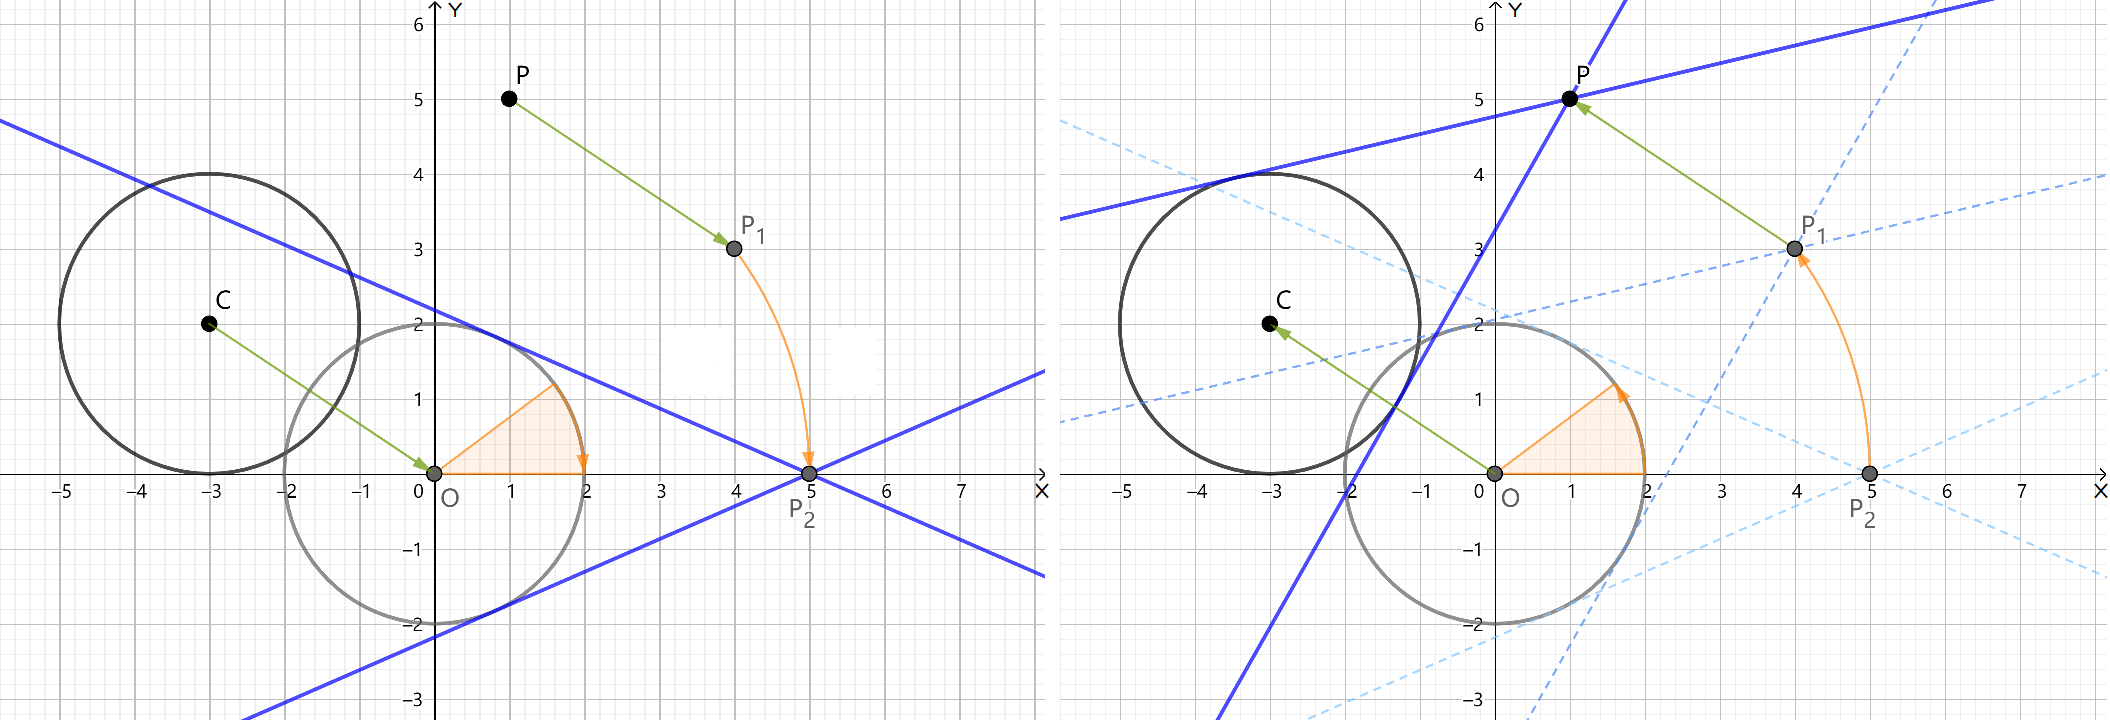
\includegraphics[width=0.9\textwidth]{tu/求切线变换1.png}
    \captionsetup{justification=centering}
    \caption*{\texttt{左:先\textcolor{LimeGreen}{平移}再\textcolor{YellowOrange}{旋转},把圆心移到原点,$P$移到$x$轴上\\ 
                      右:先\textcolor{YellowOrange}{旋转}再\textcolor{LimeGreen}{平移},把$P$点和圆移回,切线随之移动}}
\end{figure}

我们已经知道,如果出发点在$x$轴正半轴上,那么求出一个切点的操作,可以用以下的映射表示:
$$f_1: (x, y) \mapsto \left(\frac{r^2}{x},\,\, \frac{r\sqrt{x^2 - r^2}}{x}\right).$$
考虑圆心在原点,而出发点不在$x$轴正半轴上的情况。这时的图像完成了从$C$到原点的平移,还没有旋转,出发点在$P_1$的位置上。

我们需要把$P_1$点旋转到$x$轴正半轴上的$P_2$点。记这个旋转为$T_\theta$,其中$\theta$是旋转角度。
旋转完成后,我们通过$f_1$映射找到切点,再通过$T$的逆映射$T_\theta^{(-1)}$让$x$轴上的$P_2$点回到$P_1$位置,
而切点经过$T_\theta^{(-1)}$映射的结果,就是$P_1$与圆的切点。
$$T_\theta: P_1 \longrightarrow P_2, \quad T_\theta^{(-1)}: P_2 \longrightarrow P_1.$$

$T_\theta^{(-1)}$是什么呢?我们已经学习过旋转映射。$T_\theta$是以原点为中心,按$\theta$角旋转的映射。它可以表示为:
$$T_\theta: (x,\,\, y) \mapsto (x\cos{\theta} - y\sin{\theta},\,\,y\cos{\theta} + x\sin{\theta}).$$
它的逆映射是以原点为中心,按$-\theta$角旋转的映射:
$$T_{-\theta}: (x,\,\, y) \mapsto (x\cos{\theta} + y\sin{\theta},\,\,y\cos{\theta} - x\sin{\theta}).$$
也就是说,$T_\theta^{(-1)}$就是$T_{-\theta}$。
于是,$P_1$对应的切点可以表示为:$T_{-\theta}\circ f\circ T_\theta(P_1)$,即$P_1$依次经过$T_\theta$、$f_1$、$T_{-\theta}$映射的结果。

记$P_1$的坐标为$(x_P,\,\,y_P)$,则切点坐标为:
\begin{align}
    T_{-\theta}\circ f_1\circ T_\theta(P_1) &= T_{-\theta}\circ f_1(x_P\cos{\theta} - y_P\sin{\theta}) \notag \\
    &= T_{-\theta}\left(\frac{r^2}{x_P\cos{\theta} - y_P\sin{\theta}},\,\, \frac{rs}{x_P\cos{\theta} - y_P\sin{\theta}}\right) \notag \\
    &= \left(\frac{r^2\cos{\theta} + rs\sin{\theta}}{x_P\cos{\theta} - y_P\sin{\theta}},\,\, \frac{-r^2\sin{\theta} + rs\cos{\theta}}{x_P\cos{\theta} - y_P\sin{\theta}}\right) \notag
\end{align}
其中$s = \sqrt{(x_P\cos{\theta} - y_P\sin{\theta})^2 - r^2}$。

这就是$P_1$对应的切点。它的表达式里还包括了$\theta$。$\theta$是把$P_1$旋转到$P_2$的角度。我们知道$P_2$的纵坐标为$0$,
横坐标大于$0$,因此:
$$ y_P \cos{\theta} + x_P\sin{\theta} = 0. $$
解得:
\begin{alignat*}{1}
&   \begin{dcases}
        \cos{\theta} = \frac{x_P}{\sqrt{x_P^2 + y_P^2}} \\
        \sin{\theta} = \frac{-y_P}{\sqrt{x_P^2 + y_P^2}} 
    \end{dcases}
\end{alignat*}
于是$x_P\cos{\theta} - y_P\sin{\theta} = \sqrt{x_P^2 + y_P^2}$。这说明$s^2$就是点到圆的势。
代入切点的表达式,就得到切点坐标为:
\begin{alignat*}{1}
    &   \begin{dcases}
    x_1 = \frac{r(rx_P - sy_P) }{x_P^2+y_P^2} \\
    y_1 = \frac{r(sx_P + ry_P)}{x_P^2+y_P^2}
\end{dcases}
\end{alignat*}
用另一个切点对应的映射:
$$f_2: (x, y) \mapsto \left(\frac{r^2}{x},\,\, -\frac{r\sqrt{x^2 - r^2}}{x}\right),$$
可以算出另一个切点的坐标:
\begin{alignat*}{1}
    &   \begin{dcases}
        x_2 = \frac{r(rx_P + sy_P) }{x_P^2+y_P^2} \\
        y_2 = \frac{r(sx_P - ry_P)}{x_P^2+y_P^2}
    \end{dcases}
\end{alignat*}
我们重新得到了之前的结果。但以上的推导过程能让我们更直观地理解其中发生了什么。

我们看到,这种思考方式可以推广到更一般的情况。考虑平面中图形的关系时,我们可以先将图形变换到适合讨论的位置,
讨论完毕后再变换回去。

以上讨论涉及旋转映射和平移映射。这两种映射有一个共同点,就是它们总把直线变成直线。
只有这样,我们才可能通过出发点和切点讨论变换前后的切线。如果映射不总把直线变成直线,
比如切线经过映射变成了曲线,我们就没法用出发点和切点确定切线了。

我们已经定义过,把平面的点(向量)映射到平面的点的映射,叫做平面的\textbf{点映射}。
点映射大致可以用来描述平面形的变换。

如果平面的点映射满足以下性质:
\begin{enumerate}
    \item 与平移操作可以交换顺序。
    \item 与过原点的放缩操作可以交换顺序。
\end{enumerate}
就比较好研究。我们把这类映射称为\textbf{直映射}或\textbf{直变换}。具体来说,直变换$f$满足:
\begin{enumerate}
    \item $\forall \,\,\mathbf{u}, \,\,\mathbf{v}$,$f(\mathbf{u} + \mathbf{v}) = f(\mathbf{u}) + f(\mathbf{v})$
    \item $\forall \,\,k, \,\, \mathbf{u}$,$f(k\cdot \mathbf{u}) = k \cdot f(\mathbf{u})$
\end{enumerate}
直变换有以下的基本性质:
\begin{tm}
    直变换总把原点映射到原点。
\end{tm}
\begin{proof}
    $$f(\mathbf{0}) = f(0\cdot \mathbf{0}) = 0 \cdot f(\mathbf{0}) = \mathbf{0}.$$
\end{proof}
\begin{tm}
    直变换总把直线映射为直线或点。
\end{tm}
\begin{proof}
    设有直变换$f$,直线$l: \mathbb{R}\mathbf{a} + \mathbf{b}$。
    给定直线中任一点$t\mathbf{a} + \mathbf{b}$,它经过映射$f$变为:$f(t\mathbf{a} + \mathbf{b})$。
    按照$f$的性质:
    $$ f(t\mathbf{a} + \mathbf{b}) = tf(\mathbf{a}) + f(\mathbf{b}).$$
    因此总在集合$\{tf(\mathbf{a}) + f(\mathbf{b})\,|\, t\in\mathbb{R}\}$中。
    我们把这个集合记作$\mathbb{R}f(\mathbf{a}) + f(\mathbf{b})$。
    反之,集合$\mathbb{R}f(\mathbf{a}) + f(\mathbf{b})$中每一点显然也是$l$中某点经过$f$映射的结果。
    也就是说,$l$经过映射得到的集合就是$\mathbb{R}f(\mathbf{a}) + f(\mathbf{b})$:
    $$ f(\mathbb{R}\mathbf{a} + \mathbf{b}) = \mathbb{R}f(\mathbf{a}) + f(\mathbf{b}).$$
    如果$f(\mathbf{a})$是非零向量,那么$\mathbb{R}f(\mathbf{a}) + f(\mathbf{b})$是一条直线。
    如果$f(\mathbf{a})$是零向量,那么$\mathbb{R}f(\mathbf{a}) + f(\mathbf{b}) = \{f(\mathbf{b})\}$是一个点。

    综上,$f$总把直线映射为直线或点。
\end{proof}

显然,只要$f$把任一个非零向量映射为零向量,它就会把相应方向的直线映射为点。
因此,直变换$f$总把直线映射为直线,当且仅当它是满射。

进一步还可以发现,
\begin{tm}
    直变换如果是满射,那么总把数轴变换为数轴。
\end{tm}
因此,直变换也称为\textbf{轴映射}或\textbf{轴变换}。
\begin{proof}
    首先直变换总把原点映射到原点。给定直变换$f$。如果$f$是满射,那么它总将直线映射为直线。
    设有数轴$l$,它是一条过原点的直线$l: \mathbb{R}\mathbf{a}$,正方向和单位长度由向量$\mathbf{a}$表示。
    $f$将它映射为直线$\mathbb{R}f(\mathbf{a})$。

    考虑$l$上任两点$s\mathbf{a}$、$t\mathbf{a}$,它经过$f$映射为
    $$ f(s\mathbf{a}) = sf(\mathbf{a}),\qquad f(t\mathbf{a}) = tf(\mathbf{a}).$$
    可以看出,数轴上的点经过$f$映射后,到原点距离之比不变。也就是说,数轴上的“刻度”,经过映射,可以作为新数轴的刻度。
    新数轴的正方向和单位长度由向量$f(\mathbf{a})$表示。
\end{proof}

哪些点映射是直变换呢?

以原点为中心的旋转映射就是一种直变换。
除了旋转映射,以过原点的直线为对称轴的轴对称变换和以原点为中心的位似映射也是直变换,
而平移映射则不是直变换。不过,由于平移映射也把直线映射为直线,我们可以考虑直变换和平移映射的复合。

\begin{df}
    如果一个映射能表示为平移映射与直变换的复合,
    就说它是\textbf{维直变换}。具体来说,维直变换$f$总可以写成:
    $$ f: \,\, \vv{x} \mapsto a(\vv{x}) + \vv{b} $$
    其中$a$是直变换,$\vv{b}$是平移的向量。
\end{df}
不难发现,维直变换也总把直线映射为直线或点。维直变换是满射,当且仅当它总把直线映射为直线。

怎样的映射是直变换呢?我们从平面的基底出发进行思考。给定平面基底$B = (\mathbf{e}_1, \mathbf{e}_2)$,
平面中任何向量$\mathbf{u}$都可以表示为基底的直组合:
$$ \mathbf{u} = u_1 \mathbf{e}_1 + u_2 \mathbf{e}_2.$$
其中$u_1, u_2$是向量$\mathbf{u}$关于该基底的坐标。考虑$\mathbf{u}$经过直变换$f$的结果$f(\mathbf{u})$。
按照$f$的性质:
$$ f(\mathbf{u}) = f(u_1 \mathbf{e}_1 + u_2 \mathbf{e}_2) = u_1 f(\mathbf{e}_1) + u_2 f(\mathbf{e}_2).$$
其中$f(\mathbf{e}_1)$、$f(\mathbf{e}_2)$是基向量经过$f$映射得到的向量。
因此,只要知道了直变换在某个基底上的效果,就能知道直变换对任意向量的效果。
\textbf{直变换的性质由它在某个基底上的映射结果确定}。

\section{直变换的矩阵表示}

具体来说,怎样描述直变换的性质呢?
从上面的结论继续思考。$f(\mathbf{e}_1)$、$f(\mathbf{e}_2)$这两个向量也可以表示成$\mathbf{e}_1, \mathbf{e}_2$的直组合:
\begin{align}
    f(\mathbf{e}_1) &= a_{11} \mathbf{e}_1 + a_{21} \mathbf{e}_2 \notag \\
    f(\mathbf{e}_2) &= a_{12} \mathbf{e}_1 + a_{22} \mathbf{e}_2 \notag
\end{align}
也就是说,
$$ f(\mathbf{u}) = u_1 f(\mathbf{e}_1) + u_2 f(\mathbf{e}_2) = (u_1a_{11} + u_2a_{12}) \mathbf{e}_1 + (u_1a_{21} + u_2a_{22}) \mathbf{e}_2.$$

比如,前面提到的旋转映射$T$就可以写成这样的形式。设有旋转映射$T$将坐标为$(x,\,\, y)$的点变换到$(x\cos{\alpha} - y\sin{\alpha},\,\,y\cos{\alpha} + x\sin{\alpha})$。
那么,基底向量$\mathbf{e}_x, \mathbf{e}_y$分别被变换到:
\begin{align}
    T(\mathbf{e}_x) &= \cos{\alpha}\,\mathbf{e}_x + \sin{\alpha}\,\mathbf{e}_y \notag \\
    T(\mathbf{e}_y) &= -\sin{\alpha}\,\mathbf{e}_x + \cos{\alpha}\,\mathbf{e}_y \notag 
\end{align}
即:
$$
\begin{array}{rlrl}
    a_{11} &= \cos{\alpha}, \quad & a_{21} &= \sin{\alpha} \\
    a_{12} &= -\sin{\alpha}, \quad & a_{22} &= \cos{\alpha} \\
\end{array}
$$

我们把向量用另一种方式表记,比如坐标为$(x, \,\,y)$的向量记为:
$$ \begin{bmatrix}
    x\\ y
\end{bmatrix}$$
于是,向量$\mathbf{u}$经过直变换$f$得到新向量可以写成:
$$ f\left(\begin{bmatrix}
    u_1\\ u_2
\end{bmatrix}\right) = u_1\begin{bmatrix}
    a_{11}\\ a_{21}
\end{bmatrix} + u_2 \begin{bmatrix}
    a_{12}\\ a_{22}
\end{bmatrix} = \begin{bmatrix}
    u_1a_{11} + u_2a_{12}\\ u_1a_{21} + u_2a_{22} 
\end{bmatrix}.$$
可以看到,给定基底$B$之后,直变换$f$可以用系数$a_{11}$、$a_{12}$、$a_{21}$、$a_{22}$来表示,
因此,为了方便,我们可以把直变换$f$记为:
$$
[\,f\,]_B = 
\begin{bmatrix}
    a_{11} & a_{12} \\ a_{21} & a_{22}
\end{bmatrix}
$$
即把基向量经过$f$得到的新向量左右合并起来。
我们把这样的阵列称为\textbf{矩阵},这种表示直变换的方法称为直变换在给定基底$B$上的\textbf{矩阵表示}。

一般来说,矩阵就是把数写成行列的形式。
\begin{df}{\textbf{矩阵}}
    \mbox{}\\
    设$m,n$为正整数。把$m \times n$个元素写成$m$行,每行$n$个,对齐为$n$列。
    就说这是一个$m$行$n$列的\textbf{矩阵},也叫做$m \times n$的矩阵。\\
    矩阵自上起第$i$行、左起第$j$列的元素叫做矩阵第$i$行第$j$列的元素,一般用下标$ij$或$i,j$指示。
\end{df}

$f$的矩阵有两行两列,可以说它是一个$2\times 2$的矩阵。

广泛意义上说,把向量表示为
$$ \begin{bmatrix}
    x\\ y
\end{bmatrix},$$
也可以看成一个$2\times 1$的矩阵(两行一列)。因此我们可以用矩阵记录向量经历直变换的过程:
$$ \begin{bmatrix}
    a_{11} & a_{12} \\ a_{21} & a_{22}
\end{bmatrix}\begin{bmatrix}
    u_1\\ u_2
\end{bmatrix} = u_1\begin{bmatrix}
    a_{11}\\ a_{21}
\end{bmatrix} + u_2 \begin{bmatrix}
    a_{12}\\ a_{22}
\end{bmatrix} = \begin{bmatrix}
    u_1a_{11} + u_2a_{12}\\ u_1a_{21} + u_2a_{22} 
\end{bmatrix}.$$

反过来,给定基底$B = (\mathbf{e}_1, \,\,\mathbf{e}_2)$之后,任意给定四个数$a_{11}$、$a_{12}$、$a_{21}$、$a_{22}$,都可以构造映射$f$:
$$ \forall \,\, u_1, u_2 \in \mathbb{R}, \quad  f(u_1\mathbf{e}_1 + u_2\mathbf{e}_2) = (u_1a_{11} + u_2a_{12}) \mathbf{e}_1 + (u_1a_{21} + u_2a_{22}) \mathbf{e}_2.$$
这样定义的映射是直变换。

\begin{proof}
    首先,对任意$\mathbf{u} = (u_1,\,\, u_2)$、$\mathbf{v} = (v_1,\,\,v_2)$,
    \begin{align}
        f (\mathbf{u} + \mathbf{v}) &= f \big((u_1 + v_1,\,\, u_2 + v_2)\big) \notag \\
        &= \Big((u_1 + v_1)a_{11} + (u_2 + v_2)a_{12},\,\,(u_1 + v_1)a_{21} + (u_2 + v_2)a_{22}\Big)\notag \\
        &= (u_1a_{11} + u_2a_{12},\,\,u_1a_{21} + u_2a_{22}) + (v_1a_{11} + v_2a_{12},\,\,v_1a_{21} + v_2a_{22})\notag \\
        &= f (\mathbf{u}) + f (\mathbf{v}). \notag
    \end{align}
    其次,对任意向量$\mathbf{u}$和任意实数$k$,
    \begin{align}
        f (k\mathbf{u}) &= f \big((ku_1,\,\, ku_2)\big) \notag \\
        &= (ku_1a_{11} + ku_2a_{12},\,\,ku_1a_{21} + ku_2a_{22})\notag \\
        &= k(u_1a_{11} + u_2a_{12},\,\,u_1a_{21} + u_1a_{22})\notag \\
        &= kf (\mathbf{u}). \notag
    \end{align}  
    综上所述,$f$是直变换。
\end{proof}

也就是说,给定$2\times 2$的矩阵,那么它对应一个直变换。

这说明,固定平面的基底时,每个直变换恰好对应一个$2\times 2$矩阵。

\begin{sk}
    \mbox{} \\
    \indent 1. 映射$f$把平面上的点映射到平面上的点。如果$f$总把直线变成直线,$f$是否总能表示成直变换和平移映射的复合?\\
    \indent 2. 直变换在不同基底上的矩阵是否总是不一样?对于不同的基底,同一个矩阵是否总对应不同的直变换?
\end{sk}

\begin{xt}
    \mbox{} \\
    \indent 1. 在求切线方程的例子中,补全用另一个切点对应的映射$f_2$求出切 \\
    \indent 点的过程。\\
    \indent 2. 写出以下直变换的矩阵;\\
    \indent 2.1. $f: \,\, (x,\,\, y) \mapsto (x + 2y,\,\, y - 3x)$ \\
    \indent 2.2. $f: \,\, f(\mathbf{e}_1) = -\mathbf{e}_1 - \mathbf{e}_2,\,\,\, f(\mathbf{e}_2) = \mathbf{e}_1 - \mathbf{e}_2$ \\
    \indent 2.3, $f: \,\, f(\mathbf{e}_1 + \mathbf{e}_2) = \mathbf{e}_1 - \mathbf{e}_2,\,\,\, f(\mathbf{e}_2 - \mathbf{e}_1) = \mathbf{e}_1 + \mathbf{e}_2$ \\
    \indent 3. 给定基底$B$,写出以下矩阵对应的点映射$f$,以及向量$\mathbf{v}$经过该映射的结果。\\
    \indent 3.1. $$
                [\,f\,]_B = 
                \begin{bmatrix}
                    5 & -1 \\ 0 & 2
                \end{bmatrix},\quad \mathbf{v} = \begin{bmatrix}
                    1\\ 3
                \end{bmatrix}
                $$
    \indent 3.2. $$
                [\,f\,]_B = 
                \begin{bmatrix}
                    -2 & 4 \\ -3 & 1
                \end{bmatrix},\quad \mathbf{v} = \begin{bmatrix}
                    -7\\ 1
                \end{bmatrix}
                $$
    \indent 3.3. $$
                [\,f\,]_B = 
                \begin{bmatrix}
                    0 & 3 \\ 3 & 2
                \end{bmatrix},\quad \mathbf{v} = \begin{bmatrix}
                    -1\\ 1
                \end{bmatrix}
                $$
\end{xt}

\section{各种直变换}
定义了直变换之后,我们来看一些具体的例子。
首先是把所有向量映射到零向量的\textbf{零映射},和把所有向量映射到自身的\textbf{恒等映射}。
不难验证,这两种映射都是直变换。

以原点为中心的\textbf{位似映射}也是直变换:
$$ F_k : \mathbf{u} \mapsto k\mathbf{u}.$$
它的矩阵是:
$$
\begin{bmatrix}
    k & 0 \\ 0 & k
\end{bmatrix}
$$

上一节的例子已经给出了以原点为中心的\textbf{旋转映射}的矩阵。
以原点为中心,按$\theta$角(逆时针)旋转的映射可以表示为:
$$T_{\theta}: (x,\,\, y) \mapsto (x\cos{\theta} - y\sin{\theta},\,\,y\cos{\theta} + x\sin{\theta}).$$
也就是说,它可以用以下的矩阵表示:
$$
\begin{bmatrix}
    \cos{\theta} & -\sin{\theta} \\ \sin{\theta} & \cos{\theta}
\end{bmatrix}
$$
它把直角坐标系的基向量$\mathbf{e}_1 = (1,\,\,0)$和$\mathbf{e}_2 = (0,\,\,1)$分别映射到
$(\cos{\theta},\,\,\sin{\theta})$和$(-\sin{\theta},\,\,\cos{\theta})$,也就是矩阵的两列对应的向量。

根据上一节的结论,$T_{\theta}$是直变换。 

再来看\textbf{投影映射}。
给定不共轴的向量$\mathbf{a}$、$\mathbf{b}$,沿$\mathbf{b}$到$\mathbf{a}$的投影映射为:
$$ \mathrm{Ty}_{\mathbf{a}, \mathbf{b}} : \,\,\, \mathbf{u} \mapsto u_a \mathbf{a} $$
其中$u_a$是向量$\mathbf{u}$按$\mathbf{a}$、$\mathbf{b}$分解时,分量$\mathbf{a}$的系数。

比如:
$$ P: (x,\,\, y) \mapsto (x,\,\,0)$$
它将向量$(x,\,\, y)$的纵坐标变成$0$。

$\mathrm{Ty}_{(\mathbf{a},\mathbf{b})}$把$\mathbf{a}$映射到自身,而把$\mathbf{b}$映射到零向量。
于是,以$\mathbf{a}$、$\mathbf{b}$为基底时,我们可以把它写成矩阵的形式:
$$
\begin{bmatrix}
    1 & 0 \\ 0 & 0
\end{bmatrix}
$$

矩阵的两列分别表示$\mathbf{a}$、$\mathbf{b}$投影后的结果。

根据上一节的结论,投影变换也是直变换。

最后来看\textbf{反射映射}。
给定向量$\mathbf{a}$、$\mathbf{b}$,沿$\mathbf{b}$到$\mathbf{a}$的反射映射为:
$$ \mathrm{Fs}_{\mathbf{a}} : \,\,\, \mathbf{u} \mapsto u_a \mathbf{a} - u_b \mathbf{b} $$
其中$u_a, u_b$是向量$\mathbf{u}$按$\mathbf{a}$、$\mathbf{b}$分解的系数。

比如:
$$ S: (x,\,\,y) \mapsto (x,\,\, -y) $$
就是以$x$轴为对称轴的反射映射。

$\mathrm{Fs}_{(\mathbf{a},\mathbf{b})}$把$\mathbf{a}$映射到自身,而把$\mathbf{b}$映射到$-\mathbf{b}$。
于是,以$\mathbf{a}$、$\mathbf{b}$为基底时,我们可以把它写成矩阵的形式
$$
\begin{bmatrix}
    1 & 0 \\ 0 & -1
\end{bmatrix}
$$

因此,反射映射也是直变换。

以上几种点映射,除了旋转映射,都可以看作以下这种映射的特例:
$$ H_{(\mathbf{a},\mathbf{b})}^{s, t}: \mathbf{u} \mapsto su_a\mathbf{a} + tu_b\mathbf{b}.$$
其中$\mathbf{a}$、$\mathbf{b}$是不共轴的向量,$(u_a,\,\,u_b)$是$\mathbf{u}$在$\mathbf{a}$、$\mathbf{b}$构成的坐标系中的坐标。
而$s,t$分别表示向量经过映射之后,在$\mathbf{a}$、$\mathbf{b}$方向缩放的比例。

不难验证,随着$s,t$取不同的值,我们就得到不同类型的点映射:
\begin{enumerate}
    \item 令$s = t = 0$,我们得到零映射;
    \item 令$s = t = 1$,我们得到恒等映射;
    \item 令$s = t = k$,我们得到相似比为$k$的位似映射;
    \item 令$s = 1$、$t = 0$,我们得到投影映射;
    \item 令$s = 1$、$t = -1$,我们得到反射映射。
\end{enumerate}

$H_{(\mathbf{a},\mathbf{b})}^{s, t}$把$\mathbf{a}$映射到$s\mathbf{a}$,而把$\mathbf{b}$映射到$t\mathbf{b}$。
于是,以$\mathbf{a}$、$\mathbf{b}$为基底时,我们可以写出它的矩阵:
$$
\begin{bmatrix}
    s & 0 \\ 0 & t
\end{bmatrix}
$$
可以看到,$s,t$在矩阵从左上到右下的对角线上。矩阵除了对角线以外的地方都是$0$。
我们把这样的矩阵称为\textbf{对角矩阵},把$H_{(\mathbf{a},\mathbf{b})}^{s, t}$称为
(关于$\mathbf{a}$、$\mathbf{b}$构成的基底的)\textbf{对角映射},
把$s,t$称为它的\textbf{变化系数}。

按照上一节的结论,对角映射总是直变换。

零映射、恒等映射、位似映射、投影映射、反射映射都是对角映射。

除了旋转映射和对角映射,还有一类基本的直变换。给定基底$\mathbf{e}_x, \mathbf{e}_y$和实数$t$,考虑矩阵为:
$$
\begin{bmatrix}
    1 & t \\ 0 & 1
\end{bmatrix}
$$
的变换$J_t$。它把基向量$\mathbf{e}_x$映射为$\mathbf{e}_x + t\mathbf{e}_y$,
把基向量$\mathbf{e}_y$映射到自身。给定标准单位正方形,$J_t$把它变为同底等高的平行四边形。

% 错切变换:正方形变为同底等高的平行四边形
\begin{figure}[h]
    \vspace{4pt}
    \centering
    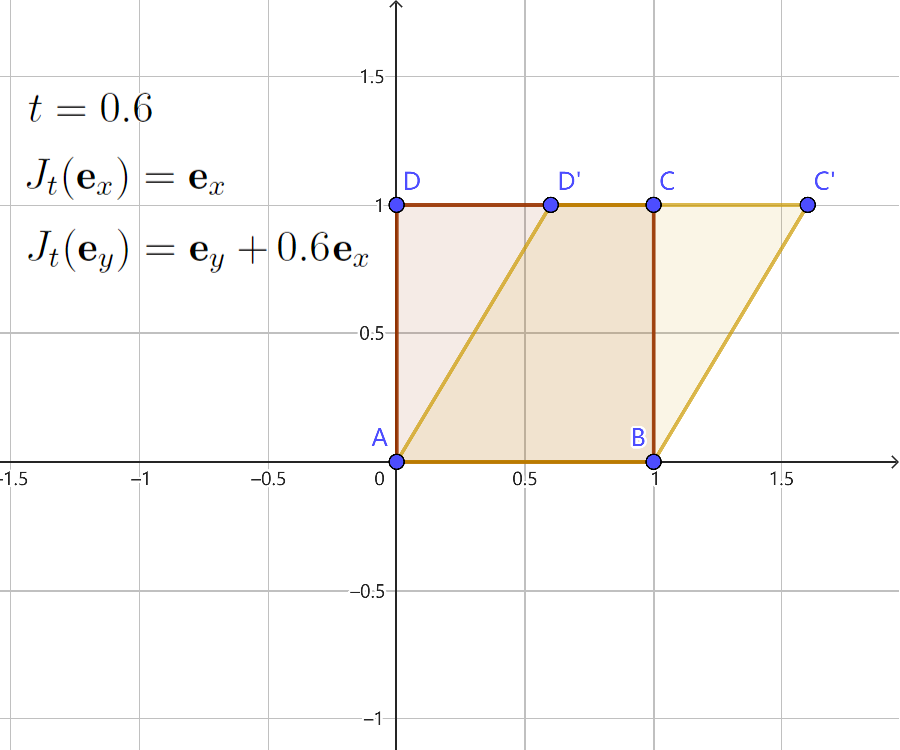
\includegraphics[width=0.6\textwidth]{tu/剪变换1.png}
    \captionsetup{justification=centering}
    \caption*{\texttt{剪变换}$J_t$\texttt{把\textcolor[RGB]{162,69,22}{标准单位正方形}变换为\textcolor[RGB]{218,183,74}{平行四边形}}}

\end{figure}

现实的工程问题中常常会遇到这个变换。
它可以用来描述物体的不同位置受到两个大小相同、方向相反的力,
而产生形变的过程,比如用剪刀裁剪物体,尚未剪断时物体形状的变化。
因此,我们把这种变换叫做\textbf{剪映射}或\textbf{错切映射}。

% 剪刀示意图

\begin{sk}
    \mbox{} \\
    \indent 1. 零映射、恒等映射、位似映射、旋转映射、投影映射、反射映射、剪映射,哪些是单射,哪些是满射,哪些是双射?\\
    \indent 2. 一个点映射是否可能既是旋转映射,又是反射映射?既是旋转映射,又是位似映射?反射映射,又是位似映射?\\
    \indent 3. 零映射、恒等映射、位似映射、旋转映射、投影映射、反射映射、剪映射是否有逆映射?如果有的话,是什么样的映射?
\end{sk}

\begin{xt}
    \mbox{} \\
    \indent 1. 写出以原点为中心,相似比为$2.5$的位似映射及其矩阵。求$(2,\,\,-1)$经过映射的结果。\\
    \indent 2. 写出以原点为中心,顺时针旋转$90^\circ$的旋转映射及其矩阵。求$(2,\,\,-1)$经过映射的结果。\\
    \indent 3. 给定直角坐标系,写出沿$(1,\,\,3)$到$(2,\,\,0)$的投影映射。求$(2,\,\,-1)$经过映射的结果。\\
    \indent 4. 给定直角坐标系,写出关于$(-1,\,\,-4)$的反射映射。求$(2,\,\,-1)$经过映射的结果。\\
    \indent 5. 给定直角坐标系。关于直角坐标系基底的对角映射$f$把向量$(3,\,\,1)$映射到$(-4,\,\,2)$。
               求$f$的变化系数,写出它的矩阵。求$(2,\,\,-1)$经过映射的结果。\\
    \indent 6. 给定平面基底,直变换$f$可以写成矩阵的形式:
                $$
                \begin{bmatrix}
                    1 & 0 \\ t & 1
                \end{bmatrix}
                $$
                其中$t$是实数。那么,$f$是怎样的映射?
\end{xt}

\section{基底变换}

让我们再换一个角度看一开始的求切线问题。变换是相对的。我们把图形变换位置,相对的是平面的坐标系。
那么,我们能否把这些变换看成坐标系的变换呢?

考虑平面中图形的关系时,我们可以根据图形特点,选择合适的坐标系,在这个坐标系中讨论,讨论完毕后再变换到另一个坐标系,展示讨论的结果。

从这个角度来看,之前的讨论可以看作是对平面的坐标系进行变换。
我们把坐标系转移到圆心处,让$x$轴正方向对准出发点,在这个坐标系下求出切点,再转回原来的坐标系。

让我们用向量的语言来具体说明。仍然从圆心平移到原点后的情况出发,设出发点在这个坐标系里的坐标是$(x_P,\,\,y_P)$。
坐标系对应一组基底向量:$\mathbf{e}_x, \mathbf{e}_y$。出发点可以表示为:
$$ x_P\mathbf{e}_x + y_P\mathbf{e}_y. $$
我们希望找出一组新的坐标系,对应另一组基底向量:$\mathbf{e}_x', \mathbf{e}_y'$,使得出发点在新坐标系的纵坐标是$0$,而横坐标大于$0$。

按照前面的发现,我们作旋转映射来找出这组基底。
设有旋转映射$T$将坐标为$(x,\,\, y)$的点变换到$(x\cos{\alpha} - y\sin{\alpha},\,\,y\cos{\alpha} + x\sin{\alpha})$。
因此,基底向量$\mathbf{e}_x, \mathbf{e}_y$分别被变换到:
\begin{align}
    \mathbf{e}_x' = T(\mathbf{e}_x) &= \cos{\alpha}\,\mathbf{e}_x + \sin{\alpha}\,\mathbf{e}_y \notag \\
    \mathbf{e}_y' = T(\mathbf{e}_y) &= -\sin{\alpha}\,\mathbf{e}_x + \cos{\alpha}\,\mathbf{e}_y \notag 
\end{align}
我们希望出发点在新坐标系里纵坐标是$0$,而横坐标大于$0$。设出发点在新坐标系的坐标是$(x_P', \,\, y_P')$,
那么我们希望$x_P' > 0$,$y_P' = 0$。即:
$$ x_P\mathbf{e}_x + y_P\mathbf{e}_y = x_P' \mathbf{e}_x' + 0 \cdot \mathbf{e}_y' = x_P' (\cos{\alpha}\,\mathbf{e}_x + \sin{\alpha}\,\mathbf{e}_y). $$
于是,根据平面基本定理,两个基向量的系数分别相等:
\begin{alignat*}{1}
&   \begin{dcases}
        x_P = x_P' \cos{\alpha} \\
        y_P = x_P' \sin{\alpha} 
    \end{dcases}
\end{alignat*}
于是:
$$ x_P'^2 = x_P'^2 (\cos^2{\alpha} + \sin^2{\alpha}) = x_P^2 + y_P^2. $$
解得$x_P' = \sqrt{x_P^2 + y_P^2}$,因此:
\begin{alignat*}{1}
&   \begin{dcases}
        \cos{\alpha} = \frac{x_P}{\sqrt{x_P^2 + y_P^2}} \\
        \sin{\alpha} = \frac{y_P}{\sqrt{x_P^2 + y_P^2}} 
    \end{dcases}
\end{alignat*}

不难看出,这里的旋转角$\alpha$是前面旋转映射的旋转角$\theta$的相反数:
$$ \alpha = -\theta.$$
这并不难理解。保持平面不变,把平面中的图形按$\theta$旋转,和保持平面中的图形不变,
把整个平面按反方向旋转同样的角度,效果是一样的。旋转映射是直变换,保持原点不变、直线仍是直线、
长度比例不变。直观上说,平面经过旋转,仍然是平的,直线仍然是直的,坐标轴仍然是坐标轴。

除了旋转映射,可以验证,以原点为中心的位似映射和以过原点直线为轴的轴对称映射也满足这些性质。
实际上,我们可以把这一类映射归结为基底的变换。

一般来说,把平面的一组基底变为另一组基底的直变换,叫做\textbf{基底变换},简称\textbf{基变换}或\textbf{基变更}。
直观上看,基变换就是把两条数轴变换成另外两条数轴。

怎样用基变换描述坐标的变换呢?

原有的基底$B$记为$\mathbf{e}_1, \mathbf{e}_2$。
某个基底变换$h$将$B$变为新基底$B'$。具体来说,$h$把$\mathbf{e}_1$变为$\mathbf{e}_1' = a_{11}\mathbf{e}_1 + a_{21}\mathbf{e}_2$,
把$\mathbf{e}_2$变为$\mathbf{e}_2' = a_{12}\mathbf{e}_1 + a_{22}\mathbf{e}_2$。
那么,$h$在基底$B$上的矩阵是:
$$
\left[h\right]_{B} = 
\begin{bmatrix}
    a_{11} & a_{12} \\ a_{21} & a_{22}
\end{bmatrix}
$$

设某个点$P$在原基底$B$上的坐标为$(s,\,\, t)$,那么$P$点在新基底的坐标是多少呢?

设$P$在新基底的坐标为$(x,\,\, y)$,那么:
$$ s\mathbf{e}_1 + t\mathbf{e}_2 = x\mathbf{e}_1' + y\mathbf{e}_2'.$$
将$\mathbf{e}_1'$、$\mathbf{e}_2'$用$\mathbf{e}_1$、$\mathbf{e}_2$的直组合表示,就得到:
\begin{align}
    s\mathbf{e}_1 + t\mathbf{e}_2 &= x(a_{11}\mathbf{e}_1 + a_{21}\mathbf{e}_2) + y(a_{12}\mathbf{e}_1 + a_{22}\mathbf{e}_2) \notag \\
    &= (a_{11}x + a_{12}y)\mathbf{e}_1 + (a_{21}x + a_{22}y)\mathbf{e}_2 \notag
\end{align}
也就是说,$x, y$是以下二元一次方程组的解:
\begin{alignat*}{1}
    &   \begin{dcases}
            a_{11}x + a_{12}y = s \\
            a_{21}x + a_{22}y = t
        \end{dcases}
\end{alignat*}

\begin{figure}[h]
    \vspace{4pt}
    \centering
    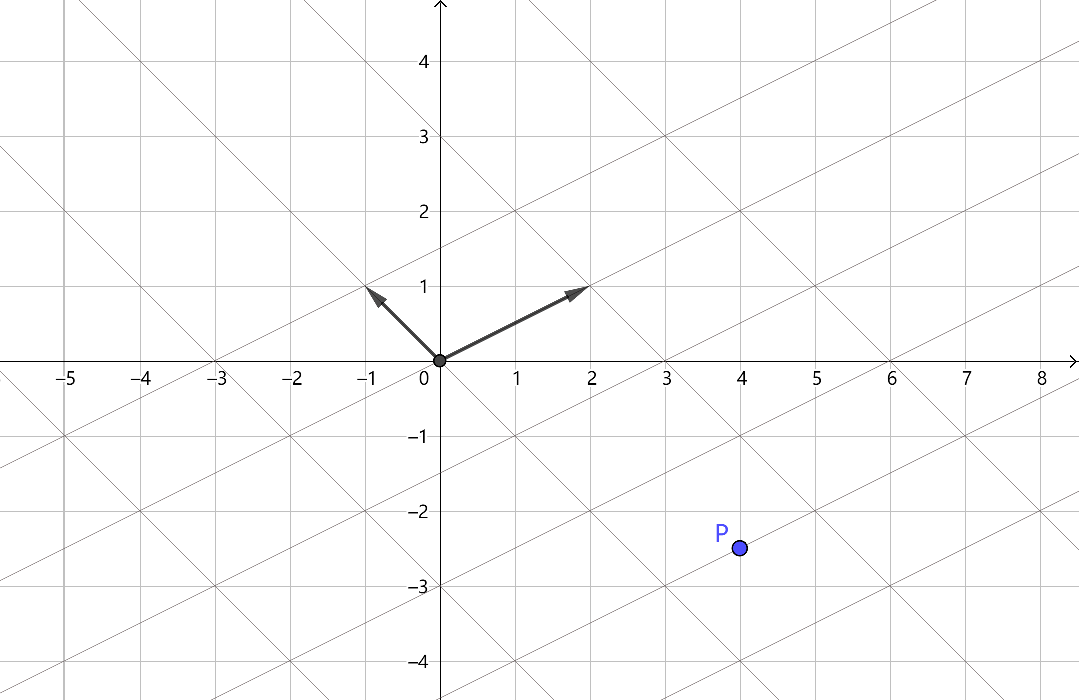
\includegraphics[width=0.9\textwidth]{tu/基变换1.png}
    \captionsetup{justification=centering}
\end{figure}

来看一个具体的例子。设基变换$h$在原基底上的矩阵为
$$
\left[h\right]_{B} = 
\begin{bmatrix}
    2 & -1 \\ 1 & 1
\end{bmatrix}
$$
点$P$在原基底上的坐标为$(4,\,\, -2.5)$,新基底上的坐标为$(x_P,\,\, y_P)$,则:
\begin{alignat*}{1}
    &   \begin{dcases}
            2x_P  - y_P = 4 \\
            x_P + y_P = -2.5
        \end{dcases}
\end{alignat*}
解得:
\begin{alignat*}{1}
    &   \begin{dcases}
            x_P = 0.5 \\
            y_P = -3
        \end{dcases}
\end{alignat*}
$P$在新基底上的坐标为$(0.5, \,\, -3)$。我们可以从上图中直接观察到这个结论。

\begin{xt}
    \mbox{} \\
    \indent 1. 证明:基底变换总是满射。直变换是基底变换,当且仅当它是满射。\\
    \indent 2. 设基变换的矩阵为:
    $$
    \begin{bmatrix}
        -2 & 1 \\ 1 & 2
    \end{bmatrix}
    $$
    \indent 某点在原基底的坐标为$(4,\,\,3)$,求它在新基底的坐标。\\
    \indent 3. 设基变换的矩阵为:
    $$
    \begin{bmatrix}
        -1 & 2 \\ 1 & -1
    \end{bmatrix}
    $$
    \indent 某点在新基底的坐标为$(-3,\,\,1)$,求它在原基底的坐标。\\
    \indent 4. 设有平面上的直变换$f$。它在基底$B$上的矩阵为:
    $$
    \left[f\right]_{B} = 
    \begin{bmatrix}
        2 & 1 \\ 0 & -1
    \end{bmatrix}
    $$
    \indent 基变换$h$将基底$B$变为新基底$B'$。它在$B$上的矩阵为:
    $$
    \left[h\right]_{B} = 
    \begin{bmatrix}
        -1 & 1 \\ 1 & 1
    \end{bmatrix}
    $$
    \indent 4.1. 求原基底上的点$(1,\,\,0)$和$(0,\,\,1)$经过$f$变换后,在新基底的坐标。\\
    \indent 4.2. 求新基底上的点$(a,\,\,b)$经过$f$变换后,在新基底的坐标。\\
    \indent 4.3. 写出$f$在新基底上的矩阵$[f]_{B'}$。\\
    \indent 4.4. 能否用$[f]_{B}$和$[h]_{B}$来表示$[f]_{B'}$?
\end{xt}

\chapter{空间中的形状}

我们已经通过公理体系研究过平面中的简单形状,将基本的平面形和函数的图像联系起来,并且引入了向量的概念。
现在,我们进一步研究立体空间中的形状。人类生活在立体空间中,因此,研究空间中形体的性质,对我们认识世界、
改造世界有直接帮助。为了更好地理解以下的内容,我们建议你准备一把刻度尺和足够的白纸。
至于如何在纸面上画出立体形状,可以参考\textbf{附录A}。

\section{点、直线、平面}

和平面形一样,立体空间中的形也是从现实中种种事物的形状总结提炼而来。平面是人类最早总结出的概念之一。
我们已经研究过平面中的形状,因此,研究立体空间时,我们把平面作为地位和点、直线相同的基本概念。

研究平面形状时,我们首先引进了公理体系。如今我们将平面公理体系扩展为立体空间的公理体系。
为此,我们要通过公设和公理定义\textbf{平面}以及它和点、直线的关系。

我们定义面为点的集合,也是线运动的结果。平面是最基本的面,一般用小写希腊字母$\alpha,\beta,\gamma$等表示。
\begin{po}{\textbf{平面公理}}\label{po:0}
    过不共轴的三点,有且仅有一个平面。
\end{po}

我们也说三角形(或圆)确定一个平面。不共轴的三点$A$、$B$、$C$确定的平面,可以记作平面$ABC$。

如何确定平面是“平”的呢?生活和生产中,我们一般用直线来确定一个面是不是平的。
比如,木工常常用角尺的直角边放在刨好的木板上。如果直角边总能与板面紧密贴合,就说明木板已刨平了。
水泥工用直的刮子将刚铺水泥的地面刮平。我们把人们总结出的经验作为判断平面的方法,用公理的形式确定下来。
\begin{po}{\textbf{平直公理}}\label{po:1}
    过平面上不重合两点的直线,在平面中。
\end{po}
平直公理说明,直线要么与平面没有公共点,要么只交于一点,要么全部在平面里。
直线与平面没有公共点,则称直线与平面平行,也用$\parallel$表记;直线与平面恰有一公共点,
则称直线与平面相交;直线与平面有两个或以上公共点,则称直线在平面中或平面经过直线。
用集合的语言来说,直线$l$在平面$\gamma$中,就说明$l$是$\gamma$的子集。

% 我们知道,直线把平面分为两部分,称为直线的两侧。空间中,我们把每侧称为半平面。
% 直线及其一侧的半平面构成一个展面。而每个平面又把空间分为两部分,称为平面的两方。根据实际需要,我们可以称一点在平面的上方或下方、前方或后方、左方或右方,等等。

从平面公理和平直公理,容易得到另两种定义平面的方法:
\begin{tm}\label{tm:1-0-0}
    过一条直线与该直线外一点,有且仅有一个平面。
\end{tm}
\begin{proof}
    设直线为$l$,$P$为$l$外一点。取$l$上不同的两点,和$P$构成不共轴的三点。这三点确定一个平面。
    根据平直公理,$l$在该平面中。
\end{proof}
\begin{tm}\label{tm:1-0-1}
    过两条相交的直线,有且仅有一个平面。
\end{tm}
\begin{proof}
    设有直线$l,m$。如果$l,m$相交,设交点为$P$,在$l,m$上各取不同于$P$的一点:$Q,R$,则$P,Q,R$不共轴,
    于是确定一个平面$PQR$,根据平直公理,$l,m$都在$PQR$中。
\end{proof}

设直线$l$与平面$\gamma$平行,没有公共点,那么它与$\gamma$中任何直线没有公共点。
比如,给定$\gamma$中一点$A$,$\gamma$中经过$A$的任何直线,都与$l$没有公共点。

平面中,两直线没有公共点,就说它们相互平行。空间中,两直线除了重合、相交和平行,还有另一种关系,
我们称之为直线\textbf{异面}。前面的例子中,根据平行公理,过$\gamma$中的点$A$,
恰有一条直线与$l$平行,其余与$l$不相交的直线,都称与$l$异面。

哪条直线与$l$平行呢?显然,在空间中,我们需要补充平行公理:
\begin{po}{\textbf{平行公理}}\label{po:2}
    过直线外一点,有且仅有一条与它平行的直线。它在直线与点确定的平面上。
\end{po}
新版的平行公理在原来的基础上,指定了平行线的位置:在直线与点确定的平面上。
换句话说,平行是一个平面内性质。两直线平行的关系必然发生在同一平面中。
也正因如此,我们把其它的无公共点的情形叫做异面。

从补充的平行公理出发,可以得到另一种定义平面的方法:
\begin{tm}\label{tm:1-0-2}
    过两条平行的直线,有且仅有一个平面。
\end{tm}
\begin{proof}
    设直线$l \parallel m$,在$l$上找两点$P_1,P_2$,在$m$上找一点$Q$。$P_1P_2Q$确定唯一平面$\gamma$。
    在平面$\gamma$中,过$Q$作$l$的平行线。根据平行公理,这条平行线就是$m$。
    因此$l,m$共面,它们确定唯一平面$\gamma$。
\end{proof}

再来看两个平面的关系。两个平面相交,交集是什么呢?生活中的经验告诉我们,两个平面相交,交集是直线。
比如,裁纸刀的刀面是平的,切在纸上,将纸面分成两部分,裁痕是直的。我们把这个性质用公理描述为:
\begin{po}{\textbf{交面公理}}\label{po:3}
    两个平面如果有交集,则交集至少包含两个不重合的点。
\end{po}
交面公理说明,两个平面不可能只交于一点。如果它们有两个(不重合的)公共点,那么根据平直公理,
两平面的交集包括过这两点的直线。
而如果两平面的交集中还有不属于这条直线的第三点,那么根据平面公理,这三点确定一个平面,于是两平面重合。

综上所述,从交面公理可以推出:要么两平面没有公共点,要么交集为一条直线$l$,称为两平面相交于直线$l$;
要么两平面重合。

\begin{wrapfigure}[7]{r}{0.52\textwidth} %this figure will be at the right
    \vspace{-30pt}
    \flushright
    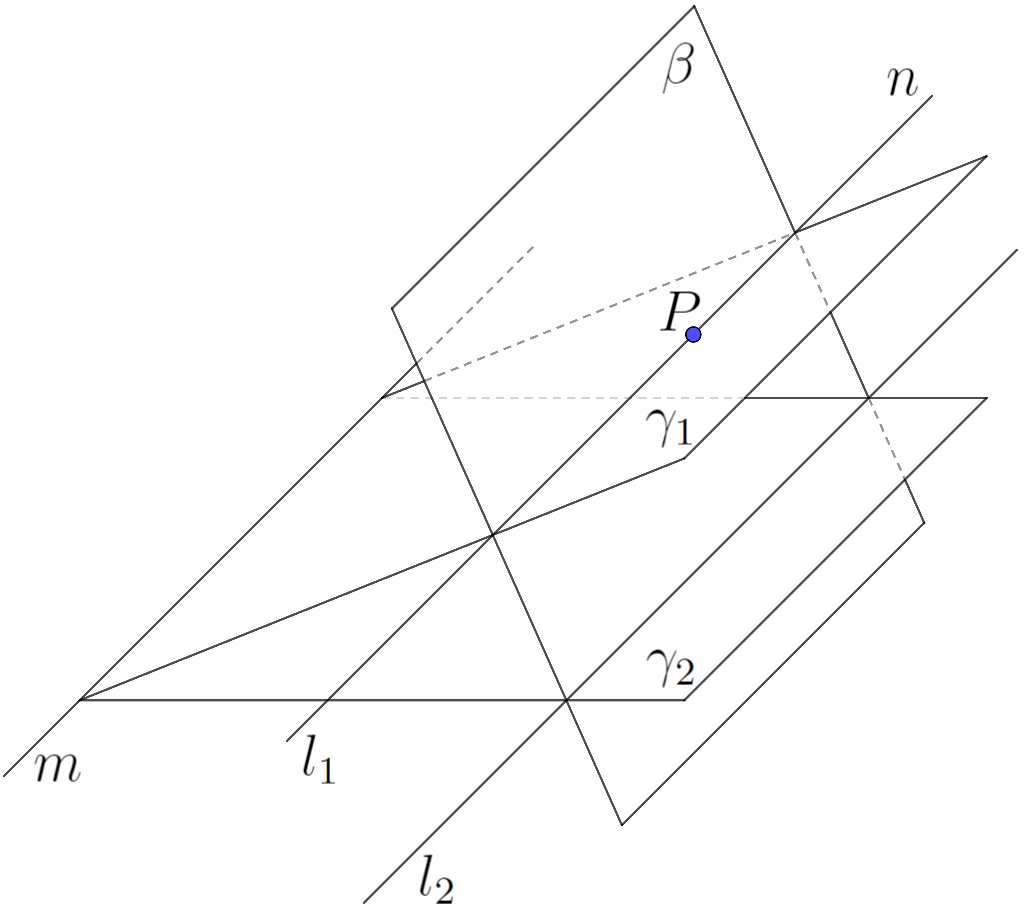
\includegraphics[width=0.5\textwidth]{tu/三平行1.png}
\end{wrapfigure}

有了交面公理,我们可以证明空间中平行直线的递推性质。由于证明繁琐,有些地方把它当作公理引入。
\begin{tm}\label{tm:1-0-10}
    如果直线$l_1,l_2$都平行于直线$m$,那么$l_1,l_2$平行或重合。
\end{tm}
\begin{proof}
    设$l_1,m$确定的平面为$\gamma_1$,$l_2,m$确定的平面为$\gamma_2$。分两种情况讨论:
    

    1. $\gamma_1, \gamma_2$重合。那么$l_1,l_2,m$都在此平面上。根据平面直线的结论,$l_1,l_2$平行或重合。
    
    2. $\gamma_1, \gamma_2$不重合。于是$\gamma_1\cap \gamma_2 = m$。
    取$l_1$上一点$P$,$P$与$l_2$确定平面$\beta$。$l_2\notin\gamma_1$,所以$\beta,\gamma_1$不重合。
    设$\beta\cap\gamma_1 = n$。直觉上,可以想到$n$就是$l_1$,且$n\parallel l_2$,下面来说明这两点。
    
    首先证明$n\parallel l_2$。反设$n$交$l_2$于点$Q$,则$Q\in\gamma_1\cap\gamma_2=m$,
    于是$Q\in m\cap l_2$。这与$m\parallel l_2$矛盾。因此$n\parallel l_2$。
    
    再证明$n\parallel m$。反设$n$交$m$于点$Q$,则过$Q$有$m\parallel l_2$和$n\parallel l_2$,于是$n=m$。
    但$P\in n$,因此$P\in m\cap l_1$,这与$m\parallel l_1$矛盾。因此$n\parallel m$。
    
    $n$与$l_1$都平行于$m$,且有公共点$P$,所以$n = l_1$。所以$l_1\parallel l_2$。
    
\end{proof}

接下来回顾直线与平面的关系。从补充后的平行公理,可以得出直线与平面平行的判定方法:

\begin{tm}\label{tm:1-0-20}
    如果平面$\alpha$中有直线$m$平行于直线$l$,那么$l$平行于平面$\alpha$或在$\alpha$中。
\end{tm}
\begin{proof}
    设直线$l$平行于平面$\alpha$中的某直线$m$。记$l,m$确定的平面为$\beta$。
    则要么$\alpha = \beta$,要么$\alpha\cap\beta = m$。如果$\alpha=\beta$,那么$l\subset\alpha$。
    如果$\alpha\cap\beta = m$,那么由于$l \subset \beta$,$l = \beta \cap l$。于是
    $$\alpha\cap l = \alpha\cap (\beta \cap l) = (\alpha\cap\beta) \cap l = m\cap l = \varnothing. $$
    即$\alpha \parallel l$。
\end{proof}
\begin{tm}\label{tm:1-0-30}
    如果直线$l$与平面$\alpha$平行,那么经过$l$的任意平面,若与$\alpha$相交,其交线也与$l$平行。
\end{tm}
\begin{proof}
    设经过$l$的平面$\gamma$与$\alpha$交于直线$m$。一方面,$m,l$共面;
    另一方面$m\in\alpha$,因此$m,l$无公共点。这说明$m\parallel l$。
\end{proof}

从这些结论可以继续推出:
\begin{tm}\label{tm:1-0-40}
    若直线$l$与平面$\alpha$平行,过$\alpha$中任一点作$l$的平行线$m$,则$m$在平面$\alpha$中。
\end{tm}
\begin{proof}
    若直线$l$与平面$\alpha$平行,设它和$\alpha$中任一点$P$确定的平面为$\beta$,
    则$\beta$与$\alpha$相交。设交线为$m$,则$P\in m$。根据定理\ref{tm:1-0-30},$l\parallel m$。
    这就说明,过$P$而平行于$l$的直线在$\alpha$中。
\end{proof}
\begin{tm}\label{tm:1-0-41}
    直线$l$与直线$m$平行,则过$m$的平面要么与$l$平行,要么经过$l$。
\end{tm}
\begin{proof}
    给定过$m$的平面$\alpha$,$m\subset \alpha$与$l$平行,所以根据定理\ref{tm:1-0-20},
    $l$平行于平面$\alpha$或在$\alpha$中。
\end{proof}

直线与平面的平行关系,也有传递性。
\begin{tm}
    若直线$l_1$与直线$l_2$平行,且与平面$\gamma$平行,则$l_2$与$\gamma$平行或在$\gamma$中。
\end{tm}
\begin{proof}
    $l_1\parallel \gamma$。过$\gamma$中任一点作直线$n\parallel l_1$,则根据定理\ref{tm:1-0-40},
    $n$在$\gamma$中。$n\parallel l_1$,$l_1\parallel l_2$,所以根据定理\ref{tm:1-0-10},$n\parallel l_2$。
    根据定理\ref{tm:1-0-20},$l_2\parallel \gamma$或在$\gamma$中。
\end{proof}

上面提到,两平面要么无公共点,要么相交,要么重合。我们把无公共点的平面称为\textbf{平行平面},也用$\parallel$表记。
平面中,平行公理告诉我们,过直线外一点,恰有一条直线与之平行。空间中的平面,也有类似的结论:
\begin{tm}\label{tm:1-0-50}
    过平面外一点,恰有一平面与之平行。
\end{tm}
\begin{proof}
    设平面$\alpha$外有点$P$。在$\alpha$上选一点$A$,过$A$作两相交直线$l,m$(交点为$A$)。
    根据平行公理,过$P$恰有直线$l', m'$分别与$l,m$平行。$l',m'$相交于点$P$,确定平面$\alpha'$。
    下面证明$\alpha,\alpha'$无公共点,即$\alpha'\parallel\alpha$。

    反设$\alpha,\alpha'$有公共点。由于$P\in\alpha'$在$\alpha$外,两者不重合。
    因此根据交面公理,$\alpha \cap \alpha'$是一条直线,记为$n$。$l,m,n$共面,$l,m$相交,
    因此$l,m$中至少有一条与$n$相交。设$l$与$n$相交,交点为$Q$,则$Q\in n\subset\alpha'$。又因为$l\parallel l'$,$Q\in l$,所以$Q\notin l'$,
    因而在$\alpha'$中,过$Q$可作$l'$的平行线。但这条线在$\alpha'$中,因此不是$l$。这与平行公理矛盾。
        
    因此,$\alpha,\alpha'$无公共点,$\alpha'\parallel\alpha$。
\end{proof}

类似的结论还有:

\begin{tm}\label{tm:1-0-60}
    过平行于平面$\alpha$的一直线$l$,恰有一平面与$\alpha$平行。
\end{tm}
\begin{proof}
在$l$上任取一点$P$,$P\notin \alpha$,因此根据定理\ref{tm:1-0-50},
过$P$恰有一平面$\beta$与$\alpha$平行,只需证明$\beta$经过$l$。
在$\alpha$中任取一点$Q$,则根据定理\ref{tm:1-0-40},过$Q$平行于$l$的直线$m$在$\alpha$中。
$\beta$与$\alpha$平行,也就是说$\beta$与$\alpha$无公共点,
所以$\beta$与$\alpha$的子集$m$也无公共点,即$m\parallel \beta$。过$P$作$m$的平行线,
则根据定理\ref{tm:1-0-40},平行线在$\beta$中。而这条平行线就是$l$,所以$l$在$\beta$中。
这说明过$l$恰有一平面$\beta$与$\alpha$平行。
\end{proof}

从证明中,我们还可以提炼出判定平面平行(或重合)的准则:

\begin{tm}\label{tm:1-0-70}
    给定平面$\gamma_1, \gamma_2$。设$l,m$为$\gamma_1$中的相交直线。
    若$\gamma_2$中有直线$l',m'$分别与$l,m$平行或重合,则平面$\gamma_1, \gamma_2$平行或重合。
\end{tm}
\begin{proof}
    两平面要么相互平行,要么重合,要么相交于一直线。反设$\gamma_1, \gamma_2$相交于直线$n$。

    如果$l=l'$,那么$l\subset \gamma_1\cap\gamma_2$,于是$n=l=l'$。设$m,l$交于点$P$,$m',l'$交于点$Q$。如果$P=Q$,那么$m=m'$,于是$\gamma_1$、$\gamma_2$都是$l,m$确定的平面,$\gamma_1=\gamma_2$。如果$P\neq Q$,那么$P\notin m'$。但$P\in l=n\subset\gamma_2$,因此过$P$作$m'$的平行线,平行线应该在$\gamma_2$中,因此根据平行公理,$m$在$\gamma_2$中。这说明$\gamma_1$、$\gamma_2$都是$l,m$确定的平面,$\gamma_1=\gamma_2$。于是总有两平面重合,矛盾。

    如果$l\parallel l'$,由于$l,m,n$共面,且$l,m$相交,
    因此$l,m$中至少有一条与$n$相交。设$l$与$n$相交,交点为$Q$,则$Q\in n\subset\gamma_2$。又因为$l\parallel l'$,$Q\in l$,所以$Q\notin l'$。
    在$\gamma_2$中,过$Q$可作$l'$的平行线。但这条线在$\gamma_2$中,因此不是$l$。这与平行公理矛盾。

    因此,平面$\gamma_1, \gamma_2$平行或重合。
\end{proof}

平行平面之间,也有类似平行直线的传递性。
\begin{tm}\label{tm:1-0-80}
如果平面$\gamma_1,\gamma_2$都平行于平面$\beta$,那么$\gamma_1,\gamma_2$平行或重合。
\end{tm}
我们先证明一个小结论:
\begin{tm}\label{tm:1-0-90}
    设平面$\gamma_1\parallel \gamma_2$。平面$\beta$与$\gamma_1,\gamma_2$相交于直线$l_1,l_2$,
    则$l_1\parallel l_2$。
\end{tm}
\begin{proof}
    一方面,$l_1,l_2$共面。另一方面,$\gamma_1\parallel \gamma_2$说明$l_1,l_2$无公共点。
    所以$l_1\parallel l_2$。
\end{proof}

从这个结论还可以推出:
如果平面$\gamma_1\parallel \gamma_2$,那么对$\gamma_1$中任意直线,过$\gamma_2$中任一点,作它的平行线,
该平行线都在$\gamma_2$中。

再来证明定理\ref{tm:1-0-80}。
\begin{proof}
    已知平面$\gamma_1,\gamma_2$都平行于平面$\beta$。在$\beta$中找一点$P$,过$P$作相交直线$l,m$。
    在$\gamma_1$中找一点$Q$,过$Q$分别作$l,m$的平行线$l_1,m_1$,则$l_1,m_1$都在$\gamma_1$中。
    它们分别是平面$\gamma_1$与$l,Q$确定的平面$\alpha_1$、平面$\gamma_1$与$m,Q$确定的平面$\alpha_2$的交线。\\
    设$\alpha_1,\alpha_2$分别与$\gamma_2$交于$l_2,m_2$,由于$\gamma_2\parallel \beta$,
    所以根据定理\ref{tm:1-0-30},$l_2\parallel l$,$m_2\parallel m$。因此根据定理\ref{tm:1-0-10},
    $l_2$与$l_1$平行或重合,$m_2$与$m_1$平行或重合。根据定理\ref{tm:1-0-70},$\gamma_1$、$\gamma_2$平行或重合。
\end{proof}

最后,我们还可以得到:
\begin{tm}\label{tm:1-0-100}
    若平面$\gamma_1$与直线$l$平行,且与平面$\gamma_2$平行,则$l$与$\gamma_2$平行或在$\gamma_2$中。
\end{tm}
\begin{proof}
    $l\parallel \gamma_1$,所以过$l$恰有一平面$\beta$与$\gamma_1$平行。如果$\beta=\gamma_2$,
    则$l\subset\gamma_2$。如果$\beta\parallel\gamma_2$,那么$l\parallel \gamma_2$。
    如果$\beta$与$\gamma_2$相交于直线$m$,那么由于$m,l$共面且无公共点,$m\parallel l$。
    于是,根据定理\ref{tm:1-0-20},$l\parallel \gamma_2$或在$\gamma_2$中。
\end{proof}

总结:

我们初步建立了关于空间形状的公理体系,引入了空间中平面的概念,并界定了点、直线和平面的关系:
\begin{enumerate}
    \item 直线和平面都是点的集合。
    \item 直线可能与平面平行、相交,或在平面中。
    \item 直线可能与直线异面、平行、相交、重合。
    \item 平面可能与平面平行、相交、重合。
    \item 直线与直线相交于一点,直线与平面相交于一点,平面与平面相交于一直线。
\end{enumerate}


\begin{sk}
    \mbox{} \\
    \indent 1. 定理\ref{tm:1-0-100} 的证明中,我们讨论了$\beta$与$\gamma_2$相交于直线$m$的情形。实际上$\beta$是否会与$\gamma_2$相交?如何看待这个论证?
\end{sk}

\begin{xt}
    \mbox{} \\
    \indent 1. 证明:如果直线$l$与直线$m$平行,那么过$l$的平面与过$m$的平面要么平行,要么重合,
    要么交于$l,m$之一,要么交于与$l,m$都平行的直线$n$。 
\end{xt}


\section{空间向量}

上一节中,我们使用公理体系讨论空间中的形状。可以看到,使用公理体系讨论虽然严谨,但过于抽象,步骤繁琐。
仅处理点线面的平行关系,就需要大量的篇幅。为此,我们尝试用向量来讨论空间中的形状。

平面中,我们用向量表示点,以及原点到此点的平移。现在我们把向量的概念扩展到空间中。
我们把空间看作集合,记为$\mathbb{V}$,其中的元素称为向量或点。向量满足如下规则:

\begin{enumerate}
    \item 加法结合律:$\forall \,\, \mathbf{a}, \mathbf{b}, \mathbf{c} \in \mathbb{V}$,$\mathbf{a}+ (\mathbf{b} + \mathbf{c}) = (\mathbf{a} + \mathbf{b}) + \mathbf{c}$。
    \item 加法交换律:$\forall \,\, \mathbf{a}, \mathbf{b} \in \mathbb{V}$,$\mathbf{a} + \mathbf{b} = \mathbf{b} + \mathbf{a}$。
    \item 存在零向量:$\forall \,\, \mathbf{a} \in \mathbb{V}$,$\mathbf{a} + \mathbf{0} = \mathbf{a}$。
    \item 放缩和四则运算相容:$\forall \,\, \mathbf{a} \in \mathbb{V}$,$1\cdot \mathbf{a} = \mathbf{a}$。$\forall s, t \in \mathbb{R}$,$(s + t)\cdot\mathbf{a} = (s\cdot\mathbf{a}) + (t\cdot\mathbf{a})$,$(s \cdot t)\cdot \mathbf{a} = s \cdot (t\cdot \mathbf{a})$。
    \item 放缩和平移相容:$\forall \,\, \mathbf{a}, \mathbf{b} \in \mathbb{V}$,$\forall \,\, t \in \mathbb{R}$,$t\cdot(\mathbf{a} + \mathbf{b}) = t\cdot\mathbf{a} + t\cdot\mathbf{b}$。
\end{enumerate}

这个定义与平面向量相同。在此基础上,我们用同样的方式定义直线、线段和射线。
\begin{df}
    过原点的直线是非零向量放缩得到的集合。不过原点的直线是过原点的直线按一点平移得到的集合。
\end{df}
给定非零向量$A = \mathbf{a}$,$ \{t\mathbf{a} \, | \, t\in\mathbb{R}\}$是一条过原点$O$和$A$的直线$OA$,
称为$A$\textbf{引出}的直线,记为$\mathbb{R}\mathbf{a}$。$\mathbf{a}$称为直线的\textbf{方向向量}。
给定向量$B = \mathbf{b}$,$ \{t\mathbf{a}+\mathbf{b} \, | \, t\in\mathbb{R}\}$是一条方向为$\mathbf{a}$且经过$B$的直线,
记为$\mathbb{R}\mathbf{a}+\mathbf{b}$,其中$\mathbb{R}\mathbf{a}$称为它的\textbf{直部};
而$ \{t\mathbf{a}+(1 - t)\mathbf{b} \, | \, t\in\mathbb{R}\}$就是直线$AB$。

给定非零向量$\mathbf{a}$,如果向量$\mathbf{b}$可以通过$\mathbf{a}$放缩得到,
或者说$\mathbf{b}\in \mathbb{R}\mathbf{a}$,就称两者\textbf{共轴}。

类比可以定义线段和射线:给定非零向量$A = \mathbf{a}$和向量$B =\mathbf{b}$,
$ \{(1 - t)\mathbf{a}+t\mathbf{b} \, | \, t\in [0, 1]\}$是线段$AB$,
$ \{(1 - t)\mathbf{a}+t\mathbf{b} \, | \, t \geqslant 0 \}$是射线$AB$。

\begin{figure}[h] 
    % \vspace{-4pt}
    \centering
    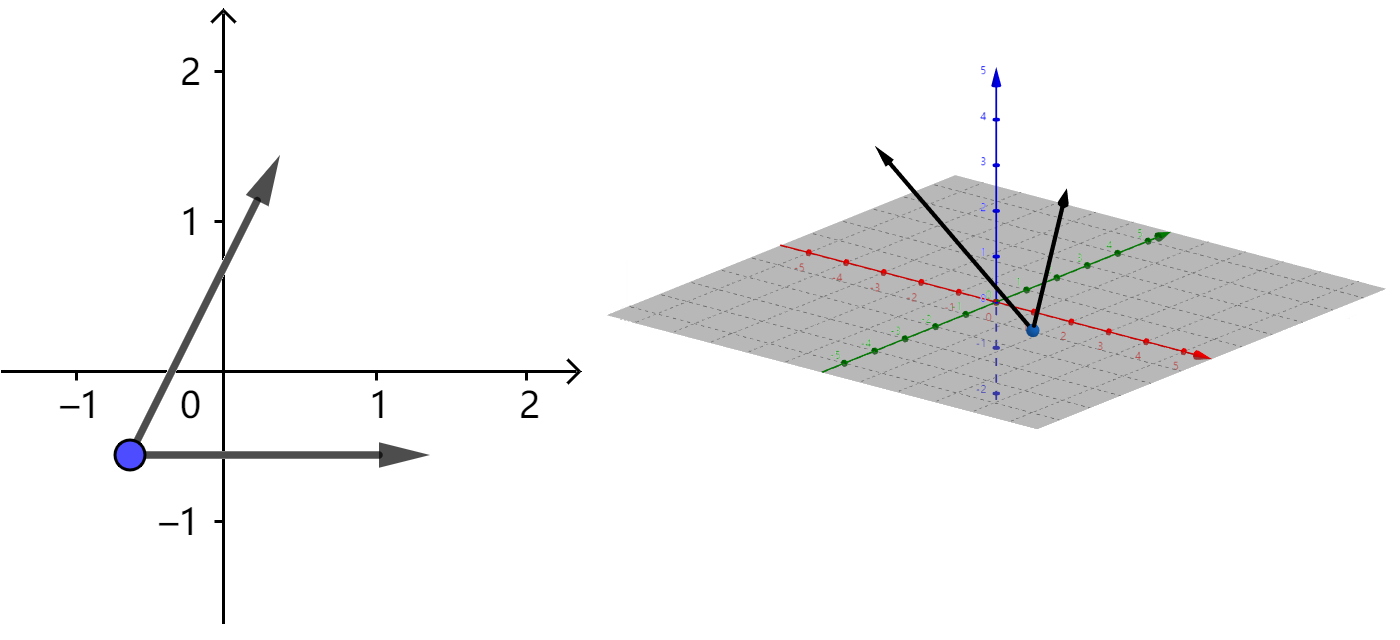
\includegraphics[width=0.8\textwidth]{tu/平面和空间向量1.png}
    \caption*{\texttt{平面和立体空间中的向量}}
\end{figure}

空间向量与平面向量的唯一不同的地方在于,空间向量遵循的不再是平面的根本性质,
而是空间的根本性质。为了描述空间的根本性质,我们先来复习一下直相关的基本性质:
\begin{tm}
    一组向量直无关,则零向量只能用系数全为零的方式表示为它们的直组合。反之亦然。\\
    一组向量直相关,则零向量可以用不同的方式表示为它们的直组合。反之亦然。
\end{tm}

举例来说,单个非零向量总是直无关的,因为非零实数乘以非零向量总得到非零向量。

又如:平面直角坐标系中,令$\mathbf{e}_1=(1,\,\,0)$,$\mathbf{e}_2=(0,\,\,1)$。
如果$A = 2\mathbf{e}_1 - \mathbf{e}_2$,$B = -6\mathbf{e}_1 + 3 \mathbf{e}_2$,那么
$$3A + B = \mathbf{0}.$$
也就是说,选取$t_1 = 3$,$t_2 = 1$,就使得直组合:$t_1A + t_2B$等于零向量。因此,向量$A, B$直相关。

设$A = 2\mathbf{e}_1 - \mathbf{e}_2$,$B = \mathbf{e}_1 + 3 \mathbf{e}_2$,那么对任何$t_1,t_2$,直组合$t_1A + t_2B$可以写为:
\begin{align}
t_1A + t_2B &= t_1 \left( 2\mathbf{e}_1 - \mathbf{e}_2 \right) + t_2 \left( \mathbf{e}_1 + 3 \mathbf{e}_2 \right) \notag \\
&= (2t_1 + t_2) \mathbf{e}_1 + (-t_1 + 3t_2)\mathbf{e}_2.\notag
\end{align}
要使得$t_1A + t_2B$为零向量$(0,\,\,0)$,就要求它的横坐标和纵坐标同时为零。也就是说,$t_1,t_2$应该是二元一次方程组
$$
\left\{
\begin{array}{cl}
  2t_1 + t_2 &= 0 \\
  -t_1 +3t_2 &= 0 \\
\end{array}
\right.
$$
的解。解这个二元一次方程组,得到$t_1=t_2=0$。也就是说,不存在不全为零的实数$t_1, t_2$,
使得直组合$t_1A + t_2B$为零向量。我们说$A, B$直无关。

以上的例子也给出了判断一组向量是否直相关的方法。
我们将“向量的直组合是零向量”
这一条件转化为关于直组合参数的多元一次方程组。如果方程组的解集中有不全为零的解,
这组向量就直相关。如果方程组没有不全为零的解,就说这组向量直无关。

直观来看,两个平面向量直相关和共轴是一回事。$A, B$直相关,
就是说有不全为零的实数$t_1,t_2$使得$t_1A + t_2B$等于零向量。
不妨设$t_1$不为零,那么$A = -\frac{t_2}{t_1}B$,因此$A\in\mathbb{R}B$,即$A, B$共轴。
反之亦然。平面的根本性质告诉我们,存在两个不共轴的向量,也就是说,
不多于两个平面向量,可以直无关。

如果平面中的向量多于两个,平面的根本性质告诉我们,只要其中两个向量$A, B$不共轴,
其余的向量都可以都可以表示成$sA + tB$的形式。
因此,设有平面向量$\mathbf{a}_1, \mathbf{a}_2, \cdots , \mathbf{a}_n$。
如果$\mathbf{a}_1, \mathbf{a}_2$共轴,那么它们直相关,存在$t_1\mathbf{a}_1 + t_2\mathbf{a}_2 = \mathbf{0}$。于是
$$t_1\mathbf{a}_1 + t_2\mathbf{a}_2 + \sum_{i>2}0\cdot\mathbf{a}_i = \mathbf{0}.$$
如果$\mathbf{a}_1, \mathbf{a}_2$不共轴,那么根据平面的根本性质,$\mathbf{a}_3$可以写成:
$$ \mathbf{a}_3 = s\mathbf{a}_1 + t\mathbf{a}_2.$$
于是
$$s\mathbf{a}_1 + t\mathbf{a}_2 - 1\cdot\mathbf{a}_3 + \sum_{i>3}0\cdot\mathbf{a}_i = \mathbf{0}.$$
也就是说,多于两个平面向量总直相关。

这个结论反映了平面向量的本质:可以在平面中选出两个向量,所有向量都可以从它们开始,通过平移、放缩得到。
这两个向量叫作平面的基底。而空间中的点显然不一定在同一个平面里。我们把平面的根本性质替换为\textbf{空间的根本性质}:

\begin{enumerate}
    \item 给定一个非零向量,总能找到另一个向量,使得两者直无关。
    \item 给定两个直无关的向量,总能找到另一个向量,使得三者直无关。
    \item 从直无关的向量$A, B, C$出发,经过放缩、平移,可以得到空间中任何向量。具体来说,
    任何向量都可以表示成$sA + tB + uC$的形式,集合$\{sA + tB + uC \, | \, s, t, u \in\mathbb{R}\}$就是整个空间。
    这样的$A, B, C$称为空间的一组\textbf{基}或\textbf{基底}。
\end{enumerate}

对比平面和空间的根本性质,可以发现,主要的变化是数字“$2$”变成了“$3$”。平面中保证存在两个直无关的向量,
空间中保证存在三个直无关的向量。按照类似的推理,我们可以得到结论:不多于三个空间向量,
可以直无关;多于三个空间向量,总是直相关。我们把这个数字称为\textbf{维数}。平面的维数是$2$,立体空间的维数是$3$。

与平面向量一样,给定基底后,任一空间向量$\mathbf{a}$可以唯一地写成基向量的直组合:
$$ \mathbf{a} = a_x\mathbf{e}_x + a_y\mathbf{e}_y + a_z\mathbf{e}_z.$$
其中$a_x, a_y, a_z$是实数。$(a_x, a_y, a_z)$称为$\mathbf{a}$的\textbf{坐标},
$a_x, a_y, a_z$称为它的\textbf{坐标分量}。

于是我们可以定义立体空间中的平面:
\begin{df}
    过原点的平面是两个直无关的向量通过平移、放缩得到的集合。不过原点的平面是过原点的平面按一点平移得到的集合。
\end{df}

\begin{figure}[h] 
    % \vspace{-4pt}
    \centering
    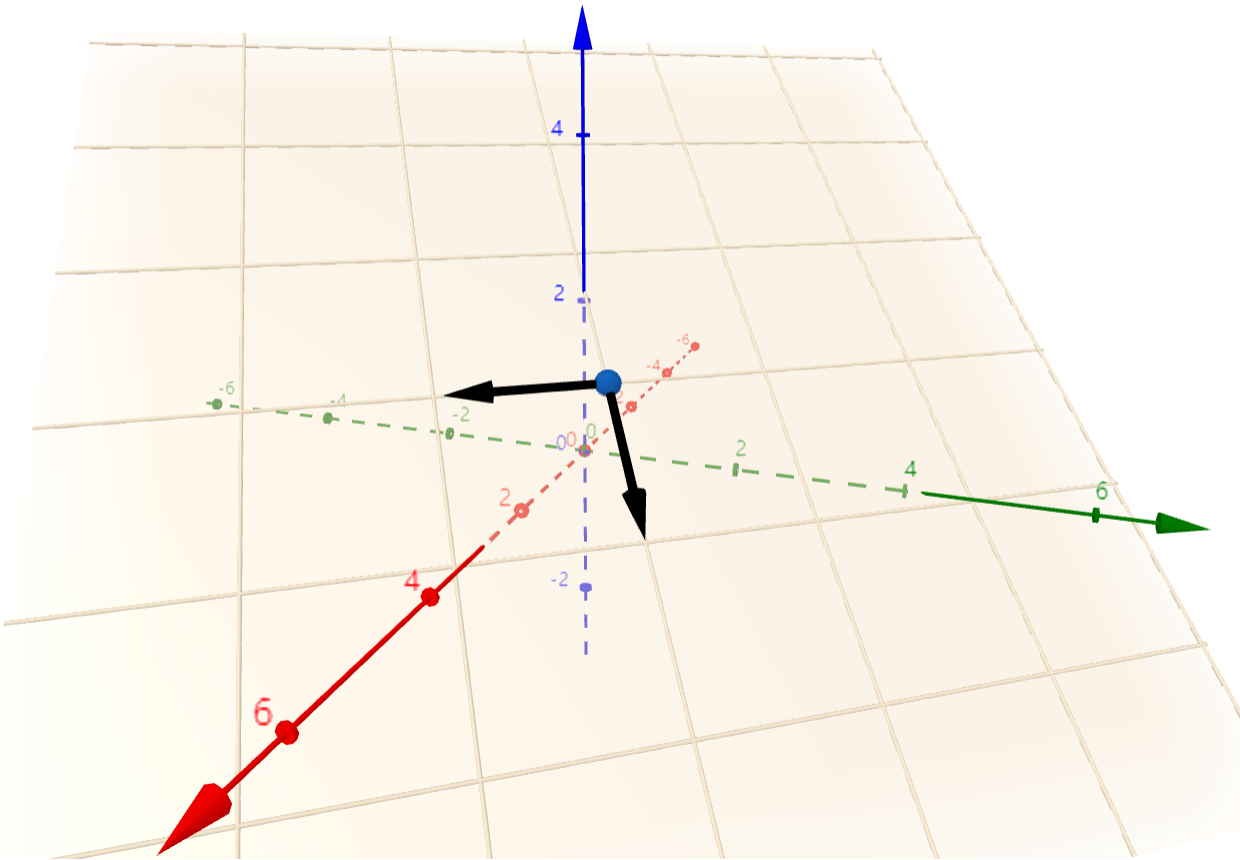
\includegraphics[width=0.5\textwidth]{tu/空间基底1.png}
    \caption*{\texttt{从向量到平面}}
\end{figure}

给定直无关的向量$A = \mathbf{a}, B = \mathbf{b}$,$ \{s\mathbf{a} + t\mathbf{b} \, | \, s, t\in\mathbb{R}\}$是一个过原点$O$和$A, B$的平面$OAB$,
也称为向量$\mathbf{a},\mathbf{b}$\textbf{生成}的平面,简记为$\mathbb{R}\mathbf{a}+\mathbb{R}\mathbf{b}$。
$\mathbf{a},\mathbf{b}$也称为$\mathbb{R}\mathbf{a}+\mathbb{R}\mathbf{b}$的\textbf{生成向量}。

给定向量$C = \mathbf{c}$,$ \{s\mathbf{a}+t\mathbf{b}+\mathbf{c}\, | \, s,t\in\mathbb{R}\}$是一个过$C$的平面,
也记为$\mathbb{R}\mathbf{a}+\mathbb{R}\mathbf{b}+\mathbf{c}$。$\mathbb{R}\mathbf{a}+\mathbb{R}\mathbf{b}$称为它的\textbf{直部}。
而$ \{s\mathbf{a}+t\mathbf{b}+(1 - s - t)\mathbf{c} \, | \, t\in\mathbb{R}\}$就是过$A,B,C$的平面$ABC$。

来看几个具体的例子。选定空间的一组基底$\mathbf{e}_x,\mathbf{e}_y,\mathbf{e}_z$,
我们可以构建坐标系$Oxyz$,其中$x$轴、$y$轴、$z$轴分别是基向量引出的直线$\mathbb{R}\mathbf{e}_x$、
$\mathbb{R}\mathbf{e}_y$、$\mathbb{R}\mathbf{e}_z$。空间中任一点$A$的坐标是$(a_x,a_y,a_z)$。
$x$轴、$y$轴构成平面:
$$ Oxy : \{s\mathbf{e}_x+t\mathbf{e}_y\,|\,s,t\in\mathbb{R}\} = \mathbb{R}\mathbf{e}_x + \mathbb{R}\mathbf{e}_y. $$
$x$轴、$z$轴构成平面:
$$ Oxz : \{s\mathbf{e}_x+t\mathbf{e}_z\,|\,s,t\in\mathbb{R}\} = \mathbb{R}\mathbf{e}_x + \mathbb{R}\mathbf{e}_z. $$
$y$轴、$z$轴构成平面:
$$ Oyz : \{s\mathbf{e}_y+t\mathbf{e}_z\,|\,s,t\in\mathbb{R}\} = \mathbb{R}\mathbf{e}_y + \mathbb{R}\mathbf{e}_z. $$
给出发点$A(3,0,0)$、$B(0,2,0)$、$C(0,0,1)$,则经过它们的平面为:
$$ \{sA+tB+(1 - s - t)C \, | \, t\in\mathbb{R}\} = \{(3s,\,2t,\,1-s-t) \, | \, t\in\mathbb{R}\}. $$

可以验证,这样定义的点、直线、平面符合上一节中的各个公理(见\textbf{附录B})。

\begin{sk}
    \mbox{}  \\
    \indent 1. 张三这样总结空间向量的特性:一个向量平移缩放得到一条直线;两个向量平移缩放可以得到一个平面;
    三个向量平移缩放可以得到整个空间。怎么看待这个说法?\\
    \indent 2. 是否有维数大于$3$的空间?如何在这样的空间中定义向量?这样定义的向量和空间和$2$维、$3$维的向量有什么相同和不同之处?
\end{sk}

\begin{xt}
    \mbox{}  \\
    \indent 1. 判断以下向量是否直相关:\\
    $$
    \begin{array}{ll}
        \mbox{\ding{172}}.\,\,\, (1,2,3),\,\,\,(4,5,6), \,\,\,(7,8,9) \quad & \mbox{\ding{173}}.\,\,\, (1,0,-1),\,\,\, (1,2,0) \,\,\,(-2,2,3)  \\
        \mbox{\ding{174}}.\,\,\, (2,1,-1), \,\,\, (2,-5,-7), \,\,\,(1,-1,-2) \quad & \mbox{\ding{175}}.\,\,\, (a,0,b),\,\,\, (b,-a,0) \,\,\,(a,b,0) 
    \end{array}
    $$
    \indent 2. 已知直线$\mathbb{R}\mathbf{a}+\mathbf{b}$和直线外一点$P$,如何表示它们确定的平面?\\
    \indent 3. 一直两条直线相交于点$P$,方向向量分别是$\mathbf{a},\mathbf{b}$,如何表示这两条直线,以及它们确定的平面?\\
    \indent 4. 设有向量$\mathbf{a}=(0,1,1)$、$\mathbf{b}=(2,-1,0)$、$\mathbf{c}=(1,1,-1)$。
    平面$\gamma = \{s\mathbf{a} + t\mathbf{b} + \mathbf{c} \, | \, s,t,\in\mathbb{R}\}$。\\
    \indent 4.1. 判断点$(5,1,-2)$、$(3,2,1)$、$(0,5,0)$是否在平面上。\\
    \indent 4.2. 点$(1,0,0)+u(0,-1,3)$在平面$\gamma$中,求它的坐标。\\
    \indent 4.3. 直线$l$在平面$\gamma$中,证明:它的方向向量是$\mathbf{a},\mathbf{b}$的直组合。
\end{xt}

\section{角度和长度}
我们可以通过向量引进空间中角度、长度和距离的概念。和平面中一样,
我们选定空间的一组基底$\mathbf{e}_x,\mathbf{e}_y,\mathbf{e}_z$,然后定义內积:
$$
\begin{array}{c}
    \forall  A = a_x\mathbf{e}_x+a_y\mathbf{e}_y+a_z\mathbf{e}_z,\,\,B = b_x\mathbf{e}_x+b_y\mathbf{e}_y+b_z\mathbf{e}_z, \notag \\
     A\cdot B = a_xb_x + a_yb_y + a_zb_z. \notag
\end{array}
$$ 
如果向量$A,B$的內积等于$0$,就说它们垂直。我们定义向量$A$的长度为
$$\|A\| = \sqrt{A\cdot A} = \sqrt{a_x^2 + a_y^2 + a_z^2},$$
长度为$1$的向量称为\textbf{单位向量}。任何非零向量除以自己的长度,都得到一个与自己共轴的单位向量。
我们把这个操作称为\textbf{向量的归一}。

两点$A,B$之间的距离是:
$$\|A-B\| = \sqrt{(A - B)\cdot(A-B)} = \sqrt{(a_x - b_x)^2 + (a_y-b_y)^2 + (a_z-b_z)^2}. $$

平面向量的内积,小于等于长度之积。空间向量也有类似的性质:
\begin{align}
    &(a_x^2 + a_y^2 + a_z^2)(b_x^2 + b_y^2 + b_z^2) \notag \\
    =\,\,& (a_xb_x + a_yb_y + a_zb_z)^2 + (a_xb_y - a_yb_x)^2 + (a_xb_z - a_zb_x)^2 + (a_yb_z - a_zb_y)^2 \notag \\
    \geqslant\,\,& (a_xb_x + a_yb_y + a_zb_z)^2 \notag 
\end{align}
这个不等式也称为\textbf{内积不等式}。由此,类比平面向量,我们可以定义\textbf{空间向量的夹角}:
$$ \cos \angle AOB = \frac{a_xb_x + a_yb_y + a_zb_z}{\sqrt{(a_x^2 + a_y^2 + a_z^2)(b_x^2 + b_y^2 + b_z^2)}}$$
直线是非零向量放缩的结果,所以,可以定义空间中两条直线的夹角为它们的方向向量的夹角。

向量$A,B$垂直时,$\cos \angle AOB = 0$,即夹角为$90^\circ$。
向量夹角为$0^\circ$、$180^\circ$时,两向量共轴,两直线同向或反向。
要注意的是,空间中,我们无法定义两向量夹角的方向。

\begin{sk}
    \mbox{} \\
    \indent 1. 内积不等式取等号的条件是什么?如何从直观上理解?\\
    \indent 2. 平面中,向量夹角的正弦与向量长度的乘积对应着向量的面积。
    立体空间中,是否可以作类似的定义?如何从直观上理解?
\end{sk}

\begin{xt}
    \mbox{} \\
    \indent 1. 已知向量$A(-1, 3, 1)$、$B(1, 2, 0)$,求它们的长度、内积和夹角。它们是否垂直?\\
    \indent 2. 已知向量$A(-2.4, 0, 1)$、$B(0.5, 1, 1.2)$,求它们的长度、内积和夹角。它们是否垂直?\\
    \indent 3. 已知直线$l_1: \mathbb{R}(1,2,-2.5) + (0,-1,-1)$、$l_2: \mathbb{R}(2,0,0.8) + (-2.5,1.1,1.7)$,
    求两直线的夹角。它们是否垂直?是否有公共点?\\
    \indent 4. 已知向量$A(2, 0, 1)$,求与$A$夹角为$60^\circ$的单位向量。
\end{xt}

\section{垂直和投影}

通过内积,我们已经定义了空间向量以及直线间的垂直关系。
下面来看直线与平面的垂直关系。直线与平面垂直,是直线与平面相交的特殊情形。
\begin{df}\label{df:1-3-10}
    给定直线$l$和平面$\gamma$,如果$\gamma$中任意直线都与$l$垂直,就说平面$\gamma$与$l$垂直。
\end{df}
用向量的语言来说,直线垂直于平面,即垂直于它的直部中的所有向量。

给定了直线和平面,如何判定它们垂直呢?我们从以下基本性质出发:
\begin{tm}\label{tm:1-3-10}
    如果向量$\mathbf{a}$垂直于另两个向量$\mathbf{u},\mathbf{v}$,
    那么$\mathbf{a}$也与$\mathbf{u},\mathbf{v}$的任何直组合垂直。
\end{tm}
\begin{proof}
    如果$\mathbf{a}\perp \mathbf{u}$、$\mathbf{a}\perp \mathbf{v}$,按照定义,
    $$ \mathbf{a}\cdot \mathbf{u} = 0, \quad \mathbf{a}\cdot \mathbf{v} = 0. $$
    于是,$\forall s, t\in\mathbb{R}$,
    \begin{align}
        \mathbf{a}\cdot (s\mathbf{u} + t\mathbf{v}) = s\mathbf{a}\cdot \mathbf{u} + t\mathbf{a}\cdot \mathbf{v} = 0. \notag
    \end{align}
\end{proof}

给定直线$l$和平面$\gamma$中两条相交直线。设$l$的方向向量为$\mathbf{a}$,
两条相交直线相交于点$P$,方向向量为直无关的向量:$\mathbf{u},\mathbf{v}$,那么$\gamma$可以表示成
$$ \gamma = \{s\mathbf{u} + t\mathbf{v} + P \, | \, s,t\in\mathbb{R}\} = \mathbb{R}\mathbf{u} + \mathbb{R}\mathbf{v} + P. $$
因此,$\gamma$中任一直线的方向向量总是$\mathbf{u},\mathbf{v}$的直组合。
如果$\mathbf{a}$垂直于$\mathbf{u},\mathbf{v}$,那么根据定理\ref{tm:1-3-10},
$l$垂直于$\gamma$中任一直线,因而垂直于平面$\gamma$。我们可以把这个结论总结为:
\begin{tm}\label{tm:1-3-20}
    直线与平面垂直,当且仅当它垂直于平面中两条相交直线。
\end{tm}
接下来我们自然要问:给定了平面,是否有与它垂直的直线呢?

从以上的讨论来看,关键是找到与平面中两个直无关的向量都垂直的向量。

首先来看平面中的情况。给定非零平面向量$A$,是否有(非零)向量与它垂直?
根据平面的根本性质,总存在与$A$不共轴的向量$B$。但$B$不一定与$A$垂直。
下面我们从$B$出发,找一个与$A$垂直的非零向量。

直观上,向量$A,B$确定一个平行四边形,我们将它沿着$A$的方向“平推”,可以把它“扶正”,变成一个矩形。
矩形的另一边就和$A$垂直了。把这个想法用向量表示,我们考虑向量$B' = B + uA$,其中$u\in\mathbb{R}$是系数。
$B'$是$B$沿$A$方向移动得到的。我们希望$B'\perp A$,即内积为$0$:
$$ A\cdot B = A\cdot (B + uA) = 0$$
解得$u = -\frac{A\cdot B}{A\cdot A}$。
这样我们就找到了垂直于$A$的非零向量$B' = B -\frac{A\cdot B}{A\cdot A}A$。

直观来看,过$B$作直线$OA$的垂线,设垂足为$P$,则$\frac{A\cdot B}{A\cdot A}A$就是向量$OP$。
如果想象$OA$为水平线,线段$OB$是一根杆子,那么线段$OP$可以看成$OB$在竖直照射的阳光下的影子。
我们把向量$\vv{OP}$称为向量$\vv{OB}$在直线$OA$上的投影。严格的定义如下:
\begin{df}\label{df:1-3-20}
    给定向量$\mathbf{a}$和向量集合$S$。如果向量$\mathbf{y}\in S$使得$\mathbf{a} - \mathbf{y}$垂直于
    $S$中所有向量,就说$\mathbf{y}$是$\mathbf{a}$在$S$中的\textbf{投影},
    $\mathbf{a} - \mathbf{y}$是$\mathbf{a}$关于$S$的\textbf{修正}。
\end{df}
按照严格的定义,向量$\vv{OP}$就是向量$\vv{OB}$在直线$OA$中的投影。
从$\vv{OB}$中减去它在直线$OA$上的投影,得到垂直于$\vv{OA}$的向量(或者说关于直线$OA$的修正),
这种方法叫做\textbf{消影法}。

我们可以进一步将$A$和$B'$分别归一,就得到两个相互垂直的单位向量。
我们把这样两个向量称为平面的\textbf{正交归一基}。注意到$A,B$是平面的一组基底。
从$A,B$出发得到正交归一基,这个过程称为\textbf{基底的正交归一}。

空间的根本性质告诉我们,给定两个直无关的向量$A,B$,总有向量$C$使得$A,B,C$为空间的基底。
我们尝试用消影法将它正交归一,得到空间的正交归一基$A_1,B_1,\mathbf{n}$,然后证明$\mathbf{n}$与$A,B$垂直。

\begin{figure}[h] 
    % \vspace{-4pt}
    \centering
    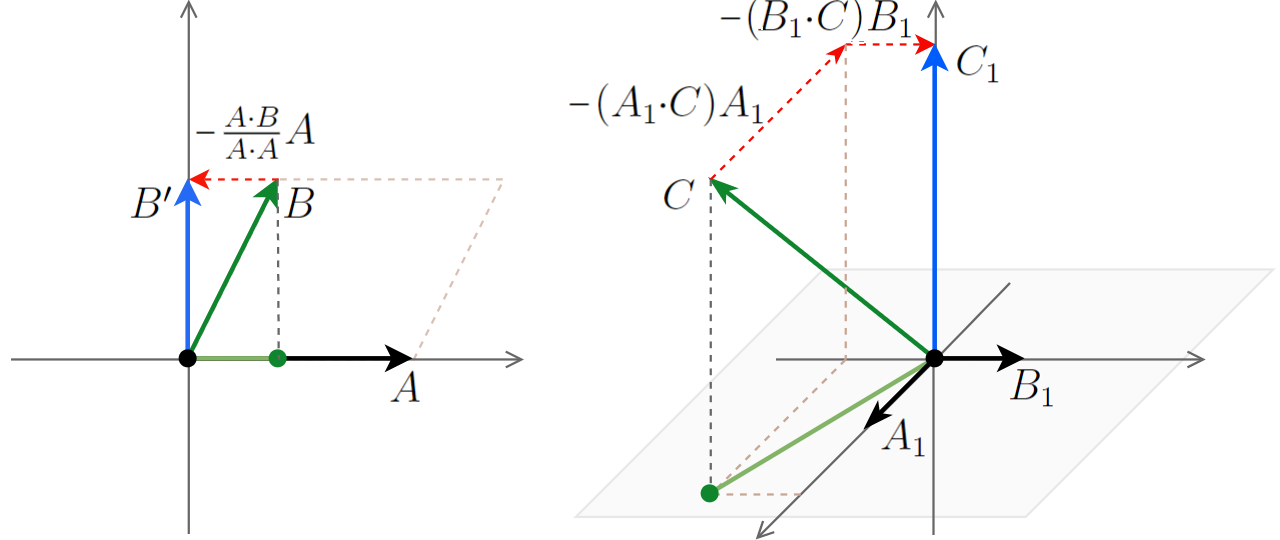
\includegraphics[width=0.8\textwidth]{tu/消影法1.png}
    \caption*{\texttt{平面和立体空间中的消影法}}
\end{figure}

根据已知条件,$A,B$确定一个平面$\gamma$,而且是平面$\gamma$的基底。用消影法将$A,B$正交归一,
得到平面$\gamma$的正交归一基$A_1,B_1$。然后再次使用消影法。这次我们要消去$C$在平面$\gamma$中的投影。
考虑向量$C_1=C+uA_1+vB_1$,其中$u,v$是未知系数。
我们希望$C_1$与$A_1,B_1$垂直。分别计算内积$A_1\cdot C_1$、$B_1\cdot C_1$,两者都应当等于$0$。
于是得到关于$u,v$的方程组:
$$
    \left\{
    \begin{array}{cl}
    A_1\cdot C + u\|A_1\|^2 + vA_1\cdot B_1 &= 0 \\
    B_1\cdot C + uA_1\cdot B_1 + v\|B_1\|^2 &= 0 \\
    \end{array}
    \right.
$$
$A_1,B_1$为正交归一基,所以$A_1\cdot B_1 = 0$,$\|A_1\|^2 = \|B_1\|^2 = 1$。因而解得:
$$
    \left\{
    \begin{array}{cl}
    u &= -A_1\cdot C \\
    v &= -B_1\cdot C \\
    \end{array}
    \right.
$$
这样我们就得到了与$A_1,B_1$都垂直的向量
$$ C_1 = C - (A_1\cdot C)A_1 - (B_1\cdot C)B_1. $$
它是从$C$中去掉它在平面$\gamma$中的投影$(A_1\cdot C)A_1 + (B_1\cdot C)B_1$得到的。
将它归一,就得到垂直于$A_1,B_1$的单位向量:$\mathbf{n} = \frac{C_1}{\|C_1\|}$ 。
于是我们得到了空间的正交归一基:$A_1,B_1,\mathbf{n}$。

$A_1,B_1$是$A,B$确定的平面的正交归一基,所以$A,B$可以表示为$A_1,B_1$的直组合。
$\mathbf{n}$与$A_1,B_1$都垂直,因此也垂直于它们的直组合$A,B$。
于是我们得到结论:
\begin{tm}\label{tm:1-3-30}
    给定两个直无关的向量$A,B$,存在单位向量$\mathbf{n}$与它们都垂直。
\end{tm}
任何平面总由两个直无关的向量确定。设平面$\gamma = \mathbb{R}A + \mathbb{R}B + C$,
则存在单位向量$\mathbf{n}$与$A,B$都垂直。我们称单位向量$\mathbf{n}$为$\gamma$的\textbf{法向量}\footnote{约定平面的法向量为单位向量,可以方便讨论。类似地,以下也约定直线的方向向量为单位向量。}。
以法向量为方向向量的直线,就与平面垂直。这样,我们就找到了与平面垂直的直线。

与同一平面垂直的直线有什么共同特征呢?
从前面的推导还可以得出:所有与$A,B$都垂直的向量共轴。

在前面的推导中,我们知道$A_1,B_1,\mathbf{n}$是空间的基底。因此,空间中任何向量$\mathbf{w}$可以分解为:
$$ \mathbf{w} = w_A A_1 + w_B B_1 + w_n \mathbf{n}. $$
如果它与$A,B$都垂直,那么也垂直于它们的直组合:$A_1,B_1$。计算它与$A_1,B_1$的內积,得到:
\begin{align}
    0 = \mathbf{w}\cdot A_1  = w_A\|A_1\|^2 = w_A, \notag \\
    0 = \mathbf{w}\cdot B_1  = w_B\|B_1\|^2 = w_B, \notag 
\end{align}
这说明$\mathbf{w} = w_n \mathbf{n}$,与$\mathbf{n}$共轴。
或者说,所有与$A,B$都垂直的向量的集合是$\mathbb{R}\mathbf{n}$。

所有与$A,B$都垂直的向量共轴,因此都在$\mathbb{R}\mathbf{n}$上。
因此,垂直于$A,B$确定的平面的直线,其方向向量总在$\mathbb{R}\mathbf{n}$上。
换句话说,
\begin{tm}\label{tm:1-3-40}
    垂直于同一平面的直线平行或重合。
\end{tm}
给定空间中一点$P$和平面$\gamma$,在$\gamma$上任取一点$O$,引出两个直无关的向量$OA,OB$,
于是有单位向量$\mathbf{n}$与它们都垂直,于是$\mathbb{R}\mathbf{n} + P$是过$P$且垂直于$\gamma$的直线。
另一方面,如果过$P$的直线$\mathbb{R}\mathbf{m} + P$垂直于$\gamma$,
那么它$\mathbf{m}$垂直于$\vv{OA},\vv{OB}$。于是$\mathbf{n}$与$\mathbf{m}$共轴,
$\mathbb{R}\mathbf{m} + P$就是直线$\mathbb{R}\mathbf{n} + P$。也就是说,
\begin{tm}\label{tm:1-3-50}
    过一点恰有一条直线与给定平面垂直。
\end{tm}
我们把过空间中一点到给定平面垂直的唯一直线称为点到这个平面的\textbf{垂线},垂线与平面的交点称为\textbf{垂足}。
垂足也称为\textbf{点在平面中的投影}。

使用法向量和投影,我们可以定义向量和平面的交角。
考虑法向量为$\mathbf{n}$的(过原点的)平面$\gamma$和平面外向量$A$,
我们定义向量$A$与平面$\gamma$的交角为$A$和平面法向量$\mathbf{n}$的交角的余角。
这是因为平面的法向量应该看作垂直于平面的标志。因此类比平面中向量和两垂直向量的角度关系,
空间中向量和平面及其法向量的交角应该互为余角。

直观来看,设$A$在$\gamma$中的投影为$P$,
则$\triangle OAP$是直角三角形,$\angle APO$是直角。$\vv{OP}$是$\vv{OA}$在$\gamma$中的投影,
$\vv{PA}$是$\vv{OA}$关于$\gamma$的修正。因此,$\angle OAP$是$A$和$\mathbf{n}$的交角,
它的余角$\angle AOP$就是$A$和平面的交角。

直线和平面的交角,定义为它的方向向量和平面的交角。

除了点和向量,也可以定义\textbf{直线在平面中的投影}。给定直线$l$,
$l$中的点在平面中投影的集合,就构成$l$在平面中的投影。
\begin{tm}\label{tm:1-3-55}
    如果直线垂直于平面,那么它在平面中的投影是一个点,即直线和平面的交点。
    如果直线不垂直于平面,那么它在平面中的投影是一条直线。    
\end{tm}
\begin{proof}
    设有直线$l$和平面$\gamma$。$l$与$\gamma$或相交、或平行,或在$\gamma$中。设$m$为$l$在平面中的投影。

    如果$l$在$\gamma$中,那么$m=l$。

    如果$l$与$\gamma$交于点$P$,那么$P$就是它自己在$\gamma$的垂足,因此$P\in m$。
    设$l=\mathbb{R}\mathbf{v}+P$,平面法向量为$\mathbf{n}$。
    对$l$中另一点$Q = t\mathbf{v}+P$,作$Q$到$\gamma$的垂线,垂足为$R$,则$R\in m$。
    直线$QR\perp\gamma$,所以$QR\perp PR$,因此
    $$ \vv{PR}\cdot\vv{QR} = 0.$$
    向量$\vv{PR} = \vv{PQ} + \vv{QR}$,设$\vv{QR} = s\mathbf{n}$,则
    $$ 0 = (\vv{PQ} + \vv{QR})\cdot\vv{QR} = (Q - P) \cdot\vv{QR} + \|\vv{QR}\|^2 = st\mathbf{v}\cdot\mathbf{n} + s^2. $$
    解得$s=0$或$s = -t\mathbf{v}\cdot\mathbf{n}$。
    
    $s=0$表示$Q=R\in \gamma\cap l$,于是$Q=P$,舍弃。
    于是$s = -t\mathbf{v}\cdot\mathbf{n}$。
    $$\vv{PR} = \vv{PQ} + \vv{QR} = t\mathbf{v} -t(\mathbf{v}\cdot\mathbf{n})\mathbf{n} = t(\mathbf{v} - (\mathbf{v}\cdot\mathbf{n})\mathbf{n}). $$
    
    如果$\mathbf{v}, \mathbf{n}$共轴,那么$(\mathbf{v}\cdot\mathbf{n})\mathbf{n} = \mathbf{v}$。
    于是$\vv{PR} = \mathbf{0}$,$P = R$。这说明如果直线垂直于平面,则直线上的点的投影总是直线与平面的交点$P$。

    如果$\mathbf{v},\mathbf{n}$不共轴,那么$R$在直线$f:\mathbb{R}(\mathbf{v} - (\mathbf{v}\cdot\mathbf{n})\mathbf{n}) + P$上。
    具体来说,$l$上的点和它的投影点是直线$l$到$f$的一一对应:
    $$ t\mathbf{v}+P \mapsto t(\mathbf{v} - (\mathbf{v}\cdot\mathbf{n})\mathbf{n}) + P.$$
    因此,$l$的投影$m$就是直线$f$。
    
\end{proof}

以下定理说明了直线和它在平面中的投影的关系。
\begin{tm}{\textbf{三垂线定理}}\label{tm:1-3-57}
    设直线$l$在平面$\gamma$中的投影为直线$m$,那么$l$垂直于平面$\gamma$中直线$f$,当且仅当$m$垂直于$f$。
\end{tm}
\begin{proof}
    设$l=\mathbb{R}\mathbf{v}+P$,平面法向量为$\mathbf{n}$。
    根据定理\ref{tm:1-3-55},投影直线$m$可以表示为
    $$m = \mathbb{R}(\mathbf{v} - (\mathbf{v}\cdot\mathbf{n})\mathbf{n}) + P.$$
    设$\gamma$中直线$f$的方向向量为$\mathbf{u}$。则$\mathbf{u}$垂直于平面的法向量$\mathbf{n}$。
    而$l$与$m$的方向向量相差$(\mathbf{v}\cdot\mathbf{n})\mathbf{n}$。
    如果计算它们与$\mathbf{u}$的内积,会发现:
    $$ (\mathbf{v} - (\mathbf{v}\cdot\mathbf{n})\mathbf{n})\cdot \mathbf{u} = \mathbf{v} \cdot \mathbf{u} - (\mathbf{v}\cdot\mathbf{n})\mathbf{n} \cdot \mathbf{u} = \mathbf{v} \cdot \mathbf{u}. $$
    两内积相等,它们同时等于$0$或不等于$0$。
    所以,如果$\mathbf{v} \perp \mathbf{u}$,那么$\mathbf{v} - (\mathbf{v}\cdot\mathbf{n})\mathbf{n} \perp \mathbf{u}$。
    反之,如果$\mathbf{v} - (\mathbf{v}\cdot\mathbf{n})\mathbf{n} \perp \mathbf{u}$,那么$\mathbf{v} \perp \mathbf{u}$。
    对于直线来说,这就说明$l$垂直于直线$f$,当且仅当$m$垂直于$f$。
\end{proof}

\begin{et}\label{et:1-3-10}
    平面中有平行四边形$ABCD$,过$A$作直线$AM$垂直于平面。$M$为直线上一点。
    $|BC|$满足什么条件的时候,直线$CM$垂直于$BD$?
\end{et}
\begin{so}
    在水平面上画出平行四边形$ABCD$,作出直线$AM$,可以看到,直线$AC$就是直线$CM$在平面中的投影。
    因此,根据三垂线定理,$CM$垂直于$BD$当且仅当$AC$垂直于$BD$,即$ABCD$为菱形。也就是说,
    当$|BC|=|AB|$的时候,直线$CM$垂直于$BD$,否则直线$CM$不垂直于$BD$。
\end{so}

\begin{wrapfigure}[6]{r}{0.42\textwidth} %this figure will be at the right
    \vspace{-45pt}
    \flushright
    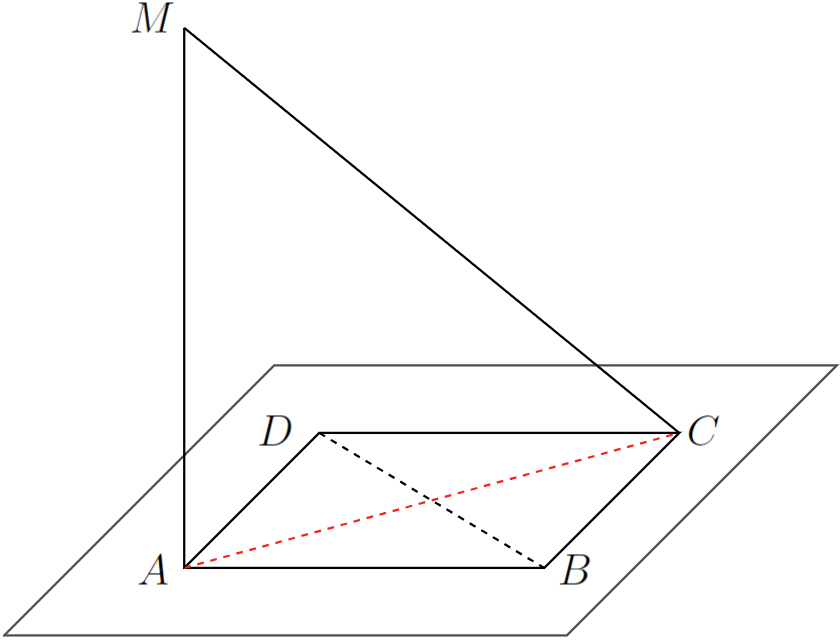
\includegraphics[width=0.4\textwidth]{tu/垂线例10.png}
    \caption*{\texttt{例题}\ref{et:1-3-10}}
\end{wrapfigure}

给定平面,总有与它垂直的直线。反过来,给定一条直线,是否有与它垂直的平面呢?设直线的方向向量为$\mathbf{n}$,
我们来看与它垂直的向量有什么共同特征。
\begin{tm}\label{tm:1-3-60}
    所有与非零向量$\mathbf{n}$垂直的向量构成一个过原点的平面。    
\end{tm}
\begin{proof}
设$\mathbf{n} = (n_x, n_y, n_z)$是非零向量,所以$n_x, n_y, n_z$不全为零。
设$n_x\neq 0$,则向量$P_1(-n_y, n_x, 0)$和$P_2(-n_z, 0, n_x)$都垂直于$\mathbf{n}$。
容易验证$P_1,P_2$直无关,因此它们确定的平面$\gamma$垂直于$\mathbf{n}$。

另一方面,设$P$与非零向量$\mathbf{n}$垂直,下面证明$P$在平面$\gamma$中。

可以验证$P_1, P_2, \mathbf{n}$直无关,因此是空间的一组基底。用消影法将它正交归一,
得到正交归一基$(Q_1, Q_2,\mathbf{m})$,其中$Q_1,Q_2$是$P_1, P_2$正交归一的结果,
是平面$\gamma$的正交归一基,$\mathbf{m}$是平面$\gamma$的法向量,因此$\mathbf{m}$、$\mathbf{n}$共轴。
将$P$在$Q_1, Q_2,\mathbf{m}$上分解:
$$ P = p_1Q_1 + p_2Q_2 + p_m\mathbf{m}.$$
$P$垂直于$\mathbf{n}$,因此也垂直于$\mathbf{m}$。于是$\mathbf{m}\cdot P = 0$,
即$p_m = 0$。因此$P = p_1Q_1 + p_2Q_2$在平面$\gamma$中。
综上所述,所有与非零向量$\mathbf{n}$垂直的向量构成过原点的平面$\gamma$。

\end{proof}

给定一条直线$l:\mathbb{R}\mathbf{a} + \mathbf{b}$及一点$P$,
与$\mathbf{a}$垂直的向量构成一个过原点的平面。
把该平面按$P$平移,就得到一个过$P$的平面。也就是说:
\begin{tm}\label{tm:1-3-70}
    过一点恰有一个平面与给定直线垂直。
\end{tm}

过空间的每一点,恰有一个平面与给定直线垂直。这些垂直于同一直线的平面,有什么特征呢?
\begin{tm}\label{tm:1-3-80}
    垂直于同一直线的平面,相互平行或重合。
\end{tm}
\begin{proof}
    设平面$\gamma_1,\gamma_2$与直线$l$垂直,与$l$分别交于点$P_1,P_2$。过$P_1$在$\gamma_1$中作两条直线$m_1,m_2$,
    过$P_2$作$m_1$的平行线$n_1$,$n_1\perp l$,因此$n_1$在$\gamma_2$中。
    同理,过$P_2$作$m_2$的平行线$n_2$,$n_2$在$\gamma_2$中。
    因此根据定理\ref{tm:1-0-70},$\gamma_1$与$\gamma_2$平行或重合。
\end{proof}

设非零向量$\mathbf{n} = (n_x, n_y, n_z)$,与它垂直的向量的集合,就是以下方程的解集。
$$ n_xx + n_yy + n_zz = 0. $$
任何过原点的平面,都有法向量,于是总可以写成三元一次方程的解集。
因此,过原点的平面,可以用一个三元一次方程定义。

不过原点的平面,可以看作过原点平面按同一向量平移得到。如果过原点平面上的点满足方程
$$ n_xx + n_yy + n_zz = 0, $$
那么按向量$B(x_b, y_b,z_b)$平移之后得到的点就满足方程:
$$ \mbox{}\qquad\qquad n_x(x - x_b) + n_y(y - y_b) + n_z(z - z_b) = 0. \quad\quad (*)$$
因此,任何平面总是某个三元一次方程的解集。反之,任何三元一次方程$ax+by+cz+d = 0$总能写成
$(*)$的形式,于是解集为某个平面。我们将$ax+by+cz+d = 0$称为\textbf{平面的一般式},将$(*)$称为\textbf{平面的点法式},
即经过$B(x_b, y_b,z_b)$且垂直于向量$\mathbf{n} = (n_x, n_y, n_z)$。

三元一次方程的解集是平面,因此,我们也用它来定义平面。
比如,$x$轴和$y$轴所在平面$Oxy$可以用方程$z = 0$定义,过点$(-2,10,3)$并与它平行的平面可以用$z = 3$定义。	

用方程来定义平面,可以得出更多结论。
比如,考虑到空间中两点$P_1(x_1, y_1, z_1)$和$P_2(x_2, y_2, z_2)$相等的点$P(x,y,z)$,这样的点满足方程:
$$ (x - x_1)^2 + (y - y_1)^2 + (z - z_1)^2 = (x - x_2)^2 + (y - y_2)^2 + (z - z_2)^2. $$
方程两边消去$x^2 + y^2 + z^2$,得到关于$x,y,z$的三元一次方程:
$$ 2(x_1-x_2)x + 2(y_1-y_2)y + 2(z_1-z_2)z = x_1^2+y_1^2+z_1^2 - x_2^2-y_2^2-z_2^2. $$
因此,到两点距离相等的点构成一个平面,称为这两点的\textbf{垂直平分面}。


\begin{et}\label{et:1-3-20}
    平面$\gamma$中有直角梯形$ABCD$,$AB \perp BC$,$BC \perp CD$,$|AB|= 2$、$|BC| = 1$、$|CD| = 4$。
    平面外的点$P$满足$PA \perp AB$。\\
    证明:$|PC| = |PD|$。
    % 2. 已知$|PA| = 1$,求$PAC$与$PCD$夹角的最大值。
\end{et}
\begin{so}
    $PA \perp AB$,$AB \parallel CD$,所以$PA \perp CD$。根据勾股定理,$|AC| = \sqrt{5} = |AD|$,所以$\triangle ACD$是等腰三角形。
    记$CD$中点为$M$,则$AM \perp CD$,所以$CD \perp PAM$。于是$CD \perp PM$。因此,根据勾股定理,
    $$ |PC| = \sqrt{|PM|^2 + |CM|^2} = \sqrt{|PM|^2 + |DM|^2} = |PD|.$$
    对平面$PAM$中任意点$Q$,连接$QM$,可以用这个方法证明$|QC| = |QD|$。也就是说,平面$PAM$是$C$、$D$的垂直平分面。\\
    % 2. 以$M$为原点建立空间直角坐标系,以$\vv{CD}$方向的单位向量为$\mathbf{e}_x$,
    % 以$\vv{CB}$方向的单位向量为$\mathbf{e}_y$\footnote{$\mathbf{e}_z$的取法有两种可能,不过不妨碍解题。}。\\
    % 不难看出平面$PAM$的法向量是$CD$的方向向量。因此,平面$PAM$可以写成$x = 0$。而$P$满足$|PA| = 1$,
    % 所以它在平面$PAM$中以$A$为圆心,半径为$1$的圆上:$x_P = 0$,$(y_P - 1)^2 + z_P^2 = 1$。\\
    % 设平面$PAC$的单位法向量为$\mathbf{n}_1:(x_1,\,\,y_1,\,\,z_1)$,则
    % $$
    % \left\{
    % \begin{array}{rl}
    %     \| n_1 \| &= 1 \\
    %     n_1\cdot \vv{AC} &= 0 \\
    %     n_1\cdot \vv{AP} &= 0 
    % \end{array}
    % \right.
    % $$
    % $\vv{AC} = C - A = (2,\,\,1\,\,0)$,$\vv{AP} = P - A = (0,\,\,y_P - 1,\,\,z_P)$。
    % $$
    % \left\{
    % \begin{array}{rl}
    %     x_1^2 + y_1^2 + z_1^2 &= 1 \\
    %     2x_1 + y_1 &= 0 \\
    %     (y_P - 1) y_1 + z_P z_1 &= 0 
    % \end{array}
    % \right.
    % $$
    % 从后两式解出$x_1,y_1,z_1$的比例关系,代入第一式,可以解出:
    % $$
    % \left\{
    % \begin{array}{rl}
    %     x_1 &= \frac{-z_P}{\sqrt{5z_P^2 + 4(y_P - 1)^2}} \\
    %     y_1 &= \frac{2z_P}{\sqrt{5z_P^2 + 4(y_P - 1)^2}} \\
    %     z_1 &= \frac{-2(y_P - 1)}{\sqrt{5z_P^2 + 4(y_P - 1)^2}} 
    % \end{array}
    % \right.
    % $$
    % 同理,设平面$PAD$的单位法向量为$\mathbf{n}_2:(x_2,\,\,y_2,\,\,z_2)$,可以解出:
    % $$
    % \left\{
    % \begin{array}{rl}
    %     x_2 &= \frac{z_P}{\sqrt{5z_P^2 + 4(y_P - 1)^2}} \\
    %     y_2 &= \frac{2z_P}{\sqrt{5z_P^2 + 4(y_P - 1)^2}} \\
    %     z_2 &= \frac{-2(y_P - 1)}{\sqrt{5z_P^2 + 4(y_P - 1)^2}} 
    % \end{array}
    % \right.
    % $$
    % 因此两法向量夹角$\theta$的余弦值为$\mathbf{n}_1$、$\mathbf{n}_2$的内积:
    % $$ \cos{\theta} = \mathbf{n}_1 \cdot \mathbf{n}_2 = \frac{3z_P^2 + 4(y_P - 1)^2}{5z_P^2 + 4(y_P - 1)^2}.$$
    % 考虑$P$满足的条件:$(y_P - 1)^2 + z_P^2 = 1$,即$(y_P - 1)^2 = 1 - z_P^2$。代入消去$(y_P - 1)^2$相关项,得到:
    % $$ \cos{\theta} = \frac{7 - z_P^2}{7 + z_P^2} = \frac{14}{7 + z_P^2} - 1.$$
    % 显然$z_P$在区间$[-1,1]$上取值,且$z_P \neq 0$。因此$0 < z_P^2 \leqslant 1$。于是根据反比例函数的性质,
    % $$ \frac{3}{4} \leqslant \cos{\theta} < 1$$
    % 余弦函数在$[0,\pi]$上单调递减。因此,根据余弦函数的性质,$\theta$最大值为$\arccos{\frac{3}{4}}$。
    % 这时点$P$为$(0,\,\, 1,\,\, 1)$。\\
    % 可以发现这时$PA$垂直于平面$\gamma$,因而也垂直于$AC$和$AD$。两平面的夹角就是$\angle CAD$的补角。
    
\end{so}

最后来看平面与平面的位置关系。我们定义两个平面的夹角为它们的法向量的夹角。
两个平面相互垂直,指它们的法向量相互垂直。
平行平面的法向量相同,所以如果平面与两平行平面中的一个垂直,那么与另一个也垂直。

显然,过平面中一点,有无数平面与它垂直。比如,过$x$轴和$y$轴所在平面$Oxy: z = 0$中的$(0,0,0)$点,
可以找到平面$x + y = 0$与它垂直。不仅如此,$x + 2y = 0$、$x + 3.3y = 0$、$2.6x - y = 0$等也都与它垂直。
但所有与它垂直的平面,都经过直线$\{(t,0,0) \, | \, t\in \mathbb{R}\} = \mathbb{R}\mathbf{e}_z$。
\begin{tm}\label{tm:1-3-90}
    经过平面中一直线,恰有一个平面与该平面垂直。    
\end{tm}
\begin{proof}
    设直线$l = \mathbb{R}\mathbf{a} + P$是平面$\gamma$中直线,平面$\gamma$的法向量是$\mathbf{n}$。
    如果平面$\beta$经过$l$且垂直于$\gamma$,设它的法向量为$\mathbf{u}$,则按定义$\mathbf{u}\perp\mathbf{n}$。
    平面$\beta$经过$l$,所以$\mathbf{u}\perp\mathbf{a}$,这样的$\mathbf{u}$可以从$\mathbf{n}$和$\mathbf{a}$出发用消影法得到。
    根据定理\ref{tm:1-3-30}的推论,所有这样的$\mathbf{u}$共轴。根据定理\ref{tm:1-3-50},
    $\beta$就是垂直于$\mathbb{R}\mathbf{u}$且经过点$P$的唯一平面。
\end{proof}
\begin{tm}\label{tm:1-3-100}
    若两相交平面$\gamma_1,\gamma_2$都与平面$\beta$垂直,则它们的交线与$\beta$垂直。
\end{tm}
\begin{proof}
    设$\gamma_1,\gamma_2,\beta$的法向量分别为$\mathbf{u}_1,\mathbf{u}_2,\mathbf{n}$,
    $\gamma_1,\gamma_2$交线$l$的方向向量为$\mathbf{a}$。$\gamma_1,\gamma_2$与$\beta$垂直,
    所以$\mathbf{u}_1\perp\mathbf{n}$,$\mathbf{u}_2\perp\mathbf{n}$。又$\gamma_1\cap\gamma_2=l$,
    所以$\mathbf{u}_1\perp\mathbf{a}$,$\mathbf{u}_2\perp\mathbf{a}$。根据定理\ref{tm:1-3-30}的推论,
    $\mathbf{n}$和$\mathbf{a}$共轴。这说明$l\perp\beta$。
\end{proof}

\begin{sk}
    \mbox{} \\
    \indent 1. 空间中,垂直于同一直线的平面平行或重合,垂直于同一平面的直线平行或重合。这性质和平面中直线的哪些性质相似?\\
    \indent 2. 空间中的直线能否表示为方程的解集?如果可以,是怎样的方程?
\end{sk}

\begin{xt}
    \mbox{} \\ 
    \indent 1. 设过点$P$的平面$\gamma = \{s\mathbf{u} + t\mathbf{v} + P \, | \, s,t\in\mathbb{R}\}$。\\
    \indent 1.1. 设$Q_1,Q_2$为平面$\gamma$中两点,用$\mathbf{u},\mathbf{v}$表示向量$\vv{Q_1Q_2}$。\\
    \indent 1.2. 证明:平面$\gamma$中任何直线的方向向量总是$\mathbf{u},\mathbf{v}$的直组合。\\
    \indent 1.3. 证明:如果直线与平面中两条相交直线垂直,就垂直于这个平面。\\     
    \indent 2. 给定两个直无关的向量$A,B$。\\
    \indent 2.1. 如果$A,B$是单位向量,证明$A+B \perp A-B$。\\
    \indent 2.2. 以上一问的结论为基础,给出另一种正交归一的方法。\\
    \indent 3. 求与$(2,-1,1)$、$(0,1,2)$垂直的单位向量。\\
    \indent 4. 求过$(1,0,0)$且垂直于$\mathbb{R}(0,1,0)+(1,-1,1)$的平面。\\
    \indent 5. 试将平面$\{s(1,-1,0) + t(-2,1,1) + (0,0,1) \, | \, s,t\in\mathbb{R}\}$表示为三元一次方程的解集。\\
    \indent 6. 设平面$\alpha, \beta$交于直线$l$,过$l$上一点,分别在$\alpha, \beta$中作垂直于$l$的直线。证明:这两条直线的夹角就是$\alpha, \beta$的夹角。\\
    \indent 7. 平面$\gamma$上有直角梯形$ABCD$,其中$BC$为直角腰:$BC\perp AB$、$BC\perp CD$。$|AB| = 1$、$|BC| = 3$、$|CD| = 4$。\\
    \indent 7.1. 平面$\gamma$外一点$P$满足$PA \perp \gamma$,$|PA| = 3$,求平面$PCA$和$PCD$的夹角。\\
    \indent 7.2. 平面$\gamma$外一点$Q$满足$QA \perp AB$,平面$QAC$垂直于平面$QDC$。求$AQ$和$AD$的夹角\footnote{提示:作$C$到$AQ$的垂线。设垂足为$H$,考察$\triangle HCD$。}。
\end{xt}


\section{垂线和距离}
了解了直线、平面之间的垂直关系,我们进一步来讨论点、直线、平面之间的距离。

平面中,求点到直线的距离,可以过点作直线的垂线,求点到垂足的距离。
给出发点$A$和直线$l : \mathbb{R}\mathbf{v} + B$,过$A$作$l$的垂线,记垂足为$P = t\mathbf{v} + B$。
如果$\vv{AB}\perp\mathbf{v}$,那么$B=P$就是垂足,距离就是$|AB|$。
否则$P\neq B$,$\triangle ABP$是直角三角形,$\angle APB$是直角。向量$\vv{BP}$垂直于$\vv{AP}$,因此
$$ \vv{AP}\cdot \vv{BP} = 0.$$
即
$$ (t\mathbf{v} + B - A)\cdot t\mathbf{v} = 0.$$
解得$t = \frac{\mathbf{v}\cdot(A-B)}{\|\mathbf{v}\|^2}$。不妨设$\mathbf{v}$是单位向量,那么$t=\mathbf{v}\cdot(A-B)$。
于是$A$到$l$的距离为$|AP| = \| t\mathbf{v} + B - A\| = \| \vv{AB} - (\mathbf{v}\cdot \vv{AB})\mathbf{v}\|$。
直观来看,这表示$|AP| = |AB|\sin{\angle ABP}$。

求空间中一点到平面的距离,也和求点到直线距离类似,可以作点到平面的垂足,求点到垂足的距离。
具体来说,设平面$\gamma$经过点$B$,法向量为$\mathbf{n}$,点$A$到平面$\gamma$的垂线为:
$$ \mathbb{R}\mathbf{n} + A$$
设垂足为$P$,则$A$到平面$\gamma$的距离就是$|AP|$。

直线$AP$垂直于$\gamma$,因此也垂直于$\gamma$中的直线$BP$,于是$\triangle ABP$是直角三角形,
所以点$A$到平面的距离就是$|AP| = |AB|\cos{\angle ABP}$,也就是向量$\vv{AB}$和法向量$\mathbf{n}$的内积的绝对值,
或者说$|AB|$在法线$AP$上的投影的长度:
$$ |AP| = |\mathbf{n}\cdot \vv{AB}|. $$

接下来讨论直线与直线的距离。平面中,不相交的直线是平行直线。空间中,不相交直线的距离,包括平行和异面两种情况。平行直线的距离,计算方法和平面中类似。
下面讨论异面直线的距离。

考虑两条异面直线,它们的方向向量直无关。因此,我们可以用定理\ref{tm:1-3-30}讨论与它们都垂直的直线。

设有异面直线$l_1:\mathbb{R}\mathbf{a}_1 + \mathbf{b}_1$、$l_2:\mathbb{R}\mathbf{a}_2 + \mathbf{b}_2$,
其中$\mathbf{a_1}, \mathbf{a}_2$是单位向量。
按照定义,$\mathbf{a}_1$和$\mathbf{a}_2$直无关。根据定理\ref{tm:1-3-30},有单位向量$\mathbf{n}$与它们都垂直。
考虑以$\mathbf{n}$为方向的直线$m$,$m$与$l_1,l_2$都垂直。如果$m$与$l_1,l_2$都相交,就说$m$是$l_1,l_2$的\textbf{公垂线}。
下面我们来找出$l_1,l_2$的公垂线。

我们把$m$表示成$m: \mathbb{R}\mathbf{n} + r_1\mathbf{a}_1 + r_2\mathbf{a}_2$,设$m$与$l_1,l_2$的交点分别是:
\begin{align}
    P_1 = t_1\mathbf{a}_1 + \mathbf{b}_1 &= s_1\mathbf{n} + r_1\mathbf{a}_1 + r_2\mathbf{a}_2 \notag \\
    P_2 = t_2\mathbf{a}_2 + \mathbf{b}_2 &= s_2\mathbf{n} + r_1\mathbf{a}_1 + r_2\mathbf{a}_2  \notag
\end{align}
两点分别与$\mathbf{a_1}, \mathbf{a}_2,\mathbf{n}$求内积,得到:
$$
\left\{
\begin{array}[]{cl}
    t_1 + \mathbf{a}_1\cdot\mathbf{b}_1 &= r_1 + r_2\mathbf{a}_1\cdot\mathbf{a}_2 \\
    t_1\mathbf{a}_1\cdot\mathbf{a}_2 + \mathbf{a}_2\cdot\mathbf{b}_1 &= r_1\mathbf{a}_1\cdot\mathbf{a}_2 + r_2 \\
    t_2 + \mathbf{a}_2\cdot\mathbf{b}_2 &= r_1\mathbf{a}_1\cdot\mathbf{a}_2 + r_2 \\
    t_2\mathbf{a}_1\cdot\mathbf{a}_2 + \mathbf{a}_1\cdot\mathbf{b}_2 &= r_1 + r_2\mathbf{a}_1\cdot\mathbf{a}_2 \\
    \mathbf{n}\cdot\mathbf{b}_1 &= s_1 \\
    \mathbf{n}\cdot\mathbf{b}_2 &= s_2
\end{array}
\right.
$$
从前$4$个方程可以求出$t_1,t_2,r_1,r_2$唯一的一组解,于是可以得到直线$m$,
也就是说,异面直线$l_1,l_2$总有唯一的公垂线。我们称线段$P_1P_2$为$l_1,l_2$的\textbf{公垂线段}。

向量$\vv{P_1P_2}$与$\mathbf{n}$共轴。从后两个方程可以解出$s_1,s_2$,因此线段$P_1P_2$的长度是:
\begin{align}
    |P_1P_2| = \|P_2 - P_1\| &= \|s_1\mathbf{n} + r_1\mathbf{a}_1 + r_2\mathbf{a}_2 - (s_2\mathbf{n} + r_1\mathbf{a}_1 + r_2\mathbf{a}_2)\| \notag \\
    &= \| (s_1 - s_2)\mathbf{n} \| \notag \\
    &= |\mathbf{n}\cdot(\mathbf{b}_1 - \mathbf{b}_2)|. \notag
\end{align}
在$l_1,l_2$上各取一点:$Q_1 = P_1 + q_1\mathbf{a_1}$、$Q_2 = P_2 + q_2\mathbf{a}_2$,则:
\begin{align}
    \vv{Q_1Q_2} = P_2 + q_2\mathbf{a}_2 - (P_1 + q_1\mathbf{a_1}) = \vv{P_1P_2}  + (q_2\mathbf{a}_2 - q_1\mathbf{a_1}). \notag 
\end{align}
而$\vv{P_1P_2} = (s_1 - s_2)\mathbf{n} \perp q_2\mathbf{a}_2 - q_1\mathbf{a_1}$,所以,根据勾股定理,
\begin{align}
    |Q_1Q_2|^2 = |P_1P_2|^2 + \|q_2\mathbf{a}_2 - q_1\mathbf{a_1}\|^2 \geqslant |P_1P_2|^2. \notag 
\end{align}
这说明$l_1$上的点到$l_2$上的点的距离总大于等于$|P_1P_2|$。
我们把$|P_1P_2|$称为\textbf{异面直线的距离}。

直线和平面的距离,也可以用公垂线定义。设直线$l:\mathbb{R}\mathbf{v} + A$平行于平面$\gamma$,
我们可以找出与$l$和$\gamma$都垂直的直线,称为它们的公垂线。具体来说,过$A$点有唯一一条与$\gamma$垂直的直线:
$$ m:\mathbb{R}\mathbf{n} + A $$
其中$\mathbf{n}$是$\gamma$的法向量。设$m$与$\gamma$交于点$P$,过$P$作$l$的平行线$n:\mathbb{R}\mathbf{v} + P$。
由于$l\parallel\gamma$,所以$n$在$\gamma$中。于是$m\perp n$,即$m\perp l$。
我们说$m$是直线$l$和平面$\gamma$的\textbf{公垂线}。

显然,直线和平面的公垂线不是唯一的。过直线上任一点,都恰有一条公垂线。定义直线和平面的距离为公垂线段$AP$的长度$|AP|$。
我们可以用求点到直线距离的方式,求出$|AP|$。比如,设平面经过点$B$,则$|AP| = |\mathbf{n}\cdot \vv{AB}|.$

最后讨论平行平面之间的距离。垂直于同一直线的平面相互平行或重合,因此,相互平行的平面,法向量应该相同。
这一点并不难证明。设平面$\gamma_1,\gamma_2$相互平行。在$\gamma_1$中取相交直线
$\mathbb{R}\mathbf{a}_1 + \mathbf{b}_1$、$\mathbb{R}\mathbf{a}_2 + \mathbf{b}_1$,
过$\gamma_2$中一点$\mathbf{b}_2$作它们的平行线,则两条平行线都在$\gamma_2$中,
且方向向量分别为$\mathbf{a}_1,\mathbf{a}_2$。
因此,$\gamma_1,\gamma_2$可以写成:
\begin{align}
    \gamma_1 = \mathbb{R}\mathbf{a}_1 + \mathbb{R}\mathbf{a}_2 + \mathbf{b}_1 \notag \\
    \gamma_2 = \mathbb{R}\mathbf{a}_1 + \mathbb{R}\mathbf{a}_2 + \mathbf{b}_2 \notag
\end{align}
它们的法向量都可从$\mathbf{a}_1,\mathbf{a}_2$通过消影法得到,因此是同一个单位向量$\mathbf{n}$。

考虑直线$\mathbb{R}\mathbf{n}$与$\gamma_1,\gamma_2$的交点$P_1,P_2$,可以得到:
$$
\begin{array}[]{c}
    P_1 = r_1\mathbf{n} = s_1\mathbf{a}_1 + t_1\mathbf{a}_2 + \mathbf{b}_1 \\
    P_2 = r_2\mathbf{n} = s_2\mathbf{a}_1 + t_2\mathbf{a}_2 + \mathbf{b}_2 
\end{array} 
$$
类似异面直线的情况,通过对$\mathbf{n}$求内积,我们得到
$$
\begin{array}[]{c}
    r_1 = \mathbf{n}\cdot\mathbf{b}_1 \\
    r_2 = \mathbf{n}\cdot\mathbf{b}_2 
\end{array}
$$
因此,两交点的距离为:
$$ |P_1P_2| = \| r_2\mathbf{n} - r_1\mathbf{n}\| = |\mathbf{n}\cdot(\mathbf{b}_1 - \mathbf{b}_2)|. $$
在$\gamma_1,\gamma_2$上各取一点:$Q_1 = P_1 + q_{1,1}\mathbf{a_1} + q_{1,2}\mathbf{a}_2$、
$Q_2 = P_2 + q_{2,1}\mathbf{a_1} + q_{2,2}\mathbf{a}_2$,则:
\begin{align}
    \vv{Q_1Q_2} = \vv{P_1P_2}  + (q_{2,1}\mathbf{a_1} + q_{2,2}\mathbf{a}_2 - q_{1,1}\mathbf{a_1} - q_{1,2}\mathbf{a}_2). \notag 
\end{align}
而$\vv{P_1P_2} = (r_2 - r_1)\mathbf{n} \perp q_{2,1}\mathbf{a_1} + q_{2,2}\mathbf{a}_2 - q_{1,1}\mathbf{a_1} - q_{1,2}\mathbf{a}_2$,所以,根据勾股定理,
\begin{align}
    |Q_1Q_2|^2 = |P_1P_2|^2 + \|q_{2,1}\mathbf{a_1} + q_{2,2}\mathbf{a}_2 - q_{1,1}\mathbf{a_1} - q_{1,2}\mathbf{a}_2\|^2 \geqslant |P_1P_2|^2. \notag 
\end{align}
这说明$\gamma_1$上的点到$\gamma_2$上的点的距离总大于等于$|P_1P_2|$。
我们把$|P_1P_2|$称为\textbf{平行平面的距离}。

\begin{xt}
    \mbox{} \\
    \indent 1. 求点$(2,0,1)$到平面$x +2y - 5z + 1 = 0$的距离。\\
    \indent 2. 求点$(1,1,-1)$到直线$\mathbb{R}(0,3,-1) + (1,-2,1)$的距离。\\
    \indent 3. 求异面直线$\mathbb{R}(0,1,1)+(1,-1,0)$、$\mathbb{R}(1,0,-1)+(0,1,-1)$的公垂线及距离。\\
    \indent 4. 求直线$\mathbb{R}(1,2,-1) + (0,1,1)$到平面$x + y + 3z - 1 = 0$的距离。\\
    \indent 5. 求平行平面$x-y+z=1$和$x-y+z=-1$的距离。\\
    \indent 6. 点$(1,a,a+2)$到平面$2x - y - z + 2 = 0$和$x + 3y - 4z = 0$的距离相等,求$a$的值。
\end{xt}

\chapter{简单多面体}
我们日常生活中看到的书本、桌椅、箱子、柜子等器具,大致可以看作是几个平面围成的。
它们的表面分别属于几个相交的平面。我们把若干个平面围成的封闭立体称为\textbf{多面体}。
下图中,左起第一个形状是六个平面围成的,称为六面体;第二个形状是四个平面围成的,称为四面体。
右边两个形状不是由若干个平面围成的,因此不是多面体。

\begin{figure}[h] 
    % \vspace{-4pt}
    \centering
    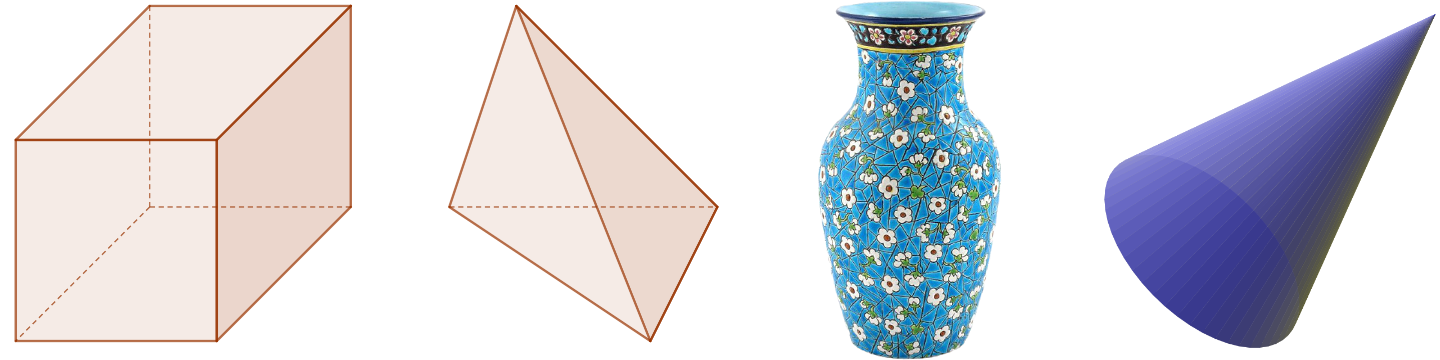
\includegraphics[width=0.8\textwidth]{tu/多面体1.png}
    % \caption*{\texttt{各种立体图形}}
\end{figure}

多面体的表面,同属一个平面的部分,称为\textbf{多面体的面}。相邻两面公共的部分是线段,称为\textbf{多面体的棱}。
两条或多条棱相交于多面体表面一点,也是多个面的公共点,称为\textbf{多面体的顶点}。上图的六面体中,有$ABCD$、
$ABB'A'$、$BCC'B'$、$CDD'C'$、$DAA'D'$、$A'B'C'D'$六个面,$AB$、$B'C'$、$DD'$等十二条棱,
$A,B,C,D$等八个顶点。多面体不同顶点之间的连线,如果不在多面体任何一面中,就称为\textbf{多面体的对角线}。
上图的六面体中,$AC'$和$B'D$是对角线,$AB'$和$B'D'$不是对角线。

多面体的面总是多边形。多面体每一面所在平面都把空间分为两半。
如果多面体总在其中一侧,就说它是\textbf{凸多面体}。凸多面体的面总是凸多边形。
以下我们只讨论凸多面体,凡提到多面体,都是指凸多面体。

围成多面体的平面数目,一般用来为多面体命名。比如六个平面围成的多面体,叫做六面体;
十个平面围成的多面体,叫做十面体。
平面与多面体相交,得到它的子集,称为平面截多面体得到的\textbf{截面}。

\section{四面体和棱锥}
多面体的面总是多边形。多边形的边就是多面体的棱,也就是它所在平面与其他面相交的部分。
因此多面体每个面至少和另三个面相交,才能形成多边形。最简单的多面体是\textbf{四面体}。
它的每个面和另三个面相交,形成三角形。四面体的面就是四个三角形。每两个三角形的公共边,就是四面体的棱。
四面体有六条棱,每三条棱交于一点。四面体有四个顶点。

四面体是最基本的多面体。任何多面体总能看作若干个四面体拼接而成。

每个面都是正三角形的四面体,称为\textbf{正四面体}。不同的正四面体大小不同,形状一致。正四面体所有的棱长度相等。
设正四面体棱长为$a$,则每个面的面积为$\frac{\sqrt{3}}{4}a^2$。

过正四面体$ABCD$一个顶点$D$向另三点确定的平面作垂线,
记垂足为$O$,则$O$为$\triangle ABC$的中心。$|AO|=|BO|=|CO|=\frac{\sqrt{3}}{3}a$。
$\angle DOA$是直角,所以根据勾股定理,$|DO| = \frac{\sqrt{6}}{3}a$。
我们称$DO$为正四面体中$D$出发的\textbf{高线}。

\begin{figure}[h] 
    % \vspace{-4pt}
    \centering
    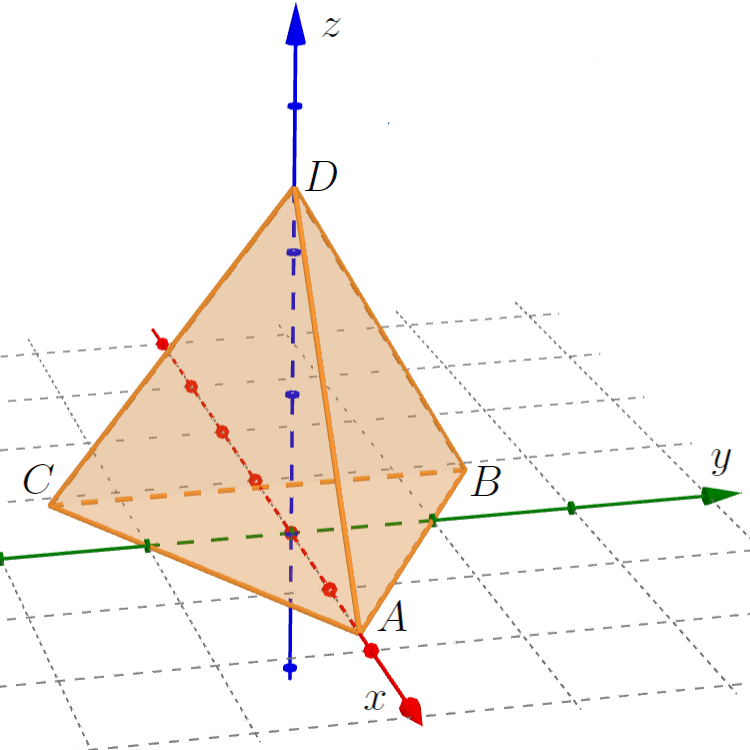
\includegraphics[width=0.6\textwidth]{tu/正四面体2.png}
    % \caption*{\texttt{各种立体图形}}
\end{figure}

\begin{et}
    求正四面体相邻两面所成的角。
\end{et}
\begin{so}
    设正四面体$ABCD$边长为$a$。过顶点$D$作平面$ABC$的垂线,记垂足为$O$。
    
    以$O$为原点,以$OA$为$x$轴作直角坐标系,使得$B,C$点坐标分别在第二、第三象限。
    $|OA|=\frac{\sqrt{3}}{3}a$,所以$A,B,C$坐标分别为$(-\frac{\sqrt{3}}{3}a, 0, 0)$、$(-\frac{\sqrt{3}}{6}a, \frac{1}{2}a, 0)$、
    $(-\frac{\sqrt{3}}{6}a, -\frac{1}{2}a, 0)$,$D$点坐标为$(0,0,\frac{\sqrt{6}}{3}a)$。
    于是平面$ABC$的方程为
    $$z=0.$$
    $AB$和$y$轴的交点为$(0,\frac{1}{3}a,0)$,所以平面$ABD$的方程为
    $$\sqrt{3}x + 3y + \frac{\sqrt{6}}{2}z = a.$$
    平面$ABC$的法向量是$\mathbf{n}_1 = (0,0,1)$,平面$ABD$的法向量是
    $$\mathbf{n}_2 = \frac{(\sqrt{3}, 3, \frac{\sqrt{6}}{2})}{\|(\sqrt{3}, 3, \frac{\sqrt{6}}{2})\|} = (\frac{\sqrt{2}}{3}, \frac{\sqrt{6}}{3}, \frac{1}{3}).$$
    因此两平面的夹角$\theta$满足:
    $$ \cos{\theta} = \mathbf{n}_1\cdot \mathbf{n}_2 = (0,0,1)\cdot(\frac{\sqrt{2}}{3}, \frac{\sqrt{6}}{3}, \frac{1}{3}) = \frac{1}{3}.$$
    解得$\theta = \arccos{\frac{1}{3}} \approx 70.53^\circ$。

    由于正四面体各面地位相等,因此任何两面所成的角都是$\theta$。
\end{so}

从四面体出发,可以得到一类称为棱锥的多面体。给定一平面及其中一个多边形,
从平面外一点上到多边形各个顶点连线,得到的多面体称为\textbf{棱锥}。
直观上看,棱锥是平面外一点发出的三条或以上不共面的射线被平面所截得到的。
平面外的点称为\textbf{棱锥的锥顶},
多边形称为\textbf{棱锥的底面},
其余的面是多边形相邻顶点和锥顶构成的三角形,称为\textbf{棱锥的侧面}。锥顶到底面的距离称为\textbf{棱锥的高}。
棱锥的侧面是以锥顶为公共顶点的三角形。

如果底面是$n$边形($n$为大于等于$3$的整数),就称棱锥为$n$棱锥。四面体就可以称为三棱锥。

棱锥的棱可以分为两类。一类是底面的边,称为\textbf{棱锥的底棱};一类是底面顶点和锥顶的连线,称为\textbf{棱锥的侧棱}。
每条侧棱是相邻两侧面的公共边。相邻的侧棱是同一个侧面的边,不相邻的侧棱所在的平面截棱锥的截面,称为\textbf{棱锥的对角面}。
对角面就是底面的对角线和锥顶构成的三角形。

\begin{figure}[h] 
    % \vspace{-4pt}
    \centering
    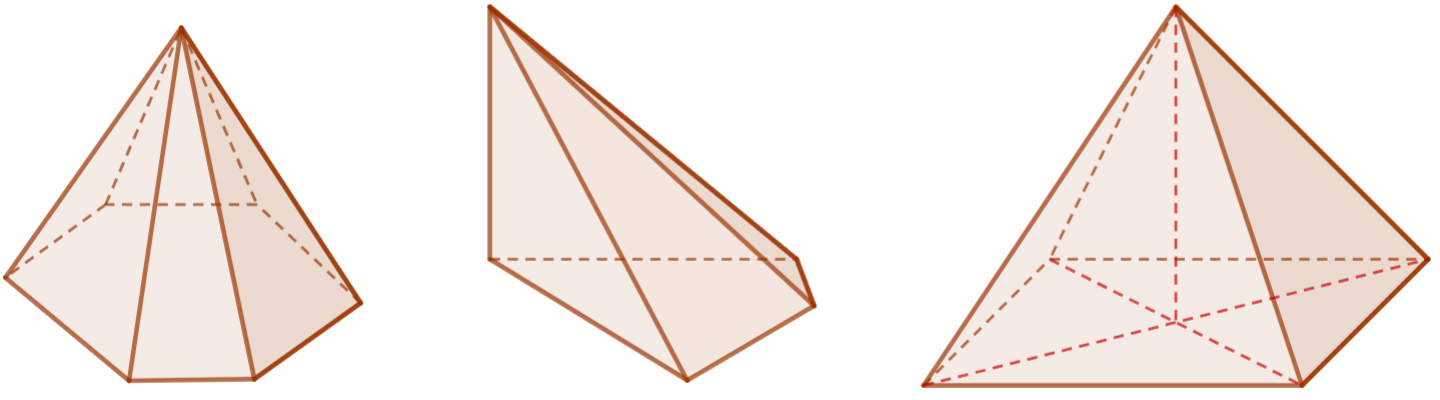
\includegraphics[width=0.8\textwidth]{tu/棱锥1.png}
    % \caption*{\texttt{各种立体图形}}
\end{figure}

棱锥底面的多边形可以用对角线剖分成多个三角形。每个三角形作为底面,棱锥锥顶作为锥顶的三棱锥,合起来就是原棱锥。
这说明任何棱锥都是四面体拼合而成。

如果棱锥底面是正多边形,且锥顶在底面的投影是正多边形的中心,就说棱锥是\textbf{正棱锥}。正四面体就是一种正三棱锥。
正棱锥的各个侧面都是全等的等腰三角形,都和底面成相等的角。这些等腰三角形的高都相等,称为正棱锥的\textbf{斜高}。
正棱锥的侧棱长度都相等,且和底面成相等的角。
\begin{xt}
    \mbox{}\\
    \indent 1. 正八面体是由两个正四棱锥底面重合拼成的多面体。每个面都是全等的正三角形,每个顶点都是四个面的交点。求正八面体相邻两面的夹角。\\
    \indent 2. 是否有四个面都是直角三角形的四面体?如果有,请举出例子;如果没有,请证明。\\
    \indent 3. 四面体$ABCD$中,过顶点$A$的三个面都是直角三角形。$A$到平面$BCD$的垂足为$H$。$H$和三角形$BCD$有何关系?试证明之。
\end{xt}

\section{平行六面体和棱柱}

\begin{wrapfigure}[6]{r}{0.42\textwidth} %this figure will be at the right
    \vspace{-40pt}
    \flushright
    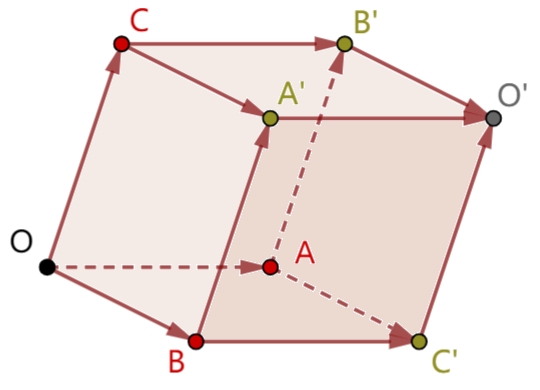
\includegraphics[width=0.4\textwidth]{tu/平行六面体1.png}
\end{wrapfigure}

如果说四面体是立体空间中的三角形,那么平行六面体就是立体空间中的平行四边形。

平行六面体可以由三个不共轴向量$\vv{OA},\vv{OB},\vv{OC}$出发,通过不断构建平行四边形得到。
首先,三个向量中每两个向量可以构建一个平行四边形。比如$\vv{OA},\vv{OB}$可以确定平行四边形$AOBC'$,
其中向量$\vv{OC'}=\vv{OA}+\vv{OB}$。同理可以得到$\vv{OA'}=\vv{OB}+\vv{OC}$、$\vv{OB'}=\vv{OC}+\vv{OA}$。

接下来,向量$\vv{OA'},\vv{OB'},\vv{OC}$又可以确定平行四边形$A'CB'O'$,
其中$\vv{OO'}=\vv{OA}+\vv{OB}+\vv{OC}$。此外可以验证,
向量$\vv{OA'},\vv{OB},\vv{OC'}$以及向量$\vv{OA},\vv{OB'},\vv{OC'}$分别确定的平行四边形的第四个顶点也是$O'$。

$O,A,B,C,A',B',C',O'$这八个顶点确定的六面体就叫作\textbf{平行六面体},记为平行六面体$O-ABC-A'B'C'-O'$或$AOBC'-B'CA'O'$,
简记为平行六面体$OABC$。

平行六面体的八个顶点可以看作三个不共轴向量按照“加或不加”的规则得到的所有组合:
$$ \big\{uA+vB+wC \, | \, u,v,w\in\{0,1\}\big\}.$$
有时候,我们也用$(u,v,w)$来指代各个顶点,称为顶点的\textbf{内坐标}。
比如,点$A$的内坐标是$(1,0,0)$,而点$B'$的内坐标是$(1,0,1)$。

直观上看,平行六面体的$12$条棱可以分为三组,每组四条棱都相互平行且等长,对应同一个向量。
比如$\vv{OA} = \vv{BC'} = \vv{CB'} = \vv{AO'}$ 。平行六面体的三组对面分别相互平行,
而且是全等的平行四边形;根据面的平行关系以及平行四边形的全等关系,可以推出每组各面对应的对角线平行且等长。
这些对角线称为平行六面体的\textbf{面对角线}。每个面两条对角线的交点称为平行六面体的\textbf{面心}。

平行六面体的顶点可以分为四对,每对顶点的内坐标相加恰好是$(1,1,1)$。比如$A(1,0,0)$和$A'(0,1,1)$就是一对。
每对顶点的连线称为平行六面体的\textbf{体对角线}。四条体对角线交于一点:$X=\frac{1}{2}O'$,
它平分这四条对角线。我们称$X$为平行六边形的\textbf{体心}或\textbf{中心}。

和平行四边形类似,我们也可以定义一些特殊的平行六面体。如果向量$A,B,C$相互垂直,
就说平行六面体$OABC$是\textbf{长方体}。如果向量$A,B,C$长度相等,就说平行六面体$OABC$是\textbf{菱体}。
如果向量$A,B,C$相互垂直且长度相等,就说平行六面体$OABC$是\textbf{正方体}。
可以看到,这些特殊平行六面体要求三组对面同时具有某种性质。
长方体的面都是长方形,菱体的面都是菱形,正方体的面都是正方形。

三组面的性质也可以不全相同。比如,如果$A$与$B,C$垂直,就说平行六面体$OABC$是\textbf{直斜方体};
如果只知道$A,B$垂直,就说平行六面体$OABC$是\textbf{双斜方体}。
类似定义的特殊平行六面体种类较多,此处不一一介绍。

%平行六面体的体积

\begin{wrapfigure}{r}{0.25\textwidth} %this figure will be at the right
    \vspace{-40pt}
    \flushright
    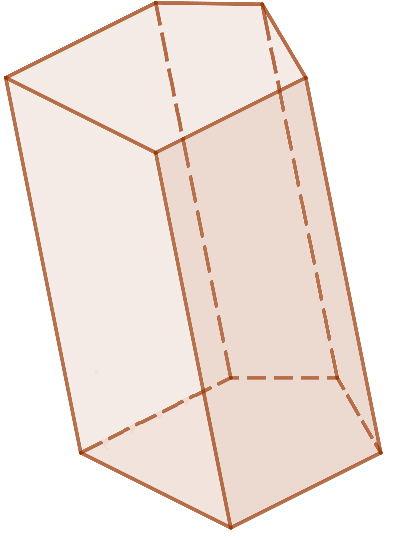
\includegraphics[width=0.24\textwidth]{tu/棱柱1.png}
\end{wrapfigure}

从平行六面体出发,可以得到一类称为棱柱的多面体。给定一平面及其中一个多边形。
将多边形所有顶点按同一个向量平移,得到一个新的多边形。新多边形所在平面和原平面平行。
连接新旧多边形对应顶点的线段,全部平行且相等。相邻的两对新旧顶点,构成一个平行四边形。
新旧多边形和这些平行四边形所在的平面围成的多面体,称为\textbf{棱柱}。

直观上看,棱柱是三条或以上不共面的直线被两个平行平面所截得到的,
对应的两个面称为\textbf{棱柱的底面}(按需要可以称为上底面和下底面),其余的面称为\textbf{棱柱的侧面}。
两底面的距离称为\textbf{棱柱的高}。
如果底面是$n$边形,就称棱柱为$\mathbf{n}$\textbf{棱柱}。比如平行六边形就是四棱柱。

棱柱的棱分为两类,一类是两个全等多边形的边,称为\textbf{棱柱的底棱},侧面连接多边形对应顶点的边,
称为\textbf{棱柱的侧棱}。每条侧棱是相邻两侧面的公共边。相邻的侧棱是同一侧面的边,
不相邻的侧棱截棱柱得到的平面,叫作\textbf{棱柱的对角面}。对角面也是平行四边形。它的一对边是不相邻的侧棱,
另一对边是两多边形对应的对角线。

棱柱底面的多边形可以用对角线剖分为多个三角形,从这个意义上来说,底面是三角形的三棱柱可以说是基本的棱柱。
平行六面体总可以看成两个三棱柱拼合而成。 

如果棱柱的底面是正多边形,且两个正多边形的中心连线与它们所在平面垂直,这样的棱柱称为\textbf{正棱柱}。
正方体就是正四棱柱。一组对面为正方形的长方体也是正四棱柱。如果棱柱的侧面总与底面垂直,这样的棱柱称为\textbf{直棱柱}。
正棱柱总是直棱柱。

如果棱柱两相邻侧面都与底面垂直,那么根据定理\ref{tm:1-3-100},它们的交线与底面垂直,也就是说,直棱柱的侧棱总与底面垂直。
\begin{xt}
    \mbox{}\\
    \indent 1. 证明:平行六面体的体心平分对面面心的连线。\\
    \indent 2. 证明:长方体各个对角面的面积相等。\\
    \indent 3. 试将三棱柱分为三个四面体。
\end{xt}

\section{棱台}
如前所述,
棱锥可以看成平面截发自同一点的三条或更多(不共面的)射线得到的多面体。
棱柱可以看成两平行平面截三条或更多(不共面的)平行直线得到的多面体。而棱台是介于两者之间的一种多面体。

\begin{wrapfigure}[7]{r}{0.25\textwidth} %this figure will be at the right
    \vspace{-20pt}
    \flushright
    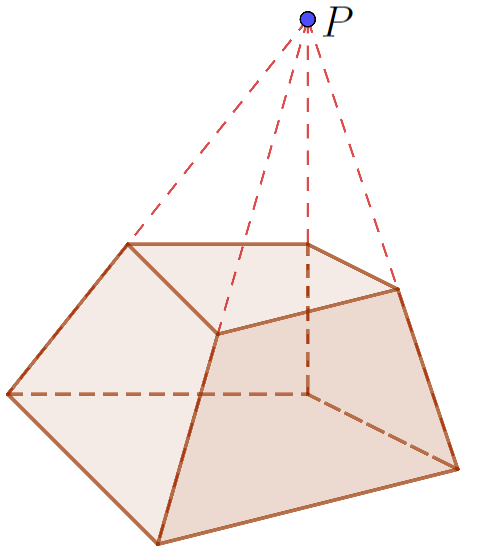
\includegraphics[width=0.24\textwidth]{tu/棱台1.png}
\end{wrapfigure}

给定一个棱锥,用平行于底面的平面,可以将它截成两部分。一部分是和原棱锥形状相同、大小不同的棱锥,
另一部分由两个形状一致、大小不一的多边形和连接它们对应顶点的线段构成的多面体,称为\textbf{棱台}。
和平面形状类比,棱台类似于梯形。

和棱柱类似,两个平行多边形称为\textbf{棱台的底面}(按需要可以称为上底面和下底面),两底面的距离称为\textbf{棱台的高}。
其余的面称为\textbf{棱台的侧面}。每个侧面都是梯形,梯形的上下底分别是上下底面的边。
如果底面是$n$边形,就称棱台为$\mathbf{n}$\textbf{棱台}。

棱台的棱分为两类,一类是两个全等多边形的边,称为\textbf{棱台的底棱},侧面连接多边形对应顶点的边,
称为\textbf{棱台的侧棱}。每条侧棱是相邻两侧面的公共边。相邻的侧棱是同一侧面的边,
不相邻的侧棱截棱柱得到的平面,叫作\textbf{棱台的对角面}。对角面也是梯形。它的一对边是不相邻的侧棱,
另一对边是两多边形对应的对角线。

棱台是平面截棱锥所得,所以,上底是下底的位似形,锥顶是位似中心。换句话说,设下底为多边形$A_1A_2\cdots A_n$,
上底是$B_1B_2\cdots B_n$,棱锥锥顶为$P$,那么存在系数$t>0$,使得:
$$\forall i\in[1,\cdots ,n],\,\,\,\vv{PB_i} = t\vv{PA_i}.$$
正棱锥截得的棱台叫作\textbf{正棱台}。正棱锥的侧棱长度相等,所以正棱台的侧棱长度也相等。

\section{正多面体}
我们知道平面形中有正多边形。正多边形是所有边长相等、所有内角相等的多边形。空间中也可以定义正多面体。

\begin{df}
    所有面都是全等的正多边形,且每个顶点都由相同个数的棱与面交汇而成的多面体,称为\textbf{正多面体}。
\end{df}

这样定义的正多面体符合我们的直观理解。要注意的是,它的定义比平面中的正多边形更严格。
正多边形有无穷多种,任给大于等于$3$的整数$n$,都可以画出正$n$边形。但空间中的正多面体只有有限多个。

考虑正多面体的某个顶点。它是若干条棱、若干个面的交点。根据定义,每面的两条棱的夹角都一样大。
假设它是$k$个面的交点,那么$k \geqslant 3$。

这个夹角是每个面的正多边形的内角。设正多边形有$m$个边,那么$m \geqslant 3$。
它的内角为$\frac{(m - 2)\cdot 180^\circ}{m}$。
$k$个内角的和小于周角。也就是说,
$$ \frac{(m - 2)\cdot 180^\circ}{m} < \frac{360^\circ}{k}.$$
解这个方程,得到$m < \frac{2k}{k - 2}$。于是
$$ \frac{2k}{k - 2} > 3.$$
解得$k < 6$。于是$k$的值只可能是$3$、$4$或$5$。

$k = 5$时,解得$m < \frac{10}{3}$,所以$m$的值只可能为$3$。

$k = 4$时,解得$m < 4$,所以$m$的值只可能为$3$。

$k = 3$时,解得$m < 6$,所以$m$的值可能为$3$、$4$或$5$。

以上一共有五种可能。也就是说,空间中一共只可能有五种正多面体。它们分别是以下形状:

% 正多面体
\begin{figure}[h]
    \vspace{4pt}
    \centering
    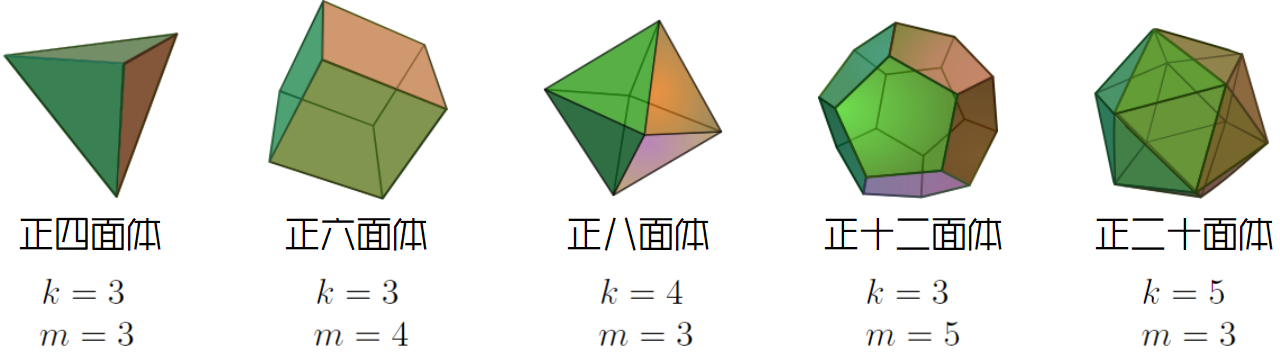
\includegraphics[width=0.8\textwidth]{tu/正多面体1.png}
    \captionsetup{justification=centering}
\end{figure}

\begin{sk}
    \mbox{}\\
    \indent 1. 如果把正多面体的定义放宽,不限定每个顶点都由相同个数的棱与面交汇而成,是否有别的正多面体?试举例说明。\\
    \indent 2. 如果把正多面体的定义放宽,只要求每个面都是全等的多边形,是否有别的正多面体?试举例说明。
\end{sk}

\begin{xt}
    \mbox{}\\
    \indent 1. 设有底面是正方形的正四棱锥,侧棱与底边等长。把两个这样的正四棱锥底面重合,使两者的顶点关于底面所在平面对称。证明:这样得到的多面体是正八面体。\\
    \indent 2. 如上得到的正八面体,记重合的底面的四个顶点为$A$、$B$、$C$、$D$,记关于正方形$ABCD$对称的两顶点为$P$、$Q$。\\
    \indent 2.1. 证明:$\triangle PAC$是等腰直角三角形。\\
    \indent 2.2. 设正八面体棱长为$a$,证明:它的表面积为$2\sqrt{3}a^2$。\\
    \indent 2.3. 证明:正八面体的体积为$\frac{\sqrt{2}}{3}a^3$。\\
    \indent 3. 正十二面体有几个顶点?正二十面体有几个顶点?\\
    \indent 4. 把正十二面体相邻的面的中心连起来,证明:得到的多面体是正二十面体。\\
    \indent 5. 把正二十面体相邻的面的中心连起来,证明:得到的多面体是正十二面体。
\end{xt}


\chapter{旋转体}

多面体是一类简单的立体形状。另一种容易想到的立体形状是\textbf{旋转体}。
空间中,把给定平面上的图形绕平面上的某条直线旋转,围成的形状就叫旋转体。该直线称为旋转体的\textbf{旋转轴}。
旋转体对应着平面形中的圆形。

\section{圆锥、圆柱和圆台}

给定平面中的直角三角形$OAB$,将它绕着直角边$OA$所在直线旋转一周,就得到一个\textbf{圆锥},
记为圆锥$OAB$。$O$称为\textbf{圆锥的锥顶},旋转轴$OA$称为\textbf{圆锥的轴},它的长度叫做\textbf{圆锥的高}。
斜边$OB$称为\textbf{圆锥的母线},
旋转得到的面称为\textbf{圆锥的侧面},另一直角边$AB$旋转得到的面称为\textbf{圆锥的底面}。

给定平面中的矩形$OO'AB$,将它绕着边$OO'$所在直线旋转一周,就得到一个\textbf{圆柱},
记为圆柱$OO'AB$。旋转轴$OO'$称为\textbf{圆柱的轴},它的长度叫做\textbf{圆柱的高}。$AB$称为\textbf{圆柱的母线},
它旋转得到的面称为\textbf{圆柱的侧面},
另两边$O'A$、$OB$旋转得到的面称为\textbf{圆柱的底面}。

给定平面中的直角梯形$OO'AB$,将它绕着直角腰$OO'$所在直线旋转一周,就得到一个\textbf{圆台},记为圆台$OO'AB$。
旋转轴$OO'$称为\textbf{圆台的轴},它的长度叫做\textbf{圆台的高}。$AB$称为\textbf{圆台的母线},旋转得到的面称为\textbf{圆柱的侧面},
另两边$OA$、$O'B$旋转得到的面称为\textbf{圆台的底面}。

另一种定义是将平面中一直线$m$绕另一直线$h$旋转。如果两直线平行,那么得到的形状称为\textbf{全圆柱面};
如果两直线相交,那么得到的形状称为\textbf{全圆锥面}。
$h$称为旋转轴,而$m$称为母线,相交直线的交点就是锥顶。用两平行平面截全圆柱面,如果平面垂直于旋转轴,就得到圆柱;
如果不垂直,得到的形状称为\textbf{斜圆柱}。用平面截全圆锥面,如果平面垂直于旋转轴,从锥顶到平面的部分就是圆锥;
如果不垂直,从锥顶到平面的部分称为\textbf{斜圆锥}。用两平行平面截全圆锥面,如果平面垂直于旋转轴,就得到圆台;
如果不垂直,得到的形状称为\textbf{斜圆台}。

显然,圆锥和圆柱分别和正棱锥、正棱柱、正棱台相似,但没有侧棱。圆台和圆锥的关系,与棱台和棱锥的关系相似。

一般来说,一点绕一直线旋转,得到的总是一个圆。圆心就是圆所在的平面和直线的交点。用向量的语言来说,
设旋转轴$h$的方向向量是$\mathbf{h} = (0,0,1)$,向量$\vv{OA}$的长度为$a>1$,则$A$绕$h$旋转,
得到的是满足$\|\vv{OP}\| = a$且$\vv{OP}\cdot\mathbf{h}=\vv{OA}\cdot\mathbf{n}$的点$P$的集合。
设点$A,P$的坐标分别为$(a_x,a_y,a_z)$,$(p_x,p_y,p_z)$,则$P$是方程组:
$$
\left\{
\begin{array}{rl}
    p_x^2+p_y^2+p_z^2 &= a_x^2+a_y^2+a_z^2 \\
    p_z &= a_z
\end{array}
\right.
$$
即
$$
\left\{
\begin{array}{rl}
    p_x^2+p_y^2 &= a_x^2+a_y^2 \\
    p_z &= a_z
\end{array}
\right.
$$

的解集。这是一个圆,它所在平面是$z=a_z$,圆心为$(0,0,a_z)$,半径为$\sqrt{a_x^2+a_y^2}$。

将这个结论运用到圆锥、圆柱和圆台上,可以知道:圆锥$OAB$的底面是一个圆,圆心就是底面和轴的交点,
半径就是$|OA|$,称为\textbf{圆锥的半径}。
圆柱$OO'AB$的底面是两个大小一样的圆,圆心就是底面和轴的交点,半径就是$|OA|$,称为\textbf{圆柱的半径}。
圆台的底面是两个圆,圆心分别是对应平面和轴的交点,半径分别是$|O'A|$和$|OB|$,
分别称为\textbf{圆台的上底半径}和\textbf{下底半径}。

更进一步,我们可以得到圆锥、圆柱和圆台的方程。全圆锥面中,设$A$在母线$m$上。
设$m$的方向向量为$(\cos{\theta}, 0, \sin{\theta})$,$m$中一点$A$的坐标为$(t\cos{\theta}, 0, t\sin{\theta})$,
则它对应的点$P$满足
$$
\left\{
\begin{array}{rll}
    p_x^2+p_y^2 &= a_x^2+a_y^2 &= t^2\cos^2{\theta} \\
    p_z &= a_z &= t\sin{\theta}
\end{array}
\right.
$$
因此,全圆锥面是以下方程的解集:
$$ x^2 + y^2 = \frac{z^2}{\tan^2{\theta}}$$
其中$\theta$是轴和母线的夹角。而圆锥可以看做全圆锥面的锥顶$( 0,0,0)$和平面$z=z_0$之间的部分,也可以写作:
$$ x^2 + y^2 \leqslant \frac{z^2}{\tan^2{\theta}} , \quad 0\leqslant z \leqslant z_0.$$
圆台可以看做全圆锥面在平行平面$z=z_0>0$和$z=z_1 > z_0$之间的部分,也可以写作:
$$ x^2 + y^2 \leqslant \frac{z^2}{\tan^2{\theta}} , \quad z_0\leqslant z \leqslant z_1.$$
类似地,设全圆柱面的母线为$m = \mathbb{R}(0,0,1)+(a,0,0)$,$m$中一点$A$的坐标为$(a, 0, t)$,则它对应的点$P$满足
$$
\left\{
\begin{array}{rl}
    p_x^2+p_y^2 &= a^2 \\
    p_z &= a_z = t
\end{array}
\right.
$$
因此,全圆柱面是以下方程的解集:

$$ x^2 + y^2 = a^2$$

其中$a$是轴和母线的距离,也是底面的半径。而圆柱可以看做全圆柱面在平行平面$z=0$和$z=z_0$之间的部分,也可以写作:

$$ x^2 + y^2 \leqslant a^2 , \quad 0\leqslant z \leqslant z_0.$$

%\section{圆锥、圆柱、圆台的侧面}

\section{球}

圆锥、圆柱和圆台分别是直角三角形、矩形和直角梯形按轴旋转得到的,如果把圆心过旋转轴的圆按轴旋转,
得到的就是\textbf{球}。球是日常生活中常见的形状。你能说说,日常生活中哪些物品的形状可以用球来概括?

设圆的半径为$a$,圆心为$O$,圆绕着过$O$的旋转轴$h$旋转一周,得到球$\circledast(O,a)$。
$O$称为球的\textbf{球心},$a$称为\textbf{球的半径}。

球还有另一种定义:空间中到一点距离不超过定值$a$的点的集合,就是球$\circledast(O,a)$。这两种定义是等价的,
我们可以通过分别求出相应的方程来证明。

首先看用旋转定义的球。设圆$(O,a)$上的点为$A(a\cos{\theta}, 0, a\sin{\theta})$,
则它绕$\mathbf{h} = (0,0,1)$引出的直线一周得到的点$P$满足
$$
\left\{
\begin{array}{rl}
p_x^2+p_y^2 &= a^2\sin^2{\theta} \\
p_z &= a_z = a\cos{\theta}
\end{array}
\right.
$$
即
$$ p_x^2 + p_y^2 + p_z^2 = a^2.$$
也就是说,球是以下方程的解集:
$$ x^2 + y^2 + z^2 \leqslant a^2.$$
另一方面,空间中的点$P$到原点(圆$(O,a)$的圆心)的距离不超过$a$,就是说$\|\vv{OP}\| \leqslant a$​,
因此这样定义的球,也是方程
$$ x^2 + y^2 + z^2 \leqslant a^2$$
的解集。这说明两种定义是等价的。

球的表面称为球面。球面的方程是:
$$ x^2 + y^2 + z^2 = a^2.$$
换句话说,球面是到一点距离为定值的点的集合。球面任一点到球心的线段及其长度称为\textbf{球的半径}。
过球面任一点和球心的直线与球交于另一点。连接两点的线段及其长度称为\textbf{球的直径}。

圆关于圆心对称,也关于过圆心的任何直线对称。球的对称性与之类似。球关于球心对称,也关于过球心的任何直线、
任何平面对称。

用平面截球,得到的截面是什么形状呢?

考虑平面$z=z_0$,代入球的方程,得到
$$ x^2 + y^2 \leqslant a^2-z_0^2 $$
$|z_0|<a$时,方程的解集是一个圆(圆盘),称为\textbf{平面与球相交},交集称为\textbf{截面圆}。截面圆的圆心为$(0,0,z_0)$,
半径是$\sqrt{a^2-z_0^2}$。$z_0=0$时,圆心为球心,半径为$a$,我们把过球心的平面对球的截面称为\textbf{球的大圆};
$z_0\neq 0$时,半径小于$a$,$|z_0|$越小,半径越大。

$z_0=\pm a$时,方程分别只有$(a,0,0)$和$(-a,0,0)$一个解,
平面和球恰交于一点,称为\textbf{平面与球相切},该面称为\textbf{球的切面},交点称为\textbf{切点}。
切面中过切点的直线与球也只有一个交点,
称为\textbf{球的切线}。

$|z_0|>a$时,平面与球无交点,称为\textbf{相离}。

球的切面垂直于球心和切点的连线,因此切线也垂直于球心和切点的连线。反之,设$A$是球$O$面上一点,
经过$A$且垂直于$OA$的直线和平面就是球的切线和切面。

我们知道,地球大致可以看成一个球。很多与地球有关的研究中,我们假设地球是一个球,球心称为地心。
为了方便讨论,我们假设地球自转轴经过地心。与地球球面相交于两点,分别是南北两极点。
过两极的平面截地球得到的大圆,称为经线。垂直于自转轴的平面截地球得到的圆,称为纬线。
其中过地心的平面截得的大圆称为赤道。这样,用经线和纬线的交点,可以定位球面上的点。一般的球面上,
我们也可以沿用这些术语。

\chapter{空间形的体积}

生产和实践中,常常会遇到容量和占位相关的问题。比如,仓库、运输机、航母的升降间是否能容纳特定型号的粮食、战车或飞机?
修补一条堤坝需要多少土方?热水瓶能容纳多少水?这些问题背后,涉及到空间形状的大小问题。
体积的概念,就是用来衡量空间形状的大小。

和长度、面积一样,体积可以有两种理解。从相对的意义上来说,空间形状的体积是它的大小相对某个单位体积形状的大小的比值。
从绝对的意义上来说,体积就是空间形状内部点的“多少”。点、线、面按照定义是没有体积的。从没有体积的概念出发,
得到体积的概念,需要复杂的定义过程,我们不做介绍。这里我们只讨论相对意义上的体积。

和面积一样,体积是一个数。规定了立体空间的长度、长度单位和面积单位,我们规定立体空间的体积单位是棱长为$1$的正方体。
棱长为$1$的正方体,体积为$1$,称为\textbf{单位正方体}或\textbf{方元}。关于体积,也有以下两条公理:
\begin{po}{\textbf{全等公理}}\label{po:4}
    全等的形状体积相等。
\end{po}
\begin{po}{\textbf{加法公理}}\label{po:5}
    把一个形状分为若干部分,各个部分的体积之和等于整体的体积。
\end{po}
从这两条公理出发,我们来研究简单多面体的体积。

\section{平行六面体的体积}

正方体是平行六面体的特殊情形。既然我们用正方体定义单位体积,以此出发,我们来研究平行六面体的体积。

从正方体出发,自然要讨论长方体的体积。

设长方体的长、宽、高分别是正整数$a,b,c$,根据加法公理,它的体积是$abc$个方元体积之和,因此根据全等公理,
它的体积是$abc$。反之,设长方体的长、宽、高分别是$\frac{1}{a},\frac{1}{b},\frac{1}{c}$,其中$a,b,c$是正整数,
则$abc$个它的体积之和是$1$,于是它的体积是$\frac{1}{abc}$。
于是,如果长方体的长、宽、高分别是有理数$\frac{n_a}{m_a},\frac{n_b}{m_b},\frac{n_c}{m_c}$,
则体积为$n_an_bn_c$个体积为$\frac{1}{m_am_bm_c}$的长方体体积之和,即为$\frac{n_an_bn_c}{m_am_bm_c}$。
一般来说,长方体的长、宽、高分别是正数$a,b,c$,则体积为:
$$ V = abc.$$
这就是长方体的体积公式。从公式可以得到:如果一个长方体的长、宽、高分别是另一个长方体长、宽、高的$t_a,t_b,t_c$倍,
那么它的体积是后者的$t_at_bt_c$倍。如果两个长方体底面积相等,那么体积之比等于高之比。
如果两个长方体高相等,那么体积之比等于底面积之比。如果一个正方体的棱长是另一个正方体棱长的$t$倍,
那么它的体积是后者的$t^3$倍。

从向量的角度来看,以基向量$\mathbf{e}_x, \mathbf{e}_y, \mathbf{e}_z$为棱构建的单位正方体,体积为$1$。
以$a\mathbf{e}_x, b\mathbf{e}_y, c\mathbf{e}_z$为棱构建的长方形,体积为$abc$。

对一般的平行六面体,我们希望找出它的体积与方元体积之比。设平行六面体由向量$\mathbf{a},\mathbf{b},\mathbf{c}$构建,
我们尝试用以下映射表示它的体积,记为$V(\mathbf{a},\mathbf{b},\mathbf{c})$。
这是一个三元映射,我们希望它满足以下的性质:
\begin{enumerate}
    \item $V(\mathbf{e}_x, \mathbf{e}_y, \mathbf{e}_z) = 1.$ 
    \item $\forall s,t$,$V(s\mathbf{a}_1+t\mathbf{a}_2,\mathbf{b},\mathbf{c}) = sV(\mathbf{a}_1,\mathbf{b},\mathbf{c})+tV(\mathbf{a}_2,\mathbf{b},\mathbf{c})$,$V(\mathbf{a},s\mathbf{b}_1+t\mathbf{b}_2,\mathbf{c}) = sV(\mathbf{a},\mathbf{b}_1,\mathbf{c})+tV(\mathbf{a},\mathbf{b}_2,\mathbf{c})$,$V(\mathbf{a},\mathbf{b},s\mathbf{c}_1+t\mathbf{c}_2) = sV(\mathbf{a},\mathbf{b},\mathbf{c}_1)+tV(\mathbf{a},\mathbf{b},\mathbf{c}_2)$。
    \item $V(\mathbf{a},\mathbf{a},\mathbf{c}) = 0$,$V(\mathbf{a},\mathbf{b},\mathbf{a})=0$,$V(\mathbf{a},\mathbf{b},\mathbf{b})=0$。
\end{enumerate}
前两个性质对应两条公理和方元体积为$1$的设定。第三个性质说明点、线、面体积为$0$。从第三个性质出发,可以推出:
\begin{tm}{\textbf{体积的反称性}}\label{tm:3-0-0}
    给定向量$\mathbf{a},\mathbf{b},\mathbf{c}$,则它们相关的平行六面体体积满足以下性质:
    \begin{align}
        V(\mathbf{a},\mathbf{b},\mathbf{c}) &= -V(\mathbf{a},\mathbf{c},\mathbf{b}). \notag \\
        V(\mathbf{a},\mathbf{b},\mathbf{c}) &= -V(\mathbf{b},\mathbf{a},\mathbf{c}). \notag \\
        V(\mathbf{a},\mathbf{b},\mathbf{c}) &= -V(\mathbf{c},\mathbf{b},\mathbf{a}). \notag 
    \end{align}
\end{tm}
换言之,将映射$V$的任何两个自变量交换位置,值变为原来的相反数。这说明这样定义的体积可正可负。
我们把这样的体积称为\textbf{有向体积},把有向体积的绝对值称为\textbf{绝对体积},或简称体积。

方元的绝对体积总是$1$,而有向体积则可以是$\pm 1$。我们来逐个查看:
$V(\mathbf{e}_x, \mathbf{e}_y, \mathbf{e}_z) = 1$ ,因此
$$ V(\mathbf{e}_x, \mathbf{e}_z, \mathbf{e}_y) = V(\mathbf{e}_y, \mathbf{e}_x, \mathbf{e}_z)  = V(\mathbf{e}_z, \mathbf{e}_y, \mathbf{e}_x)  = -1.$$
于是
$$ V(\mathbf{e}_z, \mathbf{e}_x, \mathbf{e}_y) = V(\mathbf{e}_y, \mathbf{e}_z, \mathbf{e}_x)   = 1.$$
我们把方元分成了两类,一类的有向体积为$1$,另一类为$-1$。
%可以看出,有向体积为$1$,对应向量遵循右手法则;有向体积为$-1$,对应向量遵循左手法则。

一般来说,设$\mathbf{a} = a_x\mathbf{e}_x + a_y\mathbf{e}_y + a_z\mathbf{e}_z$、
$\mathbf{b} = b_x\mathbf{e}_x + b_y\mathbf{e}_y + b_z\mathbf{e}_z$、
$\mathbf{c} = c_x\mathbf{e}_x + c_y\mathbf{e}_y + c_z\mathbf{e}_z$,则根据第二个性质,
可以把$V(\mathbf{a},\mathbf{b},\mathbf{c})$展开成$27$项,
每一项都是$\mathbf{a},\mathbf{b},\mathbf{c}$各自坐标分量乘以$V(\mathbf{e}_i, \mathbf{e}_j, \mathbf{e}_k)$的形式,
其中$\mathbf{e}_i, \mathbf{e}_j, \mathbf{e}_k$是相同或不同的基向量。根据第三个性质,
如果其中两个向量相同,那么$V(\mathbf{e}_i, \mathbf{e}_j, \mathbf{e}_k)=0$。
因此只需要考虑$\mathbf{e}_i, \mathbf{e}_j, \mathbf{e}_k$两两不同的情况,即上面逐个查看的$6$项:
\begin{align}
    V(\mathbf{a},\mathbf{b},\mathbf{c}) = & a_xb_yc_zV(\mathbf{e}_x, \mathbf{e}_y, \mathbf{e}_z) + a_yb_zc_xV(\mathbf{e}_y, \mathbf{e}_z, \mathbf{e}_x) + a_zb_xc_yV(\mathbf{e}_z, \mathbf{e}_x, \mathbf{e}_y) \notag\\ 
    &+ a_xb_zc_yV(\mathbf{e}_x, \mathbf{e}_z, \mathbf{e}_y) + a_yb_xc_zV(\mathbf{e}_y, \mathbf{e}_x, \mathbf{e}_z) + a_zb_yc_xV(\mathbf{e}_z, \mathbf{e}_y, \mathbf{e}_x) \notag\\
    = & a_xb_yc_z + a_yb_zc_x + a_zb_xc_y - a_xb_zc_y - a_yb_xc_z - a_zb_yc_x. \notag
\end{align}

这就是平行六面体的有向体积。平行六面体的体积就是有向体积的绝对值。
\begin{et}
    求向量$(1,-0.5,0)$、$(0,1,0.5)$,$(0,0.5,1)$构建的平行六面体的体积。
\end{et}
\begin{so}
    根据平行六面体的体积公式,它的有向体积为
    $$ 1\cdot 1\cdot 1 + (-0.5)\cdot 0.5\cdot 0 + 0\cdot 0\cdot 0.5 - 1\cdot 0.5\cdot 0.5 - (-0.5)\cdot 0\cdot 1 - 0\cdot 1\cdot 0 = 0.75.$$
    体积为$0.75$。
\end{so}

\begin{sk}
    \mbox{} \\
    \indent 1. 空间基向量的有向体积和它们的顺序有什么关系?  \\
    \indent 2. 空间向量的体积和平面向量的面积有什么类似的地方?
\end{sk}

\section{等积原理}

从平行六面体的体积出发,能否得到其它多面体和立体形状的体积呢?这里介绍一个有力的结论:\textbf{等积原理}。
它结合了相对和绝对意义上的体积的概念,深刻揭示了不同形状的体积之间的关系。
本阶段我们不证明等积原理,把它作为公理引入。
\begin{po}{\textbf{等积原理}}\label{po:6}
    给定空间中两个形状$X,Y$和两个平行平面$\gamma_1,\gamma_2$,如果位于$\gamma_1,\gamma_2$之间且平行于$\gamma_1,\gamma_2$的任何平面$\gamma$截$X,Y$得到的截面面积都相等,那么$X,Y$在$\gamma_1,\gamma_2$之间的部分体积相等。
\end{po}

例如:左侧多面体$X$和右侧多面体$Y$分别被平行于平面$\gamma_1,\gamma_2$的平面所截,
前者的截面是五边形,后者的截面是三角形。
如果不论被$\gamma_1,\gamma_2$之间的哪个平行于$\gamma_1,\gamma_2$的平面所截,
截出来的五边形和三角形面积总相等,那么根据等积原理,$X$和$Y$在$\gamma_1,\gamma_2$之间的部分的体积相等。

据唐代李淳风记载,等积原理是南朝梁数学家祖暅发现的。祖暅利用等积原理,解决了球体积计算的问题。
因此,后世也把这个定理称为\textbf{祖暅原理}。等积原理可以看做平面中“同底等高面积相同”结论的“升级版”。
比如,根据等积原理,斜棱柱的体积等于同底等高直棱柱的体积。
\begin{et}
    证明长方体的对角面把它分成体积相等的两部分。
\end{et}
\begin{so}
    设有长方体$ABCD-A'B'C'D'$,它夹在平行平面$ABCD$和平面$A'B'C'D'$之间。考虑对角面$BB'D'D$,
    它把长方体分为两部分。用平行于平面$ABCD$的平面$\gamma$截这两部分,
    得到两个全等三角形(分别全等于$\triangle ABD$和$\triangle BCD$),
    因此截面面积相等。根据等积原理,这两部分在平面$ABCD$和平面$A'B'C'D'$之间的部分体积相等,即它们体积相等。
\end{so}
\begin{sk}
    \mbox{}\\
    平面中,给定两平行直线$l_1,l_2$和两个封闭图形$X,Y$。
    如果$l_1,l_2$之间任何平行于$l_1$的直线与$X,Y$的交集是等长的线段,$X,Y$夹在$l_1,l_2$间的部分的面积是否相等?
\end{sk}
\begin{xt}
    \mbox{}\\
    \indent 1. 证明:斜棱柱的体积等于同底等高直棱柱的体积。\\
    \indent 2. 给定空间中两个形状$X,Y$和两个平行平面$\gamma_1,\gamma_2$,
    如果位于$\gamma_1,\gamma_2$之间且平行于$\gamma_1,\gamma_2$的任何平面$\gamma$截$X,Y$得到的截面面积都成同一比例,比值为$c\in\mathbb{Q}$,
    证明:$X,Y$在$\gamma_1,\gamma_2$之间的部分体积之比是$c$。
\end{xt}

\section{棱柱、棱锥和棱台的体积}

首先来看棱柱的体积。

设棱柱上下底面所在平面分别是$\gamma_1,\gamma_2$。在$\gamma_1$上作面积和棱柱底面积相等的长方形$ABCD$,
过长方形四边分别作垂直于$\gamma_1$的平面。这四个平面和$\gamma_1,\gamma_2$围成一个长方体。
$\gamma_1,\gamma_2$之间任意平行于它们的平面截棱柱和长方体,截面分别是和底面全等的多边形,因此面积相等。
根据等积原理,棱柱的体积和这个长方体相等。长方体的体积等于长乘宽乘高,即底面积乘以高。
它的高是平面$\gamma_1,\gamma_2$之间的距离。我们定义棱柱的高为上下底面之间的距离,则可以得到棱柱的体积公式:
\begin{tm}\label{tm:3-2-0}
    棱柱的体积等于底面积乘以高。
\end{tm}
根据棱柱的体积公式,我们知道:\textbf{底面积相等,高相等的棱柱,体积相等}。
这个性质和平行四边形的性质类似。

接下来看棱锥的体积。过锥顶$P$作平行于底面所在平面$\gamma_1$的平面$\gamma_2$,
我们考虑$\gamma_1,\gamma_2$之间平行于$\gamma_1$的平面$\gamma$截棱锥的截面。
截面是底面的相似多边形。设$\gamma_1,\gamma_2$距离为$h$,$\gamma,\gamma_2$的距离为$g$,
则截面和底面的相似比是$\frac{g}{h}$,面积比是$\frac{g^2}{h^2}$。如果两个棱锥底面积相等,
并且锥顶到底面距离(称为棱锥的高)相等,把这两个棱锥底面放置在同一个平面上,
用锥顶和底面之间平行于底面的平面截这两个棱锥,那么各自截面的面积和相应的底面积之比相等。因此,根据等积原理:
\begin{tm}\label{tm:3-2-10}
    底面积相等,高相等的棱锥,体积相等。
\end{tm}
这个定理和三角形的性质类似。我们知道三角形是同底等高的平行四边形面积的一半,
据此,我们来研究棱锥体积和同底等高棱柱体积的关系。

从最简单的情形出发:我们假设棱锥和棱柱的底面是同一个三角形,棱锥的锥顶是棱柱的一个顶点。
这时,棱锥就是四面体。设棱柱为$ABC-A'B'C'$,棱锥为$A'ABC$。

如下图,平面$A'BC$和$A'B'C$将三棱柱分为三个四面体:$A'ABC$、$A'B'BC$和$A'B'C'C$。
其中,四面体$A'B'C'C$可以看作底面为$A'B'C'$,锥顶为$C$的三棱锥。它的底面积和棱锥$A'ABC$底面积相同,高相等,
所以根据定理\ref{tm:3-2-10},它的体积和四面体$A'ABC$的体积相等。

% 三棱柱体积
\begin{figure}[h]
    \vspace{4pt}
    \centering
    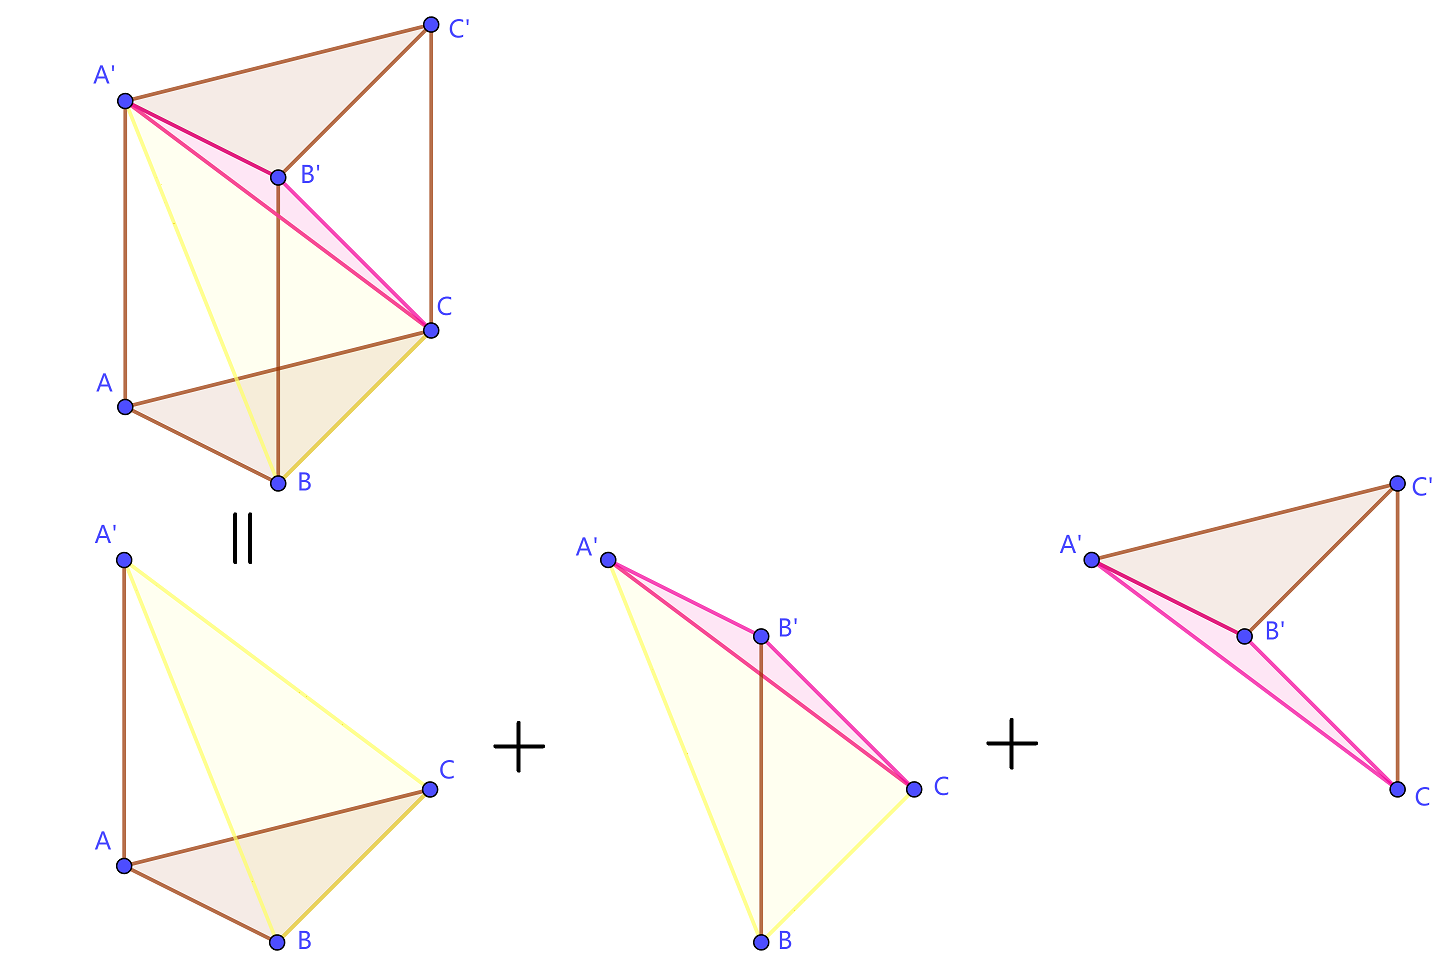
\includegraphics[width=0.8\textwidth]{tu/三棱柱体积1.png}
    \captionsetup{justification=centering}
\end{figure}

另一方面,四面体$A'B'BC$和$A'B'C'C$都可以看作底面在平面$B'C'CB$上,锥顶为$A'$的三棱锥。
它们的底面:$\triangle B'BC \simeq \triangle B'C'C$,所以根据定理\ref{tm:3-2-10},体积相等。
这说明,三棱柱由三个体积相等的四面体组成,因此它的体积是四面体$A'ABC$的三倍。

根据等积定理,三棱锥和三棱柱如果底面积相等,高相等,则棱锥的体积是棱柱体积的三分之一。

对于一般的棱柱和棱锥,我们可以将它们的底面剖分为三角形,因此,
它们的体积分别等于相应的三棱柱和三棱锥体积之和。因此,对于一般的棱柱和棱锥,也有:
\begin{tm}\label{tm:3-2-20}
    如果棱柱和棱锥的底面积相等,高相等,则棱锥的体积是棱柱体积的三分之一。
\end{tm}
因此,从棱柱的体积公式可以立刻得到棱锥的体积公式:
\begin{tm}\label{tm:3-2-30}
    棱柱的体积等于底面积乘以高除以三。
\end{tm}

最后来看棱台的体积。棱台可以看做棱锥被平行于底面的平面截去带锥顶的部分得到,
因此,它的体积等于补全后的大棱锥体积减去小棱锥体积。已知棱台上下底面积为$S_{\text{上}},S_{\text{下}}$,高为$h$,
则可以先求出大小棱锥的体积,作差得到棱台体积。

设补全后的大小棱锥高为$h_{\text{大}},h_{\text{小}}$,则$h_{\text{大}} = h_{\text{小}} + h$。棱台上下底面积之比为
$$ \frac{S_{\text{上}}}{S_{\text{下}}} = \frac{h_{\text{小}}^2}{h_{\text{大}}^2} $$
联立两个方程,解得
$$ 
    \left\{\,\,
    \begin{array}{cl}
        h_{\text{小}} &= \frac{h\sqrt{S_{\text{上}}}}{\sqrt{S_{\text{下}}} - \sqrt{S_{\text{上}}}} \\
        h_{\text{大}} &= \frac{h\sqrt{S_{\text{下}}}}{\sqrt{S_{\text{下}}} - \sqrt{S_{\text{上}}}} \\
    \end{array}
    \right.
$$
因此棱台体积为:
\begin{align}
    \text{棱台的体积} &= \text{大棱锥的体积} - \text{小棱锥的体积} \notag \\
    &= \frac{1}{3}S_{\text{下}}h_{\text{大}} - \frac{1}{3}S_{\text{上}}h_{\text{小}}\notag \\
    &= \frac{h}{3}\left(S_{\text{上}} + S_{\text{下}} + \sqrt{S_{\text{上}}S_{\text{下}}}\right)\notag 
\end{align}
\begin{tm}\label{tm:3-2-40}
    上下底面积为$S_{\text{上}},S_{\text{下}}$,高为$h$的棱台,体积为$\frac{h}{3}\left(S_{\text{上}} + S_{\text{下}} + \sqrt{S_{\text{上}}S_{\text{下}}}\right)$。
\end{tm}
可以看到,如果上底缩为一点,则上底面积为$0$,这时棱台变为棱锥;如果上底和下底全等,这时棱台变为棱柱。
% \begin{sk}
%     \mbox{}\\
%     \indent 1. ?\\
%     \indent 2. ?
% \end{sk}

\begin{xt}
    \mbox{}\\
    \indent 1. 底面是长为$4$、宽为$3$的长方形,高为$2$的四棱柱、四棱锥,体积分别是多少?\\
    \indent 2. 棱长为$3$的正四面体,体积是多少?\\
    \indent 3. 平面$\gamma$上有一梯形$ABCD$。$l$是平面外一条平行于梯形上底$AD$的直线。
    $l$到$\gamma$的距离为$3$,梯形上底长度为$2.6$、下底长度为$3.5$,梯形的高为$1.9$。
    $l$上有距离为$2.6$的两点$P,Q$。连接$PA$、$PB$、$QC$、$QD$,这样的多面体称为\textbf{畚}。
    求多面体$PQ-ABCD$的体积。
\end{xt}

\section{圆柱、圆锥和圆台的体积}
使用等积原理,不难从棱柱、棱锥和棱台的体积,推出圆柱、圆锥和圆台的体积。

半径为$r$,高为$h$的圆柱的方程可以写为
$$ x^2 + y^2 \leqslant r^2 , \quad 0\leqslant z \leqslant h.$$
任何与底面平行的平面$z=z_0$截圆柱,得到的是半径为$r$的圆。
因此,在圆柱底面所在平面作面积等于$\pi r^2$的长方形,过长方形各边作垂直底面的平面,和两底面围成长方体。
根据等积原理,这个长方体的体积等于圆柱的体积。于是可以得到圆柱体积公式:
\begin{tm}\label{tm:3-3-0}
    半径为$r$,高为$h$的圆柱,体积为$\pi r^2h$。
\end{tm}

锥顶为原点、半径为$r$、高为$h$的圆锥的方程可以写为
$$ x^2 + y^2 \leqslant \frac{r^2z^2}{h^2} , \quad 0\leqslant z \leqslant h.$$
任何与底面平行的平面$z=z_0$截圆锥,得到的是半径为$\frac{r^2z_0^2}{h^2}$的圆,面积为$\frac{\pi r^2z_0^2}{h^2}$。
因此,在圆锥底面所在平面$z=h$作面积等于$\pi r^2$的长方形,以圆点为锥顶,作它到长方形各顶点的连线,是为一四棱锥。
平面$z=z_0$截该四棱锥,得到一个长方形,面积为$\frac{\pi r^2z_0^2}{h^2}$,和截圆锥得到的圆面积相等。
因此,根据等积原理,这个四棱锥的体积等于圆锥的体积。于是可以得到圆锥体积公式:
\begin{tm}\label{tm:3-3-10}
    半径为$r$,高为$h$的圆锥,体积为$\frac{1}{3}\pi r^2h$。
\end{tm}

上底半径为$r_{\text{上}}$、下底半径为$r_{\text{下}}$,高为$h$的圆台,可以看作补全后的大圆锥减去小圆锥后的部分。
经过类似棱台的计算可以得到,大小圆锥的高分别为:
$$
\left\{
\begin{array}[]{cl}
    h_{\text{大}} &= \frac{hr_{\text{下}}}{r_{\text{下}} - r_{\text{上}}} \\
    h_{\text{小}} &= \frac{hr_{\text{上}}}{r_{\text{下}} - r_{\text{上}}} \\
\end{array}
\right.
$$
于是圆台体积为:
\begin{align}
    \text{圆台的体积} &= \text{大圆锥的体积} - \text{小圆锥的体积} \notag \\
    &= \frac{1}{3}\pi r_{\text{下}}^2h_{\text{大}} - \frac{1}{3}\pi r_{\text{上}}^2h_{\text{小}}\notag \\
    &= \frac{1}{3}\pi\left(r_{\text{上}}^2 + r_{\text{下}}^2 + r_{\text{上}}r_{\text{下}}\right)h\notag 
\end{align}
即:
\begin{tm}\label{tm:3-3-20}
    上下底半径分别为$r_{\text{上}}$、$r_{\text{下}}$,高为$h$的圆台,体积为
    $$\frac{1}{3}\pi \left(r_{\text{上}}^2 + r_{\text{下}}^2 + r_{\text{上}}r_{\text{下}}\right)h.$$
\end{tm}

不难看出,如果把圆柱、圆锥的底面积记为$S$,把圆台上下底面积记为$S_{\text{上}},S_{\text{下}}$,
则圆柱、圆锥和圆台的体积公式和棱柱、棱锥和棱台的体积公式完全一致。
\begin{sk}
    \mbox{}\\
    \indent 1. 方程$x^2 + (y - z)^2 = \frac{r^2z^2}{h^2}$,$0\leqslant z\leqslant h$
    确定的空间形状和圆锥$x^2 + y^2 = \frac{r^2z^2}{h^2}$,$0\leqslant z\leqslant h$一样吗?它们的体积一样吗?\\
    \indent 2. 考虑全圆锥面$x^2 + y^2 = z^2$和全圆柱面$x^2 + (z - 4)^2 = 9$围成的空间形状。它的体积是多少?
\end{sk}

\begin{xt}
    \mbox{}\\
    \indent 1. 半径为$5$、高为$2$的圆柱、圆锥,体积分别是多少?\\
    \indent 2. 上底半径为$3$、下底半径为$7$、高为$5$的圆台,体积是多少?\\
    \indent 3. 考虑点$(0,0,0)$、$0,0,4$、$(3,0,1)$确定的三角形。
    将它分别绕$x$轴、$y$轴、$z$轴旋转,得到的空间形状的体积各是多少?
\end{xt}

\section{球的体积}
球的体积较难直接看出。我们可以从平面截球的截面面积入手。

圆心为原点、半径为$r$的球的方程可以写为:
$$ x^2 + y^2 + z^2 = r^2.$$
用离圆心$z_0$的平面$z = z_0$截球,得到半径为$\sqrt{r^2 - z_0^2}$的圆盘,
面积为$\pi(r^2 - z_0^2)$。

考虑下底在$Oxy$平面、上底在$z=r$平面,半径为$r$、高为$r$的圆柱:
$$ x^2 + y^2 = r^2, \quad 0\leqslant z \leqslant r $$
平面$z = z_0$截该圆柱得到的截面面积为$\pi r^2$。

考虑锥顶在原点、上底在$z=r$平面、半径为$r$、高为$r$的圆锥,
$$ x^2 + y^2 = z^2, \quad 0\leqslant z \leqslant r $$
平面$z = z_0$截该圆锥得到的截面面积为$\pi z_0^2$。

因此,考虑圆柱中挖去圆锥得到的形状,根据等积原理,它的体积等于半个球($z>0$部分)的体积。
于是,
\begin{align}
    \text{球的体积} &= 2\cdot\left(\text{圆柱的体积} - \text{圆锥的体积}\right) \notag \\
    &= 2\left(\pi r^2\cdot r - \frac{1}{3}\pi r^2\cdot r \right)\notag \\
    &= \frac{4}{3}\pi r^3\notag 
\end{align}
即:
\begin{tm}\label{tm:3-3-30}
    半径为$r$的球,体积为$\frac{4}{3}\pi r^3$。
\end{tm}

\begin{sk}
    \mbox{}\\
    \indent 1. 半径为$r$的球面,面积是多少?\\
    \indent 2. 球面能否展开成为平面形状?如果不能,如何求它与单位面积的比值?
\end{sk}

\begin{xt}
    \mbox{}\\
    \indent 1. 从棱长为$4$的正方体中挖出一个最大的球,剩余部分的体积是多少?\\
    \indent 2. 全圆柱面$y^2+z^2=r^2$和$x^2+z^2=r^2$围成的形状称为\textbf{牟合方盖}。求牟合方盖的体积。\\
    \indent 3. 圆心为原点、半径为$r$的球在平面$z = z_0$和$z = r$之间的部分,称为球缺。求球缺的体积。 \\
    \indent 4. 平面$y = 0$上有方程为$(x - 4)^2 + z^2 = 4$的圆,将它绕$z$轴旋转一周围成的空间形状称为\textbf{镯}。\\
    \indent 4.1. 求该镯的方程。\\
    \indent 4.2. 求平面$z = z_0$截该镯的截面面积。\\ 
    \indent 4.3. 试通过与平放的圆柱对比,求该镯的体积。\\
    \indent 4.4. 试推导镯的体积公式。
\end{xt}


% %%%%%%%%%%%%%%%%%%%%%%%%%% %
%                            %
%          APPENDIX          %
%                            %
% %%%%%%%%%%%%%%%%%%%%%%%%%% %

\begin{appendix}

\chapter{空间形的表示法}

为了方便讨论空间形,我们希望在纸面上快速便捷地表示空间中的点、直线、平面等基本形状。
讨论平面形状时,我们自然地将纸面作为形状所在的平面。讨论空间中的形状时,
我们没法在纸面上完整表示立体图形,所以需要一套统一约定的折衷方法,方便交流。
我们把这样的方法称为\textbf{作图法}或\textbf{画法}。

人类自古以来就在探索作图法。距今两万年的壁画上,就有用线条表示动物和地形的创作。
人类对作图法的探索有两个方向,一个致力于在平面上真实地还原人眼看到的景物,
另一个致力于用简练记号表述空间中的对象。前者发展出以透视法为基础的艺术绘画技法,
后者发展出以地图、工程图等为代表的实用绘图技法。
下面介绍的属于后者,是数学中一种常用的简便作图法。

\section{在空间中画平面}

空间中的平面是没有边界的。为了在有限的纸面上表示平面,我们选用一定的形状框定边界,表示一个平面,
称为平面的\textbf{示形}。要注意的是,这样表示的平面其实是平面的一部分,但不妨碍我们想象它是无边际延伸开来的。

我们约定用常见的平行四边形表示平面。平行四边形的长边长度一般介于短边长度的$1.5$至$3$倍之间,
长短边的锐角夹角一般是$45$度角。

一般来说,水平位置的平面(称为\textbf{水平面}),用上下对边水平的平行四边形表示,竖直位置的平面(称为竖立面),
用左右对边竖直的平行四边形表示。矩形一般表示正对视线的竖直平面。完全侧对视线的竖直平面,用$45$度角的上下对边表示。

平面的名字一般标记在示形内部,靠近其某个顶点。

当一个平面示形的一部分被其它平面遮住时,我们用虚线表示被遮住部分的边界。如果虚线使得画面过于繁杂难辨,
可以连虚线也不画。

用平行四边形表示平面,意味着我们降低了对真实性的要求,比如舍弃了近大远小的性质。
因此作出的图形往往“不真实”。例如,一个水平面,我们看不出它到底位于我们上方还是下方。
为此我们约定,\textbf{所有水平面均处于视线下方},即我们总在俯视这些平面。
这样,水平面靠下的点离我们较近,靠上的点离我们较远。

\section{在水平面中画平面图形}

已知一个平面形的样子,如何把它画在空间中某个水平面里?

我们把平面形所在的图称为平面图,把要画的图称为立体图。首先在立体图中画出水平面。
为了方便,设示形的水平边长度为非水平边的$2$倍,夹角为$45$度。这个比例系数和夹角在下面画平面图形时将一直使用。

选择平面图中一条线段、射线或直线作为\textbf{水平线}。把它画进立体图时,画成水平方向,
长度不变。与它平行的线段、射线、直线,也画成水平方向,线段长度不变。

平面图中垂直于水平线的线段、射线或直线(称为\textbf{纵直线}),把它画进立体图时,
画成与平面非水平对边平行的方向($45$度角),线段的长度要除以$2$。

要将平面图中一点画进立体图中,可以先在平面图中作它到水平线和纵直线的垂线。
这样,该点就成了水平线和纵直线的交点,于是可以在立体图中作出对应的点。

平面图中其它位置的线段、射线或直线,在其中取两点(线段一般取端点,射线取端点和较远一点,
直线取较远两点)。将两点按上述方法画进立体图中,再连出对应的线段、射线或直线。

约定平面图中的上下左右关系在立体图中不变。但立体图中的上下关系应理解为前后关系,
即靠上的在后(较远),靠下的在前(较近)。

\section{在一般平面中画平面图形}

在一般平面中画平面图形是复杂的操作。从原则上来说,违背了简便作图法的精神,
容易产生既不简便、真实性也低的困境。因此,如果可以选择在水平面中画平面图形,最好不要在非水平面中画。

和在水平位置的平面中画平面图形的方法类似,我们需要在立体图中示形的对边中选择一个\textbf{主边}和一个\textbf{副边}。
水平面中,我们选择水平方向的对边为主边,非水平方向的对边为副边。一般平面中,需要自行选择边和副边。
主边长度和副边长度之比称为\textbf{斜变系数},比如水平位置平面的斜变系数为$2$。

选定之后,主方向将对应平面图中的水平线,副方向将对应平面图中的纵直线。
平面图中平行于水平线的线段、射线、直线,按主边方向画出,线段长度不变。
平面图中垂直于水平线的线段、射线、直线,按副边方向画出,线段长度要除以斜变系数。

要将平面图中一点画进立体图中,可以先在平面图中作它到水平线和纵直线的垂线。
这样,该点就成了水平线和纵直线的交点,于是可以在立体图中作出对应的点。

平面图中其它位置的线段、射线或直线,在其中取两点(线段一般取端点,射线取端点和较远一点,
直线取较远两点)。将两点按上述方法画进立体图中,再连出对应的线段、射线或直线。

把平面图形画到非水平面中的时候,平面图中的上下左右关系在立体图中可能改变。
为此,作图时需要注意保持一致性,否则将产生错误的结果。

\section{画空间直角坐标系}

以上作图法中,其实已经用到了坐标系的想法。比如,平面图中的水平线可以看作坐标轴横轴,
纵直线可以看作坐标轴纵轴。我们把平面图中一点画到立体图中时,过它作到水平线和纵直线的垂线,实际上就在确定它的坐标。

我们可以直接在立体图中画出直角坐标系。一般来说,选定的基底$\mathbf{e}_x,\mathbf{e}_y,\mathbf{e}_z$,
表示三个两两垂直的单位向量,对应三条射线。在立体图中,直角坐标系有多种画法。

选定一点为原点,过原点往右作水平射线,这条射线可以是$x$轴或$y$轴正半部分。如果设它为$x$轴正半,
那么过原点往右上$45$度角作射线,是为$y$轴正半;如果设它为$y$轴正半,那么过原点往左下$45$度角作射线,
是为$x$轴正半。最后过原点往上作竖直射线,是为$z$轴正半。这种画法称为\textbf{右手正斜式}。
将$x$轴和$y$轴互换,则称为\textbf{左手正斜式}。

另一种画法从$z$轴开始。过原点往上作竖直射线,是为$z$轴正半。将其顺时针旋转$120$度,得到$x$轴正半;
顺时针再旋转$120$度,得到$y$轴正半。这种画法称为\textbf{右手对称式}。将$x$轴和$y$轴互换,则称为\textbf{左手对称式}。

更一般的画法则继续向透视法靠拢。比如参考两点透视画出水平位置的矩形,以此确定$x$轴和$y$轴。
我们不在此展开,只介绍正斜式画法。

正斜式画法与前面的平行四边形表示法兼容。从左下为$x$轴的右手对称式出发,容易看出,
$Oxy$就是水平面。为了方便,我们在它的示形基础上画坐标系。选好长短边长度后,水平上边就是$y$轴,
非水平的左边就是$x$轴。将代表射线的箭头画在平行四边形对应的顶点,然后将这两边等分,标上坐标刻度。
$z$轴(竖轴)按$y$轴长度标上刻度。朝反方向延伸可以画出各坐标轴的负半部分,并标上刻度。

按照坐标轴刻度,可以找出$Oxy$中点的位置。比如,要画出坐标为$(1,2,0)$的点,可以在$x$轴找到刻度为$1$的点,
过它作平行于$y$轴的直线(水平线);在$y$轴找到刻度为$2$的点,过它作平行于$x$轴的直线;
两线交点就是坐标为$(1,2,0)$的点。

对于不在$Oxy$中的点,可以先画出它在$Oxy$上的投影点。比如,要画出坐标为$(1,2,3)$的点,
可以先画出$(1,2,0)$,然后过它作平行于$z$轴的直线。由于往上为$z$轴正向,所以对于正数$3$,
往上数三个单位长度,即为$(1,2,3)$。如果要画坐标为$(1,2,-3)$的点,则向下数三个单位长度。
为了清楚表明点在空间中的位置,可以保留投影点,并将投影点与$x$轴、$y$轴用虚线连线,将目标点和投影点用虚线连线。

\chapter{空间向量与公理}

下面验证:根据向量定义的点、直线、平面符合平面公理、平直公理、交面公理和补充的平行公理。

\section{平面公理}
首先来看平面公理。任取不共轴三点$A,B,C$,则$A-C,B-C$直无关,
因此$ \{sA+tB+(1 - s - t)C \, | \,s, t\in\mathbb{R}\}$是$A,B,C$确定的平面。

\section{平直公理}
再来看平直公理。
如果点$P,Q$在平面$ \{sA+tB+(1 - s - t)C \, | \, s,t\in\mathbb{R}\}$中,那么存在$s_1, t_1, s_2, t_2$使得
\begin{align}
P &= s_1A + t_1B + (1 - s_1 - t_1)C \notag \\
Q &= s_2A + t_2B + (1 - s_2 - t_2)C \notag 
\end{align}
直线$PQ$是集合$\{uP+(1-u)Q \, | \, u\in \mathbb{R}\}$,其中任一点$U = uP+(1-u)Q$可以用$A,B,C$表示为
\begin{align}
U &= uP+(1-u)Q \notag \\
&= (us_1 + (1-u)s_2)A + (ut_1 + (1-u)t_2)B + (u(1 - s_1 - t_1) + (1-u)(1 - s_2 - t_2))C  \notag \\
&= (us_1 + (1-u)s_2)A + (ut_1 + (1-u)t_2)B + (1 - (us_1 + (1-u)s_2) - (ut_1 + (1-u)t_2))C \notag
\end{align}
因此$U$在平面$ABC$中。这说明向量表示的空间符合平直公理。

\section{交面公理}
接下来验证交面公理。
如果两平面$\gamma_1, \gamma_2$交于点$C$,记$\gamma_1 = \mathbb{R}A_1+\mathbb{R}B_1+C$,$\gamma_2 = \mathbb{R}A_2+\mathbb{R}B_2+C$。
其中$(A_1,B_1)$直无关,$(A_2,B_2)$直无关。两平面公共点可以表示为让以下等式成立的$s_1,t_1,s_2,t_2$:
$$ s_1A_1+t_1B_1+C = s_2A_2+t_2B_2+C. $$
以上等式可以转为:
$$ s_1A_1+t_1B_1 - s_2A_2 - t_2B_2 = \mathbf{0}. $$
根据空间的根本性质,四个向量总是直相关。所以存在不全为零的四个实数$s_1,t_1,s_2,t_2$使上式成立。
由于$(A_1,B_1)$直无关,$(A_2,B_2)$直无关,所以$s_1A_1+t_1B_1$和$s_2A_2 + t_2B_2$为零向量时,
$s_1,t_1,s_2,t_2$必然全为零。然而$s_1,t_1,s_2,t_2$不全为零,所以$s_1A_1+t_1B_1$和$s_2A_2 + t_2B_2$不为零向量。
于是这时$s_1A_1+t_1B_1+C = s_2A_2+t_2B_2+C\neq C$是两平面另一个公共点。这说明向量表示的空间符合交面公理。

\section{平行公理}
我们主要验证平行线共面的性质。
平面中,两条直线平行,当且仅当它们的直部是同一条过原点的直线。我们用这个方法来判定空间中直线的平行关系。设有两直线$l_1\parallel l_2$,那么它们是同一条过原点的直线平移而成:
\begin{align}
l_1: & \,\,\, \mathbb{R}\mathbf{a} + \mathbf{b}_1 \notag \\
l_2: & \,\,\, \mathbb{R}\mathbf{a} + \mathbf{b}_2\notag
\end{align}
所以$l_1,l_2$都在平面:$\gamma = \mathbb{R}\mathbf{a} + \mathbb{R}(\mathbf{b}_1 - \mathbf{b}_2) + \mathbf{b}_2$中。
对任意$t\in\mathbb{R}$,$l_1$中的点$t\mathbf{a} + \mathbf{b}_1 = t\mathbf{a} + 1\cdot(\mathbf{b}_1 - \mathbf{b}_2) + \mathbf{b}_2 \in \gamma$;
$l_2$中的点$t\mathbf{a} + \mathbf{b}_2 = t\mathbf{a} + 0\cdot(\mathbf{b}_1 - \mathbf{b}_2) + \mathbf{b}_2 \in \gamma$。
这说明,两条平行直线总在同一平面内,即向量表示的空间符合补充后的平行公理。

\end{appendix}


% \chapter{brouillon}

% 从直观上看,把$x$看成大地,$(x,\,\,y)$看作空中的一点,
% 那么$P(x,\,\, y)$就好像它在竖直阳光下的影子。
% $P$的特点是:
% \begin{enumerate}
%     \item 本来就在“大地”($x$轴)上的向量,经过$P$映射不变。
%     \item 垂直于$x$轴的向量(形如$(0,\,\,y)$的),经过$P$映射为零向量。
%     \item 任何向量经过$P$映射后,总在$x$轴上。
% \end{enumerate}

% 一般来说,给定两个不共轴的向量$\mathbf{a}$、$\mathbf{b}$,它们形成平面的基底。
% 因此,平面中任意向量$\mathbf{u}$总能以唯一的方式写成$\mathbf{a}$、$\mathbf{b}$的直组合:
% $$ \mathbf{u} = u_a \mathbf{a} + u_b \mathbf{b}.$$
% 我们把这个写法称为向量$\mathbf{u}$在基底$\mathbf{a}$、$\mathbf{b}$上的分解。
% 或者说,实系数对$(u_a,\,\, u_b)$是$\mathbf{u}$在$\mathbf{a}$、$\mathbf{b}$构成的坐标系中的坐标。
% 于是,我们可以定义\textbf{沿}$\mathbf{b}$\textbf{到}$\mathbf{a}$\textbf{的投影映射}。:
% $$ \mathrm{Ty}_{(\mathbf{a},\mathbf{b})} : \mathbf{u} \mapsto u_a \mathbf{a}.$$

% 当$\mathbf{a}$、$\mathbf{b}$是直角坐标系的基向量$\mathbf{e}_1$、$\mathbf{e}_2$时,
% $\mathrm{Ty}_{(\mathbf{a},\mathbf{b})}$就是前面提到的$P$。

% 如图,当$\mathbf{a}=(3,\,\,1)$、$\mathbf{b}=(1,\,\,3)$时,$\mathrm{Ty}_{(\mathbf{a},\mathbf{b})}$
% 把点$(4,\,\,4)$沿经过$(4,\,\,4)$并且与$\mathbf{b}$平行的直线移动,直到和直线$\mathbb{R}\mathbf{a}$相交。
% 得到的点就是$(4,\,\,4)$沿$\mathbf{b}$到$\mathbf{a}$的投影。
% 直观上看,就好像日光斜照,把$(4,\,\,4)$投射到“大地”$\mathbb{R}\mathbf{a}$上,形成的影子。而
% 日光的方向由$\mathbf{b}$决定。


\end{document}